% General Paper Template created by Adam Green
% Last revised 1/09/18

\documentclass[12pt]{article}

%%%%%%%%%%%%%%%%%%%%%%%%%%
% Standard packages
%%%%%%%%%%%%%%%%%%%%%%%%%%
\usepackage{amsmath,amsfonts,amsthm,amssymb}
\usepackage[margin = 2cm]{geometry}
%\usepackage{siunitx}

%%%%%%%%%%%%%%%%%%%%%%%%%%
% Graphical packages
%%%%%%%%%%%%%%%%%%%%%%%%%%
\usepackage{graphicx}
\usepackage{subfig}
\usepackage{float}
\usepackage{tikz}
%\usepackage{tikz-3dplot}
%\usepackage{pgfplots}

\graphicspath{{Figures/}} % set directory for figures


%%%%%%%%%%%%%%%%%%%%%%%%%%
% Table and Array packages
%%%%%%%%%%%%%%%%%%%%%%%%%%
\usepackage{tabu}
\usepackage{booktabs}
\usepackage{xcolor}


%%%%%%%%%%%%%%%%%%%%%%%%%%
% Citation packages
%%%%%%%%%%%%%%%%%%%%%%%%%%
\usepackage{hyperref}
%\hypersetup{citebordercolor = {0 0.75 0.75}, linkbordercolor = {0 0.75 0.75} }
\hypersetup{allcolors = {0 0.75 0.75}, allbordercolors = {0 0.75 0.75}, filecolor = {0 0.75 0.75}, linkbordercolor = {0 0.75 0.75} }
\usepackage{cleveref}

%%%%%%%%%%%%%%%%%%%%%%%%%%
% Text Formatting packages
%%%%%%%%%%%%%%%%%%%%%%%%%%
\usepackage{multicol}
\usepackage{parskip} 
\usepackage{indentfirst} 
	\setlength{\parindent}{14pt}
\usepackage{fancyhdr}
%	\pagestyle{fancy}
\usepackage{enumerate}
\usepackage{wrapfig}
\usepackage{lipsum}
\usepackage{caption}
	\captionsetup{format=hang, justification = raggedright, singlelinecheck=false}
	

%%%%%%%%%%%%%%%%%%%%%%%%%%
% Custom Commands
%%%%%%%%%%%%%%%%%%%%%%%%%%
\renewcommand{\deg}{^\circ} % Degree Symbol (only in math mode)
\renewcommand{\vec}[1]{\mathbf{#1}} % boldface vectors

\newcommand{\redline}{\textcolor{red}{\rule{\textwidth}{2.5pt} } }
\newcommand{\redmark}{\textcolor{red}{\rule[1mm]{7mm}{1mm} }}

\newcommand{\red}[1]{\textbf{\textcolor{red}{#1}}} % My standard commenting style
\newcommand{\scap}[1]{\textsc{\makeLowercase{#1}}} % Makes caps small so it doesnt SHOUT
\newcommand{\Ylm}[2]{\mathrm{Y}^{#1}_{#2}} % Spherical Harmonics
\newcommand{\crefrangeconjunction}{-}


% Math commands, first and second order partials, Laplacian
\newcommand{\evaluate}{\Bigr\rvert}
\newcommand{\ppd}[1]{\frac{\partial}{\partial#1}}
\newcommand{\ppsd}[1]{\frac{\partial^2}{\partial #1^2}}
\newcommand{\ppnd}[2]{\frac{\partial #1}{\partial #2}}
\newcommand{\ppsnd}[2]{\frac{\partial^2 #1}{\partial #2^2}}
\newcommand{\lap}{\nabla^2}

% Quantum bra- ket- commands
\newcommand{\bra}[1]{\langle #1 |}
\newcommand{\ket}[1]{| #1 \rangle}
\newcommand{\bracket}[2]{\langle #1 | #2 \rangle}

% Redfine equation and figure references to include "Eqn. ()" and "Fig. _"
\newcommand{\figref}[1]{Fig.\ \ref{#1}}
\let\originaleqref=\eqref
\renewcommand{\eqref}{Eqn.\ \originaleqref}


% Custom matrix spacing
% Syntax: \begin{matrix}[scale]
\makeatletter
\renewcommand*\env@matrix[1][\arraystretch]{%
	\edef\arraystretch{#1}%
	\hskip -\arraycolsep
	\let\@ifnextchar\new@ifnextchar
	\array{*\c@MaxMatrixCols c}}
\makeatother

\newcommand{\email}[1]{\href{mailto:#1}{#1}}
\newenvironment{institutions}[1][2em]{\begin{list}{}{\setlength\leftmargin{#1}\setlength\rightmargin{#1}}\item[]}{\end{list}}


\begin{document}

	
%%%%%%%%%%%%%%%%%%%%%%%%%%%
% Title
%%%%%%%%%%%%%%%%%%%%%%%%%%%	
\begin{center}



	{\huge \bf Quantum Analogs}
	
	\vspace{0.5cm}
	
	\textbf{Adam Green}, \textbf{Guillermo Acuna}\\
	
	\texttt{\footnotesize \email{agree019@ucr.edu}},
	\texttt{\footnotesize \email{gacun002@ucr.edu}}
	
	\vspace{0.5cm}
	
	
	\begin{institutions}[2.25cm]
		\footnotesize
		{\it 
			Department of Physics \& Astronomy, 
			University of  California, Riverside, 
			{CA} 92521	    
		}    
	\end{institutions}

	\vspace{0.5cm}
	
\end{center}

%%%%%%%%%%%%%%%%%%%%%%%%%%%
% Abstract
%%%%%%%%%%%%%%%%%%%%%%%%%%%	
	\vspace{0.5cm}

\begin{abstract}
	In this experiment, we model the quantum mechanical wavefunction of the Hydrogen atom as a pressure wave inside a spherical cavity. The time evolution and spatial of these two waves, the wavefunction and pressure wave, are described by two different equations, the Schr\"odinger equation and wave equation respectively. However, under special conditions, the standing waves produced by these equations have striking similarity. For a spherical cavity, the angular dependence of the wave equation and Hydrogren atom are identical, and it is possible to generate standing waves inside the cavity which mimic the spherical harmonics of the Hydrogen atom. This allows us to determine $\ell$ values for each standing wave. However, the system contains a $(2\ell+1)$ degeneracy. This degeneracy can be resolved by breaking the spherical symmetry of the cavity by introducing spacing rings. Once the symmetry is broken, a quantization axis is introduced and we can resolve the $m=0$ and the $m=\pm1$ peaks in the cavity.
\end{abstract}

\section{Introduction}
Often times in physics, the specific mathematical equations used to represent physical systems can become system-independent under special circumstances. In other words, the same equations can be used to describe very different systems. One intriguing example is a parallel between the Shcr\"odinger equation and the wave equation. Both equations describe a sort of ``wave.'' In the Schr\"odinger equation, the ``wave'' is not a physical wave, but a probability wave. In the case of the wave equation, the wave is a physical pressure wave. Nonetheless, under special circumstances, these two equations can be modeled the same way.

In this experiment, we model the wavefunction of the Hydrogen atom with a physical pressure wave inside a hollow spherical cavity. This is possible because the conditions inside the spherical cavity mimic the conditions of a Hydrogen atom and the equations which describe the wavefunction and pressure wave have the same solution. We will begin by analyzing the solutions to both the Schr\"odinger equation and the wave equation.


\hrulefill

The Schr\"odinger equation is used to describe the time-evolution of a quantum mechanical system and is given by:
\begin{equation}
\label{schrodingerEqn1}
	i\hbar\ppnd{\psi}{t} = \left[-\frac{\hbar^2}{2m}\lap+ V(\vec{r},t)\right] \psi
\end{equation}
where $\psi$ is a complex wavefunction which has temporal and spatial dependence, $\psi = \psi{(\vec{r},t)}$, and $V(\vec{r},t)$ is a time and space dependent potential.

When the potential is time-independent, as in our case for the Coulomb potential $V = V(\vec{r})$, stationary states form in which the energy of the wavefunction remains constant and the Schr\"odinger equations reduces to:
\begin{equation}
\label{schrodingerEqn2}
	E \psi = \left[-\frac{\hbar^2}{2m}\lap + V(\vec{r})\right] \psi
\end{equation}
For our case, the potential will be the Coulomb potential $V(r) = -e^2/r$. Taking advantage of spherical symmetry of the potential and spherical laplacian, we may rewrite the Schr\"odinger equation in spherical coordinates:
\begin{equation}
\label{schroderEqnSphere}
	E \psi = -\frac{e^2}{r} + \frac{\hbar}{2m} \left[ \frac{1}{r^2} \ppd{r}r^2 \ppd{r} + \frac{1}{r^2\sin(\theta)}\ppd{\theta}\sin(\theta)\ppd{\theta} + \frac{1}{r^2\sin^2(\theta)} \ppsd{\varphi} \right] \psi 
\end{equation}
where the first term is the Coulomb potential. We may solve \eqref{schroderEqnSphere} with separation of variables, in which case the the solution admits the following form:
\begin{equation}
	\psi(r,\theta,\varphi) = \mathrm{Y}_\ell^m(\theta,\varphi) \, \mathrm{R}(r)
\end{equation}
The entire angular dependence of \eqref{schroderEqnSphere} is contained in the spherical harmonics $\mathrm{Y}_\ell^m(\theta,\varphi)$. Here, $\ell$ and $m$ are the two quantum numbers representing angular momentum and magnetic spin respectively. Similarly, the entire radial dependence of \eqref{schroderEqnSphere} is contained in $\mathrm{R}(r)$.

The spherical harmonics $\mathrm{Y}_\ell^m(\theta,\varphi)$ satisfy:
\begin{equation}
\label{sphericalHarmonic}
	-\left[ \frac{1}{\sin(\theta)}\ppd{\theta}\sin(\theta)\ppd{\theta} + \frac{1}{\sin^2(\theta)} \ppsd{\varphi} \right] \, \mathrm{Y}_\ell^m = \ell(\ell+1)\mathrm{Y}_\ell^m
\end{equation}
and admit solutions which are proportional to the Legendre polynomials $P_\ell^m(\cos(\theta))$ and a complex exponential:
\begin{equation}
	\mathrm{Y}_\ell^m(\theta,\varphi) \propto P_\ell^m(\cos(\theta))e^{im\varphi}
\end{equation}
The complex exponential however is not physical since it represents a quantum phase which is never observable.

The radial solution $\mathrm{R}(r)$ satisfies:
\begin{equation}
\label{radialSoln}
	- \frac{\hbar}{2m} \left[ \frac{1}{r} \ppsd{r}r + \frac{\ell(\ell+1)}{r^2} + \frac{e^2}{r} \right] \mathrm{R}(r) = E \, \mathrm{R}(r)
\end{equation}

\hrulefill

We will now shift our attention to the spherical acoustic resonator which contains a pressure wave $\rho$ whose time-evolution is described by the wave equation:
\begin{equation}
	\label{waveEqn1}
	\ppsnd{\rho}{t} = v^2 \, \lap\rho
\end{equation}
where $v$ is the velocity of the wave, and the quantity $\rho = \rho(\vec{r},t)$ represents the wave. To solve \eqref{waveEqn1}, we assume the following functional form for the pressure wave:
\begin{equation}
\label{waveSoln}
	\rho(\vec{r},t) = \mathrm{P}(\vec{r})\cos(\omega t)
\end{equation}
in which case, the wave equation reduces to the time-independent Helmholtz equation:
\begin{equation}
\label{helmholtzEqn}
	-\omega^2 \mathrm{P} = \lap \mathrm{P}
\end{equation}
We pause here to draw a parallel between the Schr\"odinger equation, \eqref{schrodingerEqn2}, and the time-independent Helmholtz equation, \eqref{helmholtzEqn}. Up to the addition of the the Coulomb potential in the Schr\"odinger equation, the two equations have the same differential form, and we expect similar solutions.

Proceeding in a similar fashion to the Schr\"odinger analysis, we take advantage of the spherical symmetry of the cavity and write \eqref{helmholtzEqn} in spherical coordinates:
\begin{equation}
\label{helmholtsSphere}
	\frac{\omega^2}{v^2} \mathrm{P} = \left[ -\frac{1}{r^2} \ppd{r}r^2\ppd{r} - \frac{1}{r^2\sin(\theta)}\ppd{\theta}\sin(\theta)\ppd{\theta} -\frac{1}{r^2\sin^2(\theta)} \ppsd{\varphi} \right] \mathrm{P}
\end{equation}
Again, up to the addition of the Coulomb potential, the spherical Helmholtz equation, \eqref{helmholtsSphere}, has the same form as the spherical Schr\"odinger equation,  \eqref{schroderEqnSphere}, so we expect similar behavior of the solutions.

We proceed in the same fashion and assume a separable solution to \eqref{helmholtsSphere} which takes the form:
\begin{equation}
	\mathrm{P}(r,\theta,\varphi) = \mathrm{Y}_\ell^m(\theta,\varphi) \mathrm{F}(r)
\end{equation}
where the entire angular dependence of the pressure wave is contained in the spherical harmonics $\mathrm{Y}_\ell^m$ just as the case with the Schr\"odinger equation. However, the radial component of the pressure wave obeys a slightly modified differential equation compared to the case of the Hydrogen atom:
\begin{equation}
	\left[ -\ppsd{r} - \frac{2}{r}\ppd{r} + \frac{\ell(\ell+1)}{r^2} \right] \mathrm{F} = \frac{\omega^2}{v^2}\mathrm{F}
\end{equation}
	
Since the Coulomb potential has no angular dependence, it does affect the angular solutions of  either the Schr\"odinger equation or the Helmholtz equation and the angular dependence of both solutions are identical. 

\red{Talk about energies}

\red{Talk about degeneracies}

	
\section{Experimental Procedure}

	\subsection{Experiment Setup}
	This experiment utilized the \emph{Quantum Analogs Controller} seen in \figref{QAController}. The ``Sine Wave Input'' on the controller is connected to the signal generator and provides the frequency of the signal inside the cavity. The ``Speaker Output'' is connected to the speaker on the cavity. The microphone from the cavity is connected to the ``Microphone Input'' on the device. This reads the signal from the cavity into the controller. The ``A/C Monitor'' port is connected to channel 2 on our oscilloscope. This is the output of the microphone from inside the cavity. Finally, we connect the ``Detector Output'' on the controller to a multimeter set to read DC voltage. The controller converts the AC microphone signal to its envelope and outputs it as a DC signal to ``Detector Output.'' A full view of our lab bench can be used for reference in \figref{experiment}.
	
	
	\subsection{Cavity Angles and Spherical Angles}
	The main apparatus for this experiment is the spherical cavity. The microphone and speaker configuration inside the cavity is characterized by the \emph{cavity angle} $\alpha$. When spherical symmetry is present, the conversion from the cavity angle $\alpha$ to polar angle $\theta$ is:
		\begin{equation}
		\label{alpha2theta}
		\cos(\theta) = \frac{1}{2}\cos(\alpha) - \frac{1}{2}
		\end{equation}
	In the appendix, \figref{ThetaAlpha} shows the relation between cosine of the polar angle $\theta$ and the cavity angle $\alpha$. When the spherical symmetry is broken however, the system is quantized about the $\vec{z}$ axis perpendicular to the table, and the cavity angle is equal to the azimuthal angle $\varphi$.
	
	\begin{figure}[H]
		\captionsetup{justification = centering}
		\centering
		\subfloat[Quantum Analogs Controller]{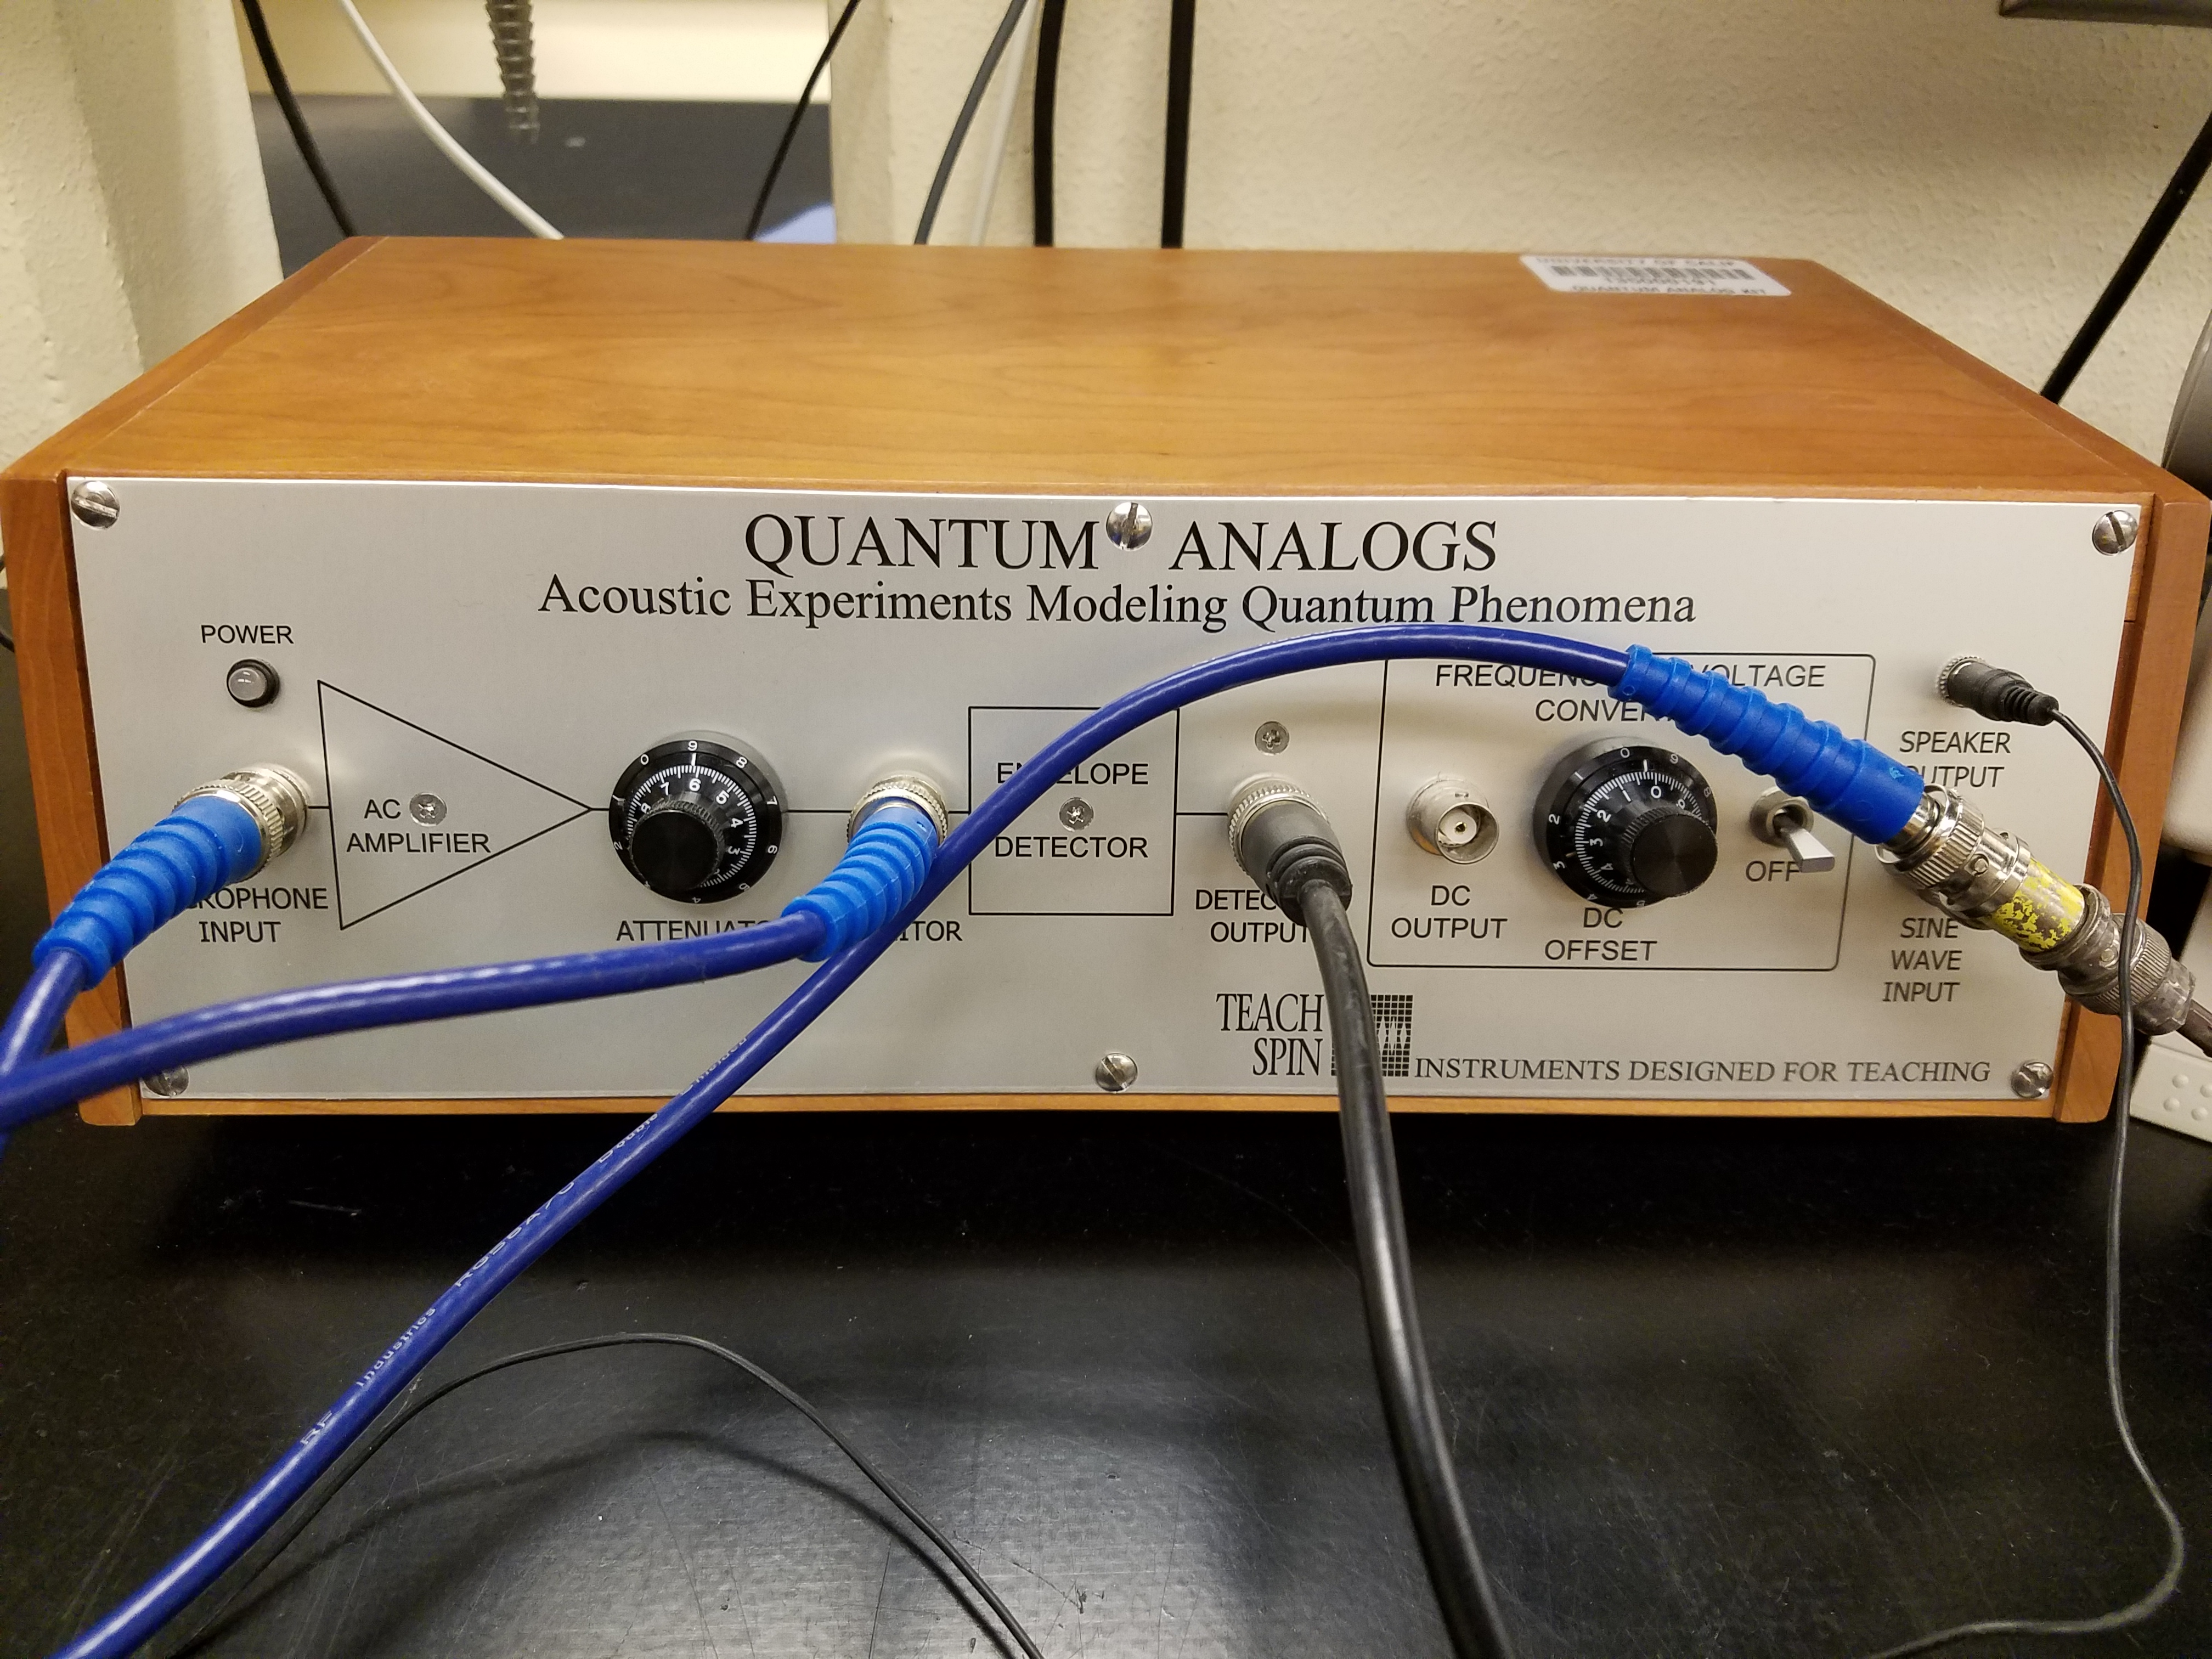
\includegraphics[width=0.4\textwidth]{Setup/AnalogsDevice}\label{QAController}}
		\qquad
		\subfloat[Lab bench]{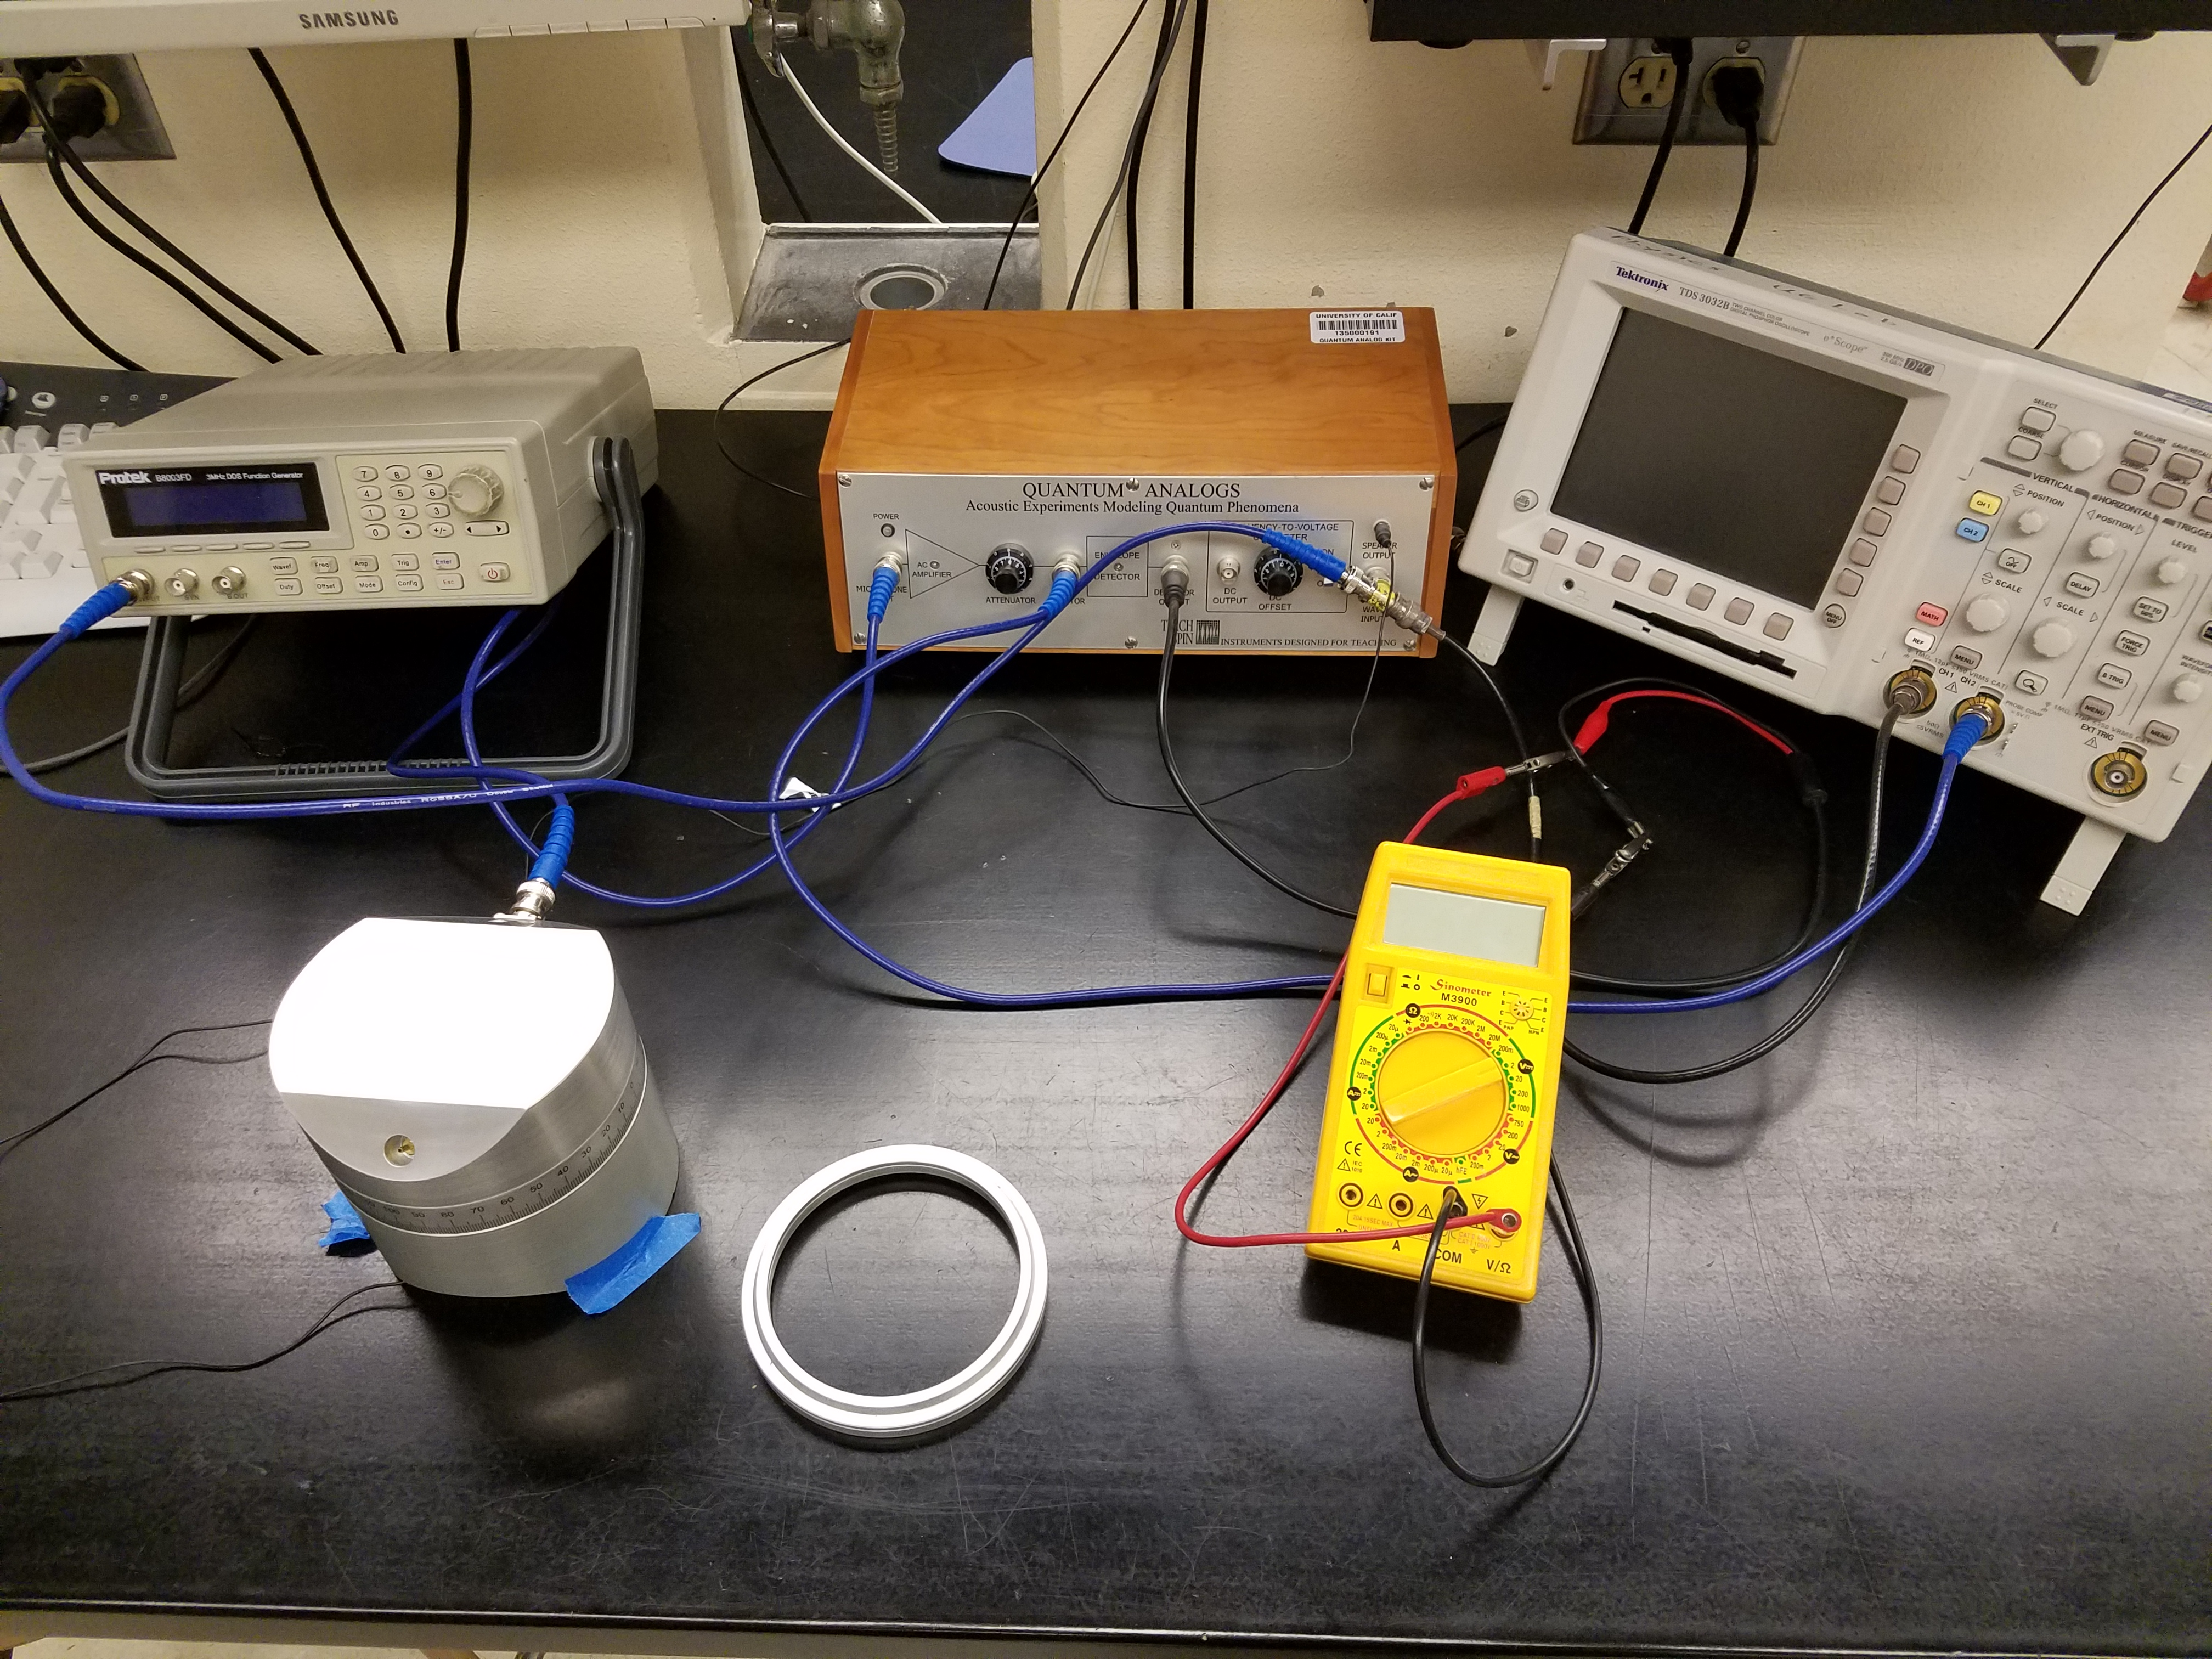
\includegraphics[width=0.4\textwidth]{Setup/Table}
		\label{Setup}}
		\caption{The \emph{Quantum Analogs Controller} \protect\subref{QAController} and our table setup up \protect\subref{Setup}}
		\label{experiment}
	\end{figure}

%		\subsection{Acoustic Resonances of the Spherical Cavity}
	
	\subsection{Frequency Spectrum}
%	Before we begin mapping out resonant frequencies, we need to find the frequency range where the cavity response is linear. We do this because the equations we seek to model are linear. To do this, we set the attenuation to maximum (10), $\alpha = 180 \deg$, and sweep the frequency from $1$ Hz to $\approx 8$ kHz in increments of $10$ Hz. The linear regime of the signal ranges from about $2$ kHz to $8$ kHz and is seen in \figref{LinRegime}. We use $10$ Hz increments simply to find the neighborhood of a resonance, as greater resolution is not required. After we found the linear regime, we lowered the attenuation to half (5.0) and obtained the spectrum of frequencies with clear resonances, see \figref{Raw50a180}. The two smaller peaks at $\approx 6.5$ kHz and $8$ kHz are products of cross talk, and thus not resonances.
	
	Since the equations we are modeling are linear differential equations, we need to determine the frequency range where the cavity response is linear. measure the frequency spectrum over the entire frequency range, with the attenuation on the Quantum Analogs device set to its maximum setting, and focus our attention to the region where the spectrum increases linearly. We determine the linear regime of frequency response is between $2$ kHz to $8.1$ kHz. The linear regime of the frequency spectrum is shown in \figref{LinRegime}. The large spikes indicate resonant frequencies. Once we determine the linear regime of the signal, we fine tune the attenuation and speaker amplitude to maximize signal and minimize cross-talk. The frequency spectrum for $\alpha = 180\deg$ and $50\%$ attenuation can be seen in \figref{Raw50a180}. The two smaller peaks at $\approx 6.5$ kHz and $8$ kHz are products of cross talk, and thus not resonances.
	
	\begin{figure}[H]
		\captionsetup{justification = justified}
		\centering
		\subfloat[Linear regime frequency spectrum with maximum attenuation]
		{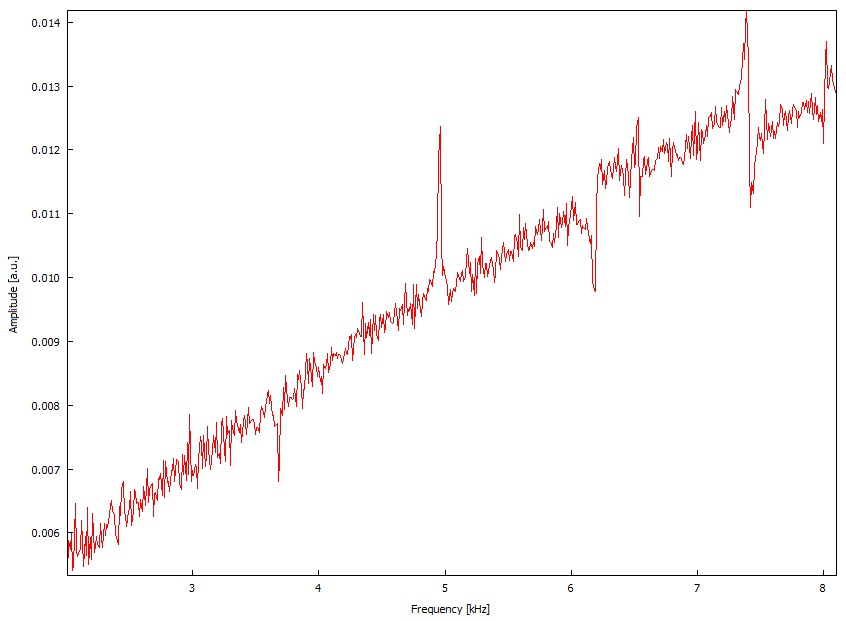
\includegraphics[width=0.4\textwidth]{2.3.2/Raw100a180.jpg}
			\label{LinRegime}}
		\qquad
		\subfloat[Linear regime frequency spectrum with half attenuated signal]{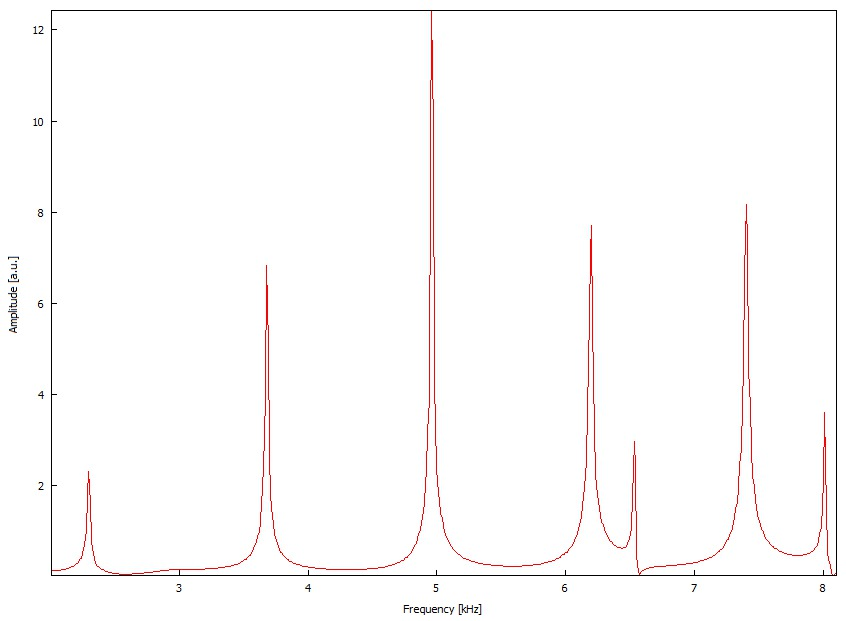
\includegraphics[width=0.4\textwidth]{2.3.2/Raw50a180.jpg}
			\label{Raw50a180}}
		\caption{Fig \protect\subref{LinRegime} shows the linear regime of the frequency spectrum with maximum attenuation. Fig \protect\subref{Raw50a180} shows that same frequency range with a half-attenuated signal.}
		\label{freqSpec}
	\end{figure}
	
	
	
	
	\subsection{Measuring Spherical Cavity Resonances with the Computer}
	In this section, we used the sound card in the computer to both generate and measure the resonances within the cavity. We set the attenuator to its highest value ($10$) to protect the sound card. The sound card output is connected to the Quantum Analogs \emph{Sine Wave Input} and to channel 1 of the oscilloscope. The \emph{AC Monitor} from the Quantum Analogs device is connected to the microphone input on the sound card and to channel 2 of the oscilloscope. 
	

	
%	Starting with $\alpha = 180 \deg$ and a step size of $10$ Hz, we sweep from $2$ to $8.1$ kHz and record the amplitude. We repeat this process for $\alpha = 40\deg, 20\deg$ and $0\deg$. We resolved the peak around $5$ kHz by decreasing the step size to from $10$ Hz to $0.5$ Hz. \red{figure references} 
	
	\subsection{Potential Problems}
	One potential problem is the phenomena of \emph{cross talk} when taking measurements with the computer. When the computer is being used to take measurements, it is simultaneously supplying the signal into the cavity. Cross talk occurs when the signal being sent into the cavity crosses into the line coming out of the cavity. Hence the input and output channels of the computer ``talk'' to each other. 
	
	One surefire way to eliminate cross talk is to simply use a higher quality sound card. If this is not an option, you will need to resort to adjusting the amplitude of the output, attenuation, and microphone sensitivities to minimize cross talk.
	
	
	
	
\section{Results and Analysis}
	
	\subsection{Determining Resonant Frequencies}
	Once we restricted our attention to the linear regime, see \figref{Raw50a180}, we began isolating the resonant frequencies using the oscilloscope. On the oscilloscope, a resonance will appear as in increase in the amplitude orders of magnitude larger than the characteristic scale of the signal. Near a resonance, we fine tune the frequency in increments of $1$ Hz until the amplitude is maximized. It is important to note that denominations smaller than $1$ Hz are not discernible on the oscilloscope due to the limited resolution of the screen. A table summarizing the resonant frequencies and their nodal angles is provided in \figref{freqTable}. For a full summary of the acoustic amplitude vs polar angle measurements for all resonant frequencies, see \cref{2291Table,3679Table,4962Table,6202Table,7409Table} in the appendix. For the corresponding graphs of acoustic pressure versus polar angle, see \cref{2291Graph,3679Graph,4962Graph,6202Graph,7409Graph}.
	
	\begin{table}[H]
		\captionsetup{justification = centering}
		\centering
		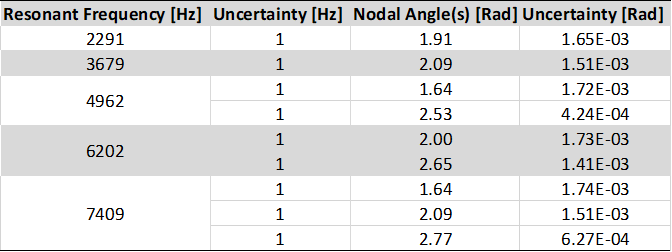
\includegraphics[width=0.6\textwidth]{Tables/ResTable.png}
		\caption{Table of measured resonant frequencies, nodal angles, and associated uncertainties.}
		\label{freqTable}
	\end{table}

	\subsection{Spectrum Response to Varying $\alpha$}
	Once we obtained the frequency spectrum in the linear regime of the signal, we varied $\alpha$ to observe how the spectrum changes as a function of cavity angle. Below are a series of measurements which show how the spectra changes as the cavity angle decreases from $40\deg$ to $0\deg$.
	
	\begin{figure}[H]
		\centering
		\subfloat[Spectrum for $\alpha = 40\deg$]{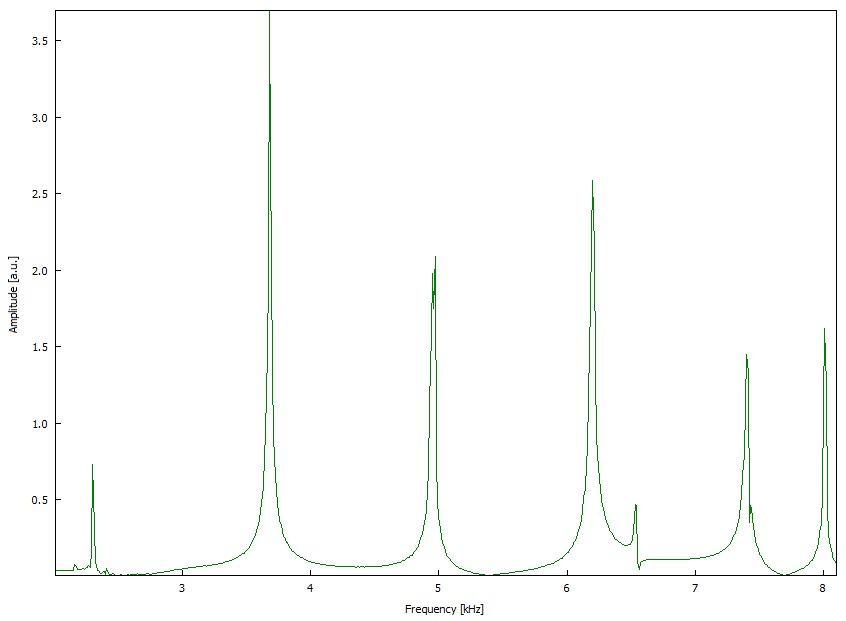
\includegraphics[width=0.3\textwidth ]{2.3.2/Raw50a40.jpg}}
		\quad
		\subfloat[Spectrum for $\alpha = 20\deg$]{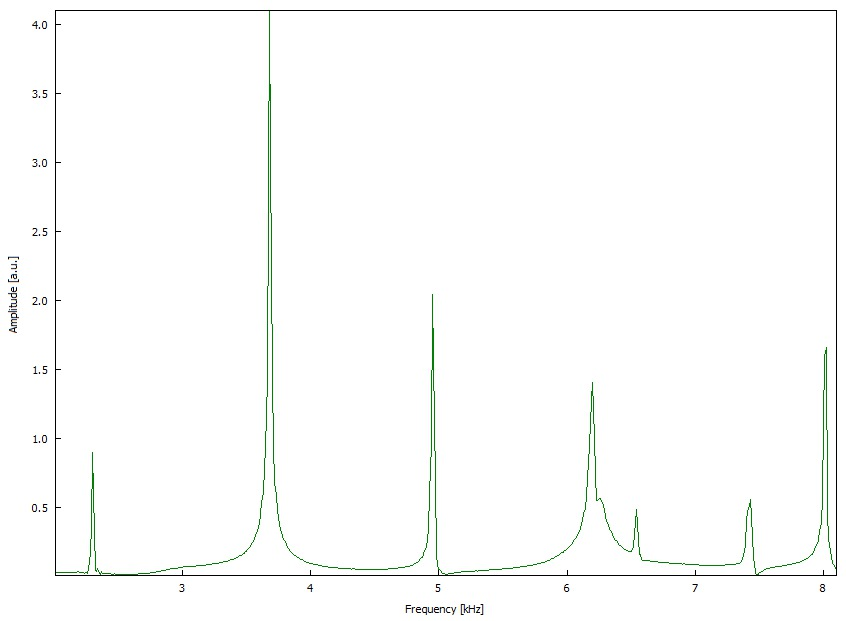
\includegraphics[width=0.3\textwidth]{2.3.2/Raw50a20.jpg}}
		\quad
		\subfloat[Spectrum for $\alpha = 0\deg$]{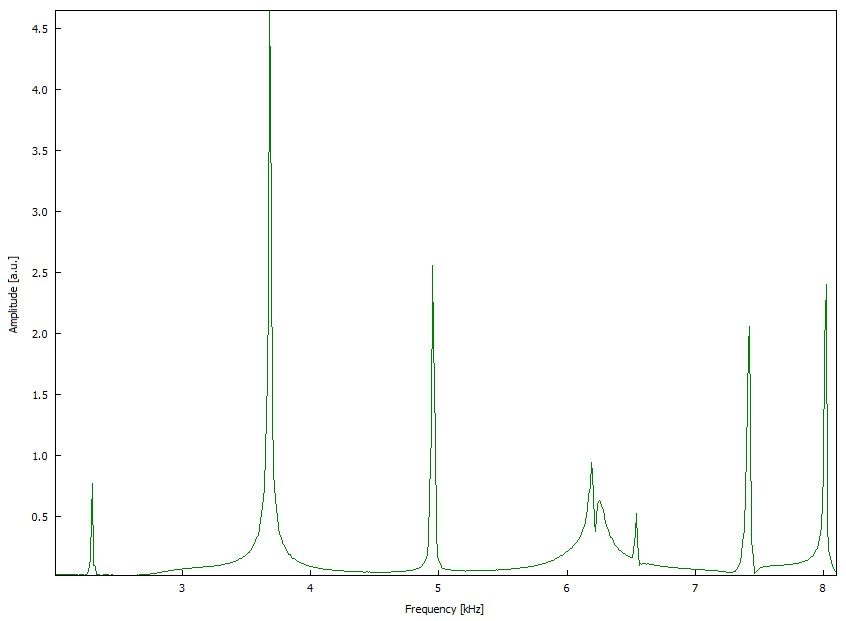
\includegraphics[width=0.3\textwidth]{2.3.2/Raw50a0.jpg}}
		\caption{Graphs showing the spectrum as we vary the cavity angle $\alpha$ from $40\deg$ to $0\deg$. We can see that as $\alpha$ decreases, the resonance at $\approx6$ kHz drops off.}
		\label{angleSpectra}
	\end{figure}

	We can see that as the cavity angle approaches $0\deg$, the resonance at $\approx6$ kHz starts large and drops off while the resonance at $\approx7.5$ kHz starts large, drops off, and then increases. This is due to the angular dependence of the spherical harmonics and specifically, the Legendre Polynomials. As the order of the polynomial increases, antinodes form closer and closer to $\cos(\theta) = 1$. In other words, the behavior of higher frequency resonances is more erratic near angles close to $\cos(\theta) = 1$, see the Legendre polynomials in \cref{L1,L2,L3,L4,L5} in the appendix. So as we vary the cavity angle from $40\deg$ to $0\deg$, some Legendre polynomials decrease while others increase.


%	\begin{figure}[H]
%		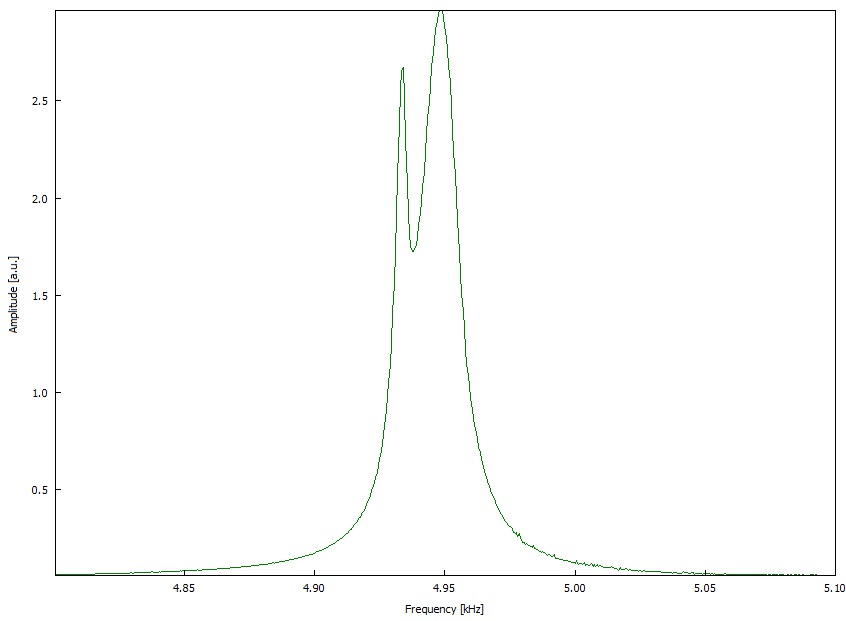
\includegraphics[width=0.3\textwidth]{2.3.2./Raw50a0res.jpg}
%		\caption{Hi resolution spectrum\\ at the $5$ kHz resonance}
%		\label{hiRes5K}
%	\end{figure}
	
		
	
	\subsection{Determining $\ell$ values for each Resonance}
	Once we have isolated the resonant frequencies, we seek to determine what $\ell$ value they correspond to. We will present two ways to achieve this. First, we compare graphs of the acoustic amplitude vs $\cos(\theta)$ to the Legendre polynomials. Since the acoustic amplitude is the analog of the wavefunction, the shape of the graphs should match. Second, we compare the polar plots of acoustic amplitude vs polar angle to the spherical harmonics. This time, the polar plots should match the shapes of the spherical harmonics.
	
	We begin by noting that for any quantum mechanical system, the wavefunction $\psi$ is an inherently imaginary quantity. We can only ever observe real quantities however. To extract any observable quantity from the wavefunction, we must take its amplitude $|\psi|^2$. For the Hydrogen atom, the wavefunction is proportional to the spherical harmonics $\Ylm{\ell}{m}$ and thus also proportional to the Legendre polynomials $\mathrm{P}_\ell(\cos(\theta))$. So, the graphs of acoustic amplitude vs $\cos(\theta)$ should match the magnitude of the Legendre polynomials from the amplitude of the wavefunction $|\mathrm{P}_\ell(\cos(\theta))|^2$. Similarly, polar plots of acoustic amplitude should match the real component of the spherical harmonics.
	

	\subsubsection{Comparison to Legender Polynomials}
	In this section, we determine the $\ell$ value of the $7409$ Hz resonance by comparison to a Legendre polynomial. We present below, a single comparison of acoustic pressure and the corresponding Legendre polynomial. The rest of the comparisons may be found in \cref{legendre1,legendre2,legendre3,legendre4,legendre5} in the Appendix.
	
	\begin{figure}[H]
		\centering
		\subfloat[Caption A]{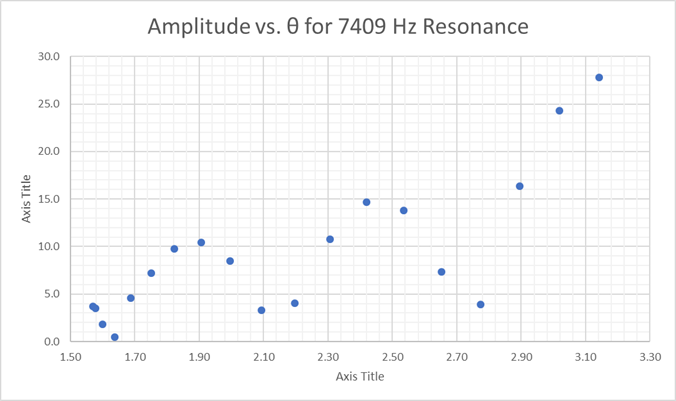
\includegraphics[height=6cm]{Graphs/7409Graph.png}\label{graph1}}
		\qquad
		\subfloat[Caption B]{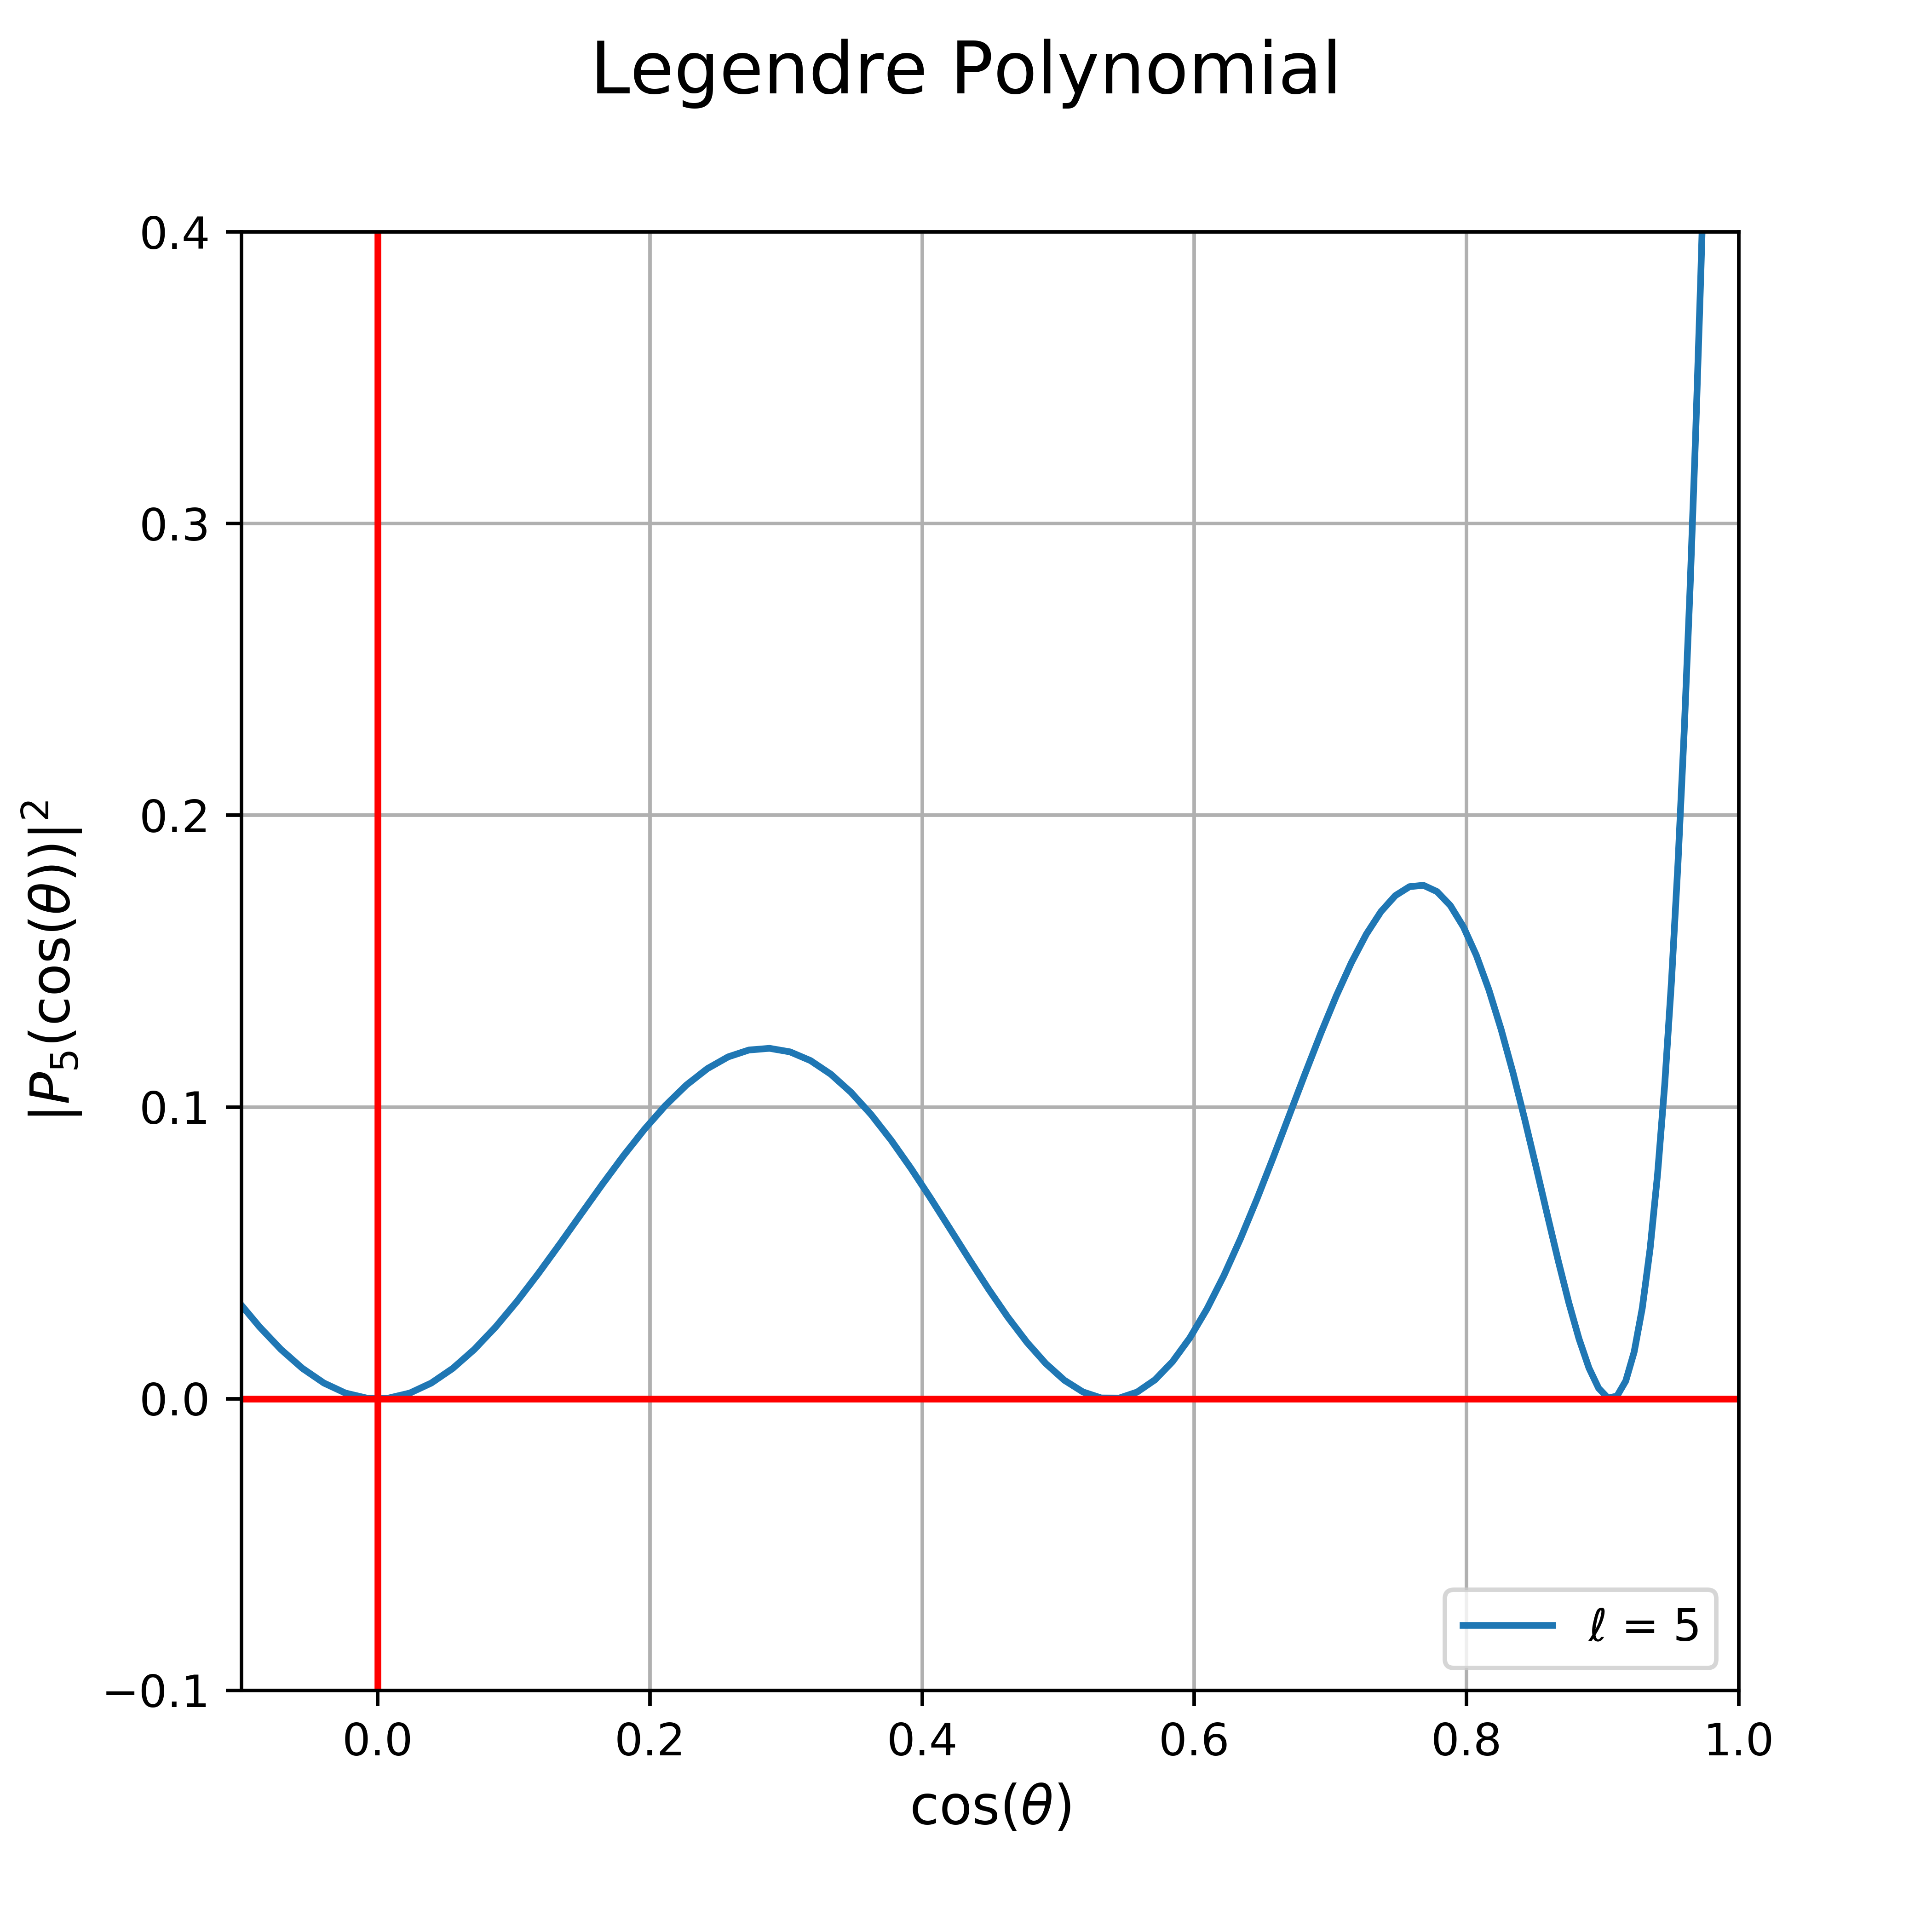
\includegraphics[height=6cm]{Legendre/legendreL5.png}}
		\caption{A qualitative inspection indicates that the resonance at $7409$ Hz corresponds to the $\ell=4$ Legendre polynomial}
		\label{comparison}
	\end{figure}
	
	\pagebreak
	
	The distinguishing features of \figref{graph1} are the starting location at $\cos(\theta) = 0$ and the number of nodes. Since the amplitude starts relatively close to zero, and has $3$ nodes total, a qualitative comparison suggests that the $7409$ Hz resonance corresponds to $\ell=5$.
	
	
	\begin{wraptable}[14]{l}{0.4\textwidth}
		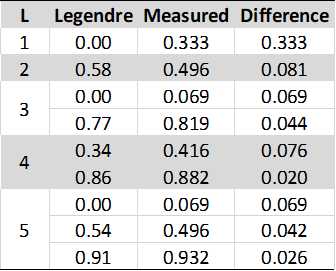
\includegraphics[width=0.35\textwidth]{Tables/LegendreTable.png}
		\caption{Table of numerically calculated zeros of the Legendre polynomials and the measured zeros.}
		\label{legendreTable}
	\end{wraptable}
	

	We may further compare the location of the zeros we measured against the zeros of the Legendre polynomials. I calculated the zeros numerically in Python and summarize the analysis in \cref{legendreTable}. The ``L'' column denotes the $\ell$ value of the Legendre polynomial. The ``Legendre'' column denotes the value of the zero. The column labeled ``Measured'' contains our measured zeros and the ``Difference'' column is simply the difference between the actual value and our measured value.


	\subsubsection{Comparison to Spherical Harmonics}
	To make a comparison to the spherical harmonics, we began mapping out how the acoustic amplitude varries as a function of cavity angle at each resonance. To begin, we set the angle on the cavity to $\alpha = 180 \deg$ and record the acoustic amplitude using the ``Measure wavefunction'' button on the computer. We then decrease $\alpha$ from $180 \deg$ to $0 \deg$ in increments of $\alpha = 10\deg$. Initially, we used increments of $5\deg$ but the amplitude variation was so small, we were unable to determine if the change was due to an actual change in amplitude, or do to statistical fluctuations. 
	
	Once we obtained the polar amplitude plots, we can simply compare them qualitatively to the real component of the spherical harmonics. \figref{SphCompare} below shows one such comparison. The remaining polar acoustic amplitude plots can be seen in \figref{polarGraphs} and their corresponding spherical harmonics in \figref{sphereHarm}. From this qualitative comparison, it is possible to determine the $\ell$ value for each resonance.
	
%	A second way to determine the $\ell$ value for the resonances relies on plotting the acoustic amplitude against polar angle and comparing it to the spherical harmonics. Again, since the spherical harmonics are imaginary, we plot the real component. 
	
%	\vskip 2cm
	
	\begin{figure}[H]
		\centering
		\subfloat[Acoustic Amplitude vs. polar angle]{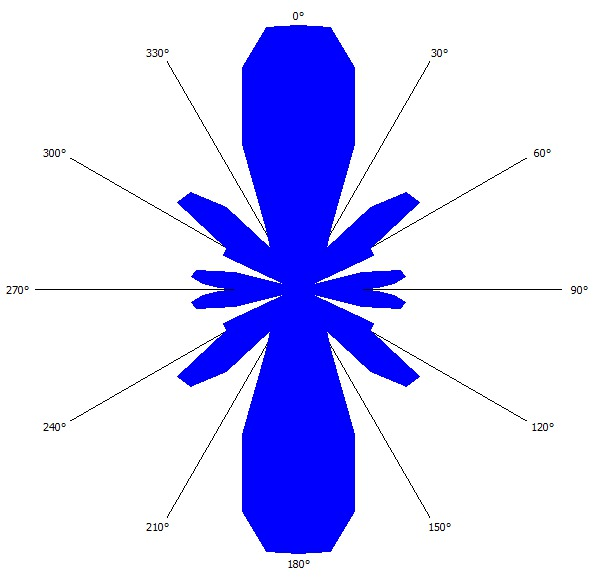
\includegraphics[width=0.3\textwidth]{2.3.2/F7409.jpg}}
		\qquad
		\subfloat[Spherical harmonic corresponding to $\Ylm{0}{5}$]{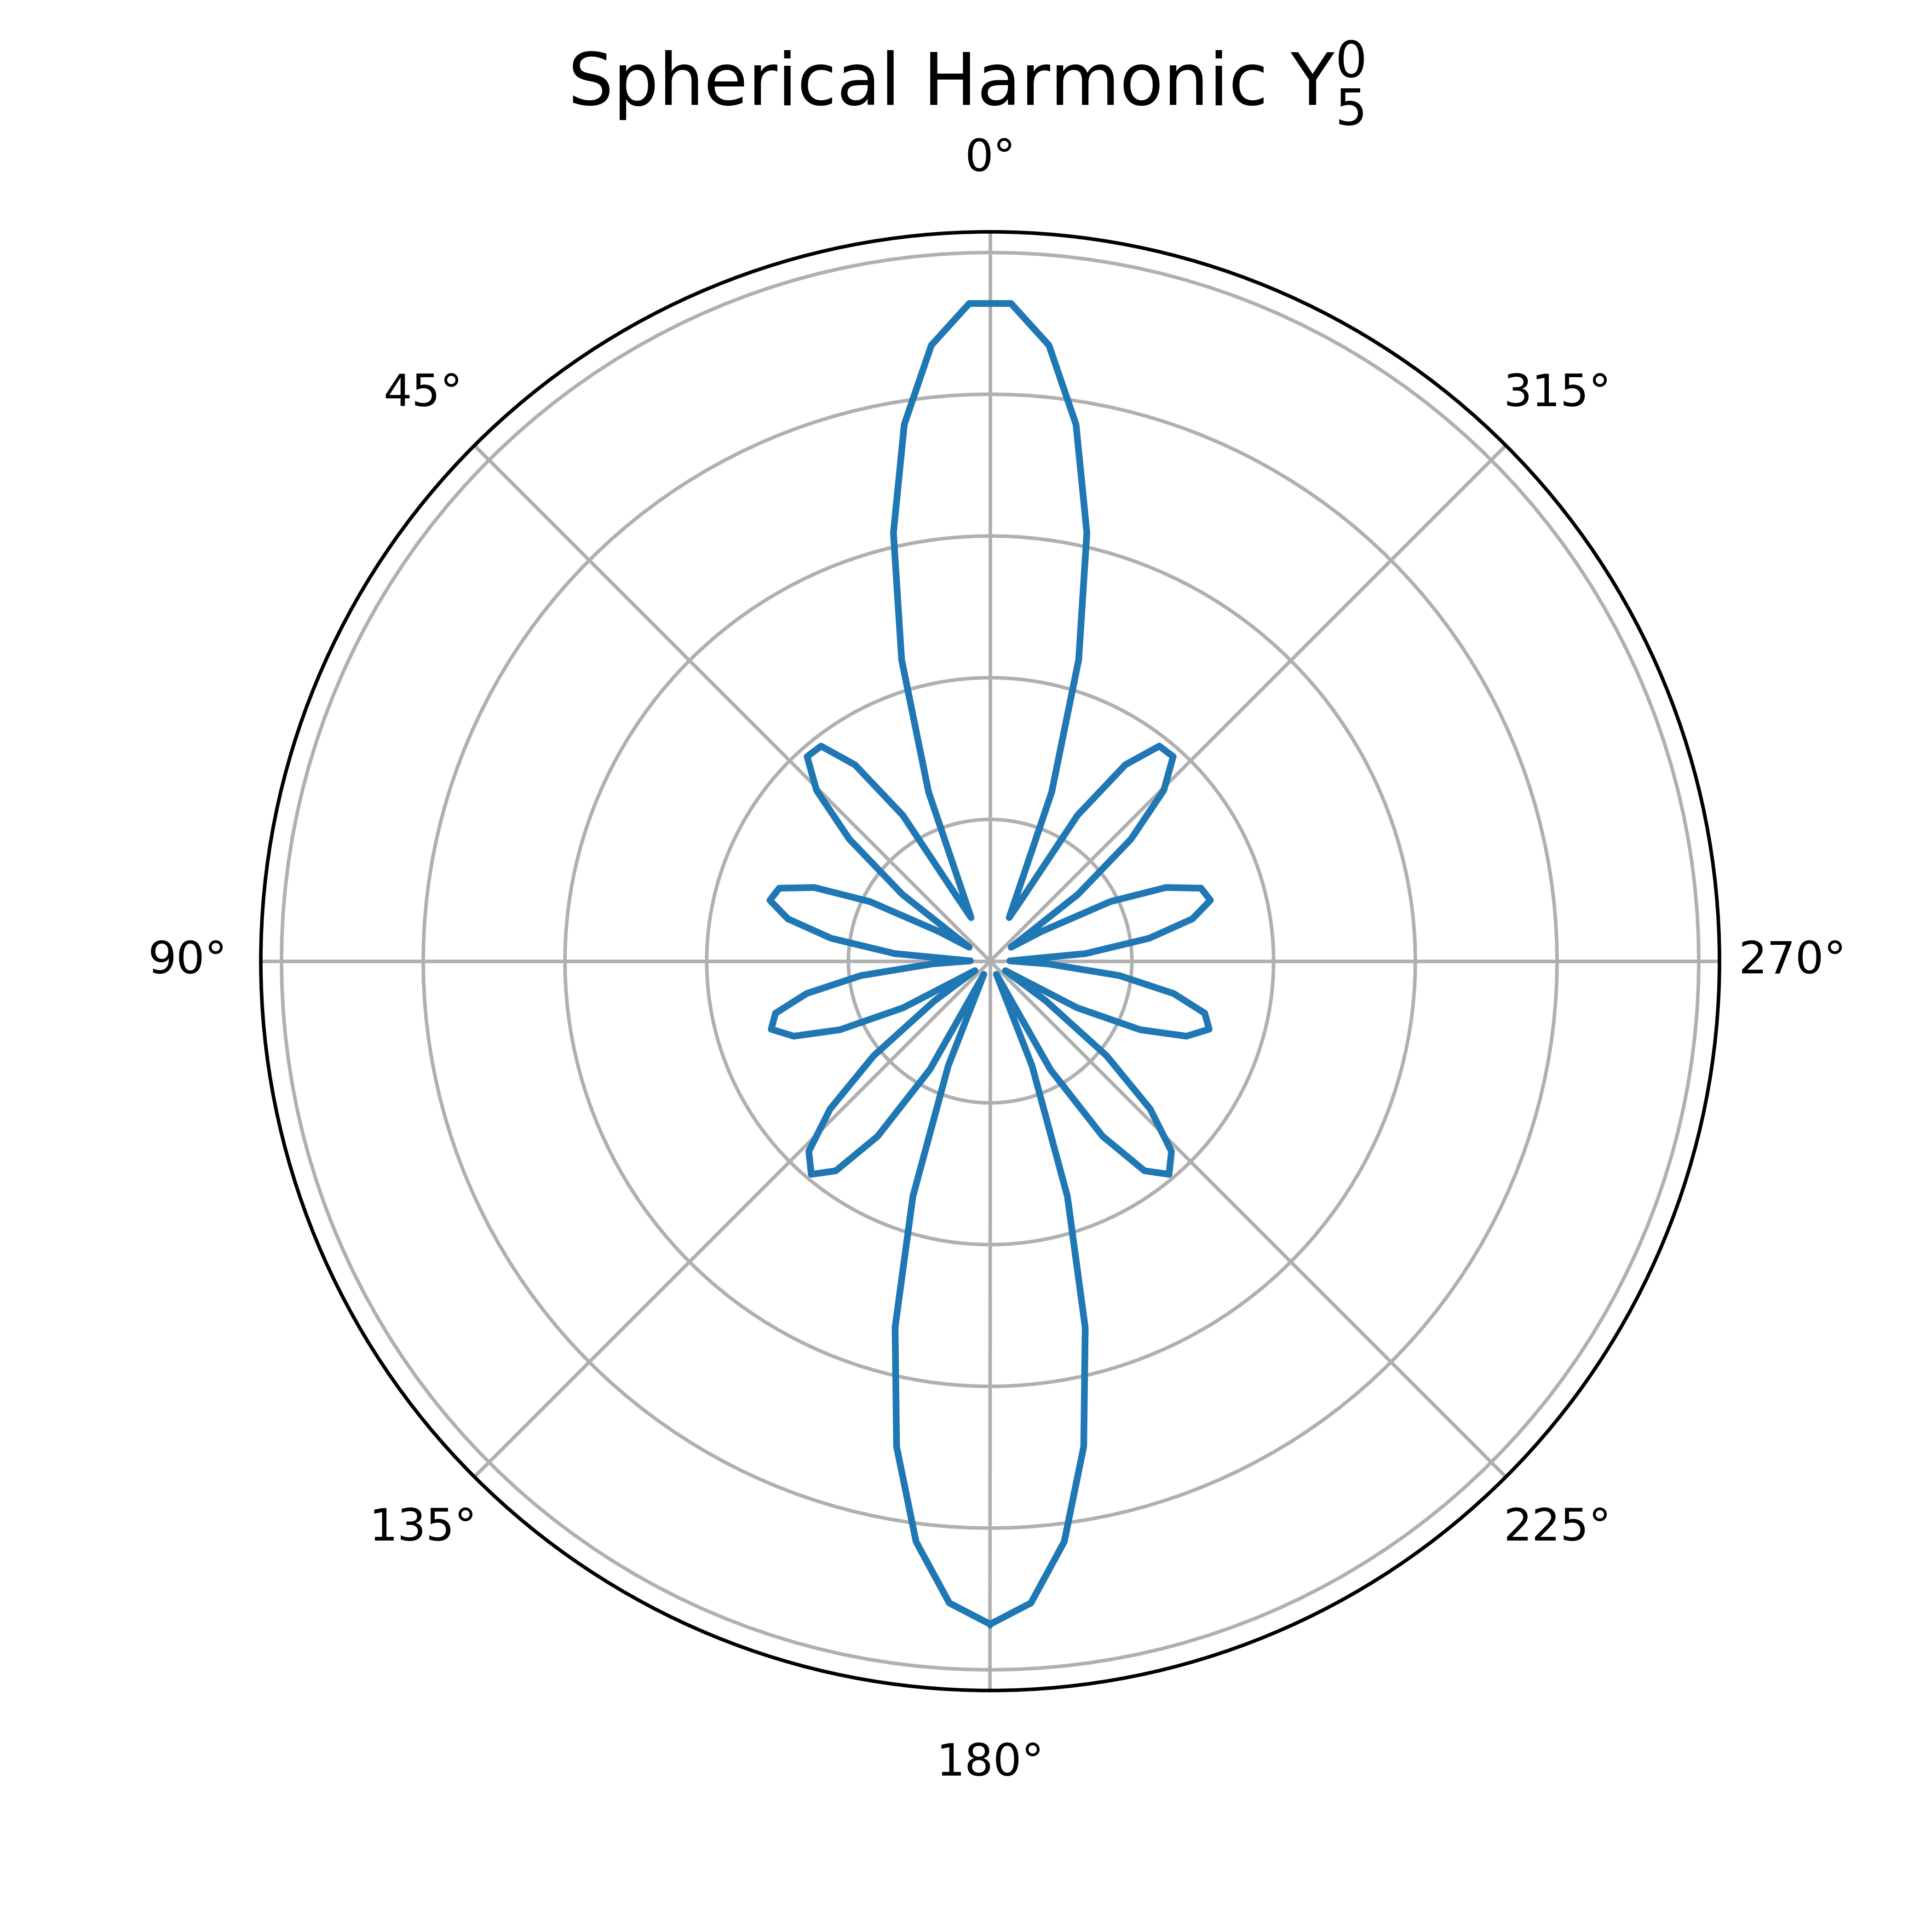
\includegraphics[width=0.3\textwidth]{SphHarm/SphHarmL5M0.png}}
		\caption{A comparison between the acoustic amplitude as a function of cavity angle and the corresponding spherical harmonic}
		\label{SphCompare}
	\end{figure}
	
	\subsection{$\ell=1$ Degeneracy}
	Recall that a quantum system with angular momentum $\ell$ has a $(2\ell+1)$ degeneracy of states. It is possible to resolve these degeneracies by breaking the spherical symmetry of the cavity. We achieve this by introducing spacing rings into the cavity, simulating a magnetic field which gives a quantization axis to the system. This symmetry-breaking process is visualized in \figref{degenResolution} where we can observe the peak splitting as the spacing is increased. The lower frequency which emerges is the $m=0$ state and the higher frequency is degenerate for $m=\pm1$.
	
	\begin{figure}[H]
		\centering
		\subfloat[$\ell=1$ resnonance with spherical symmetry.]{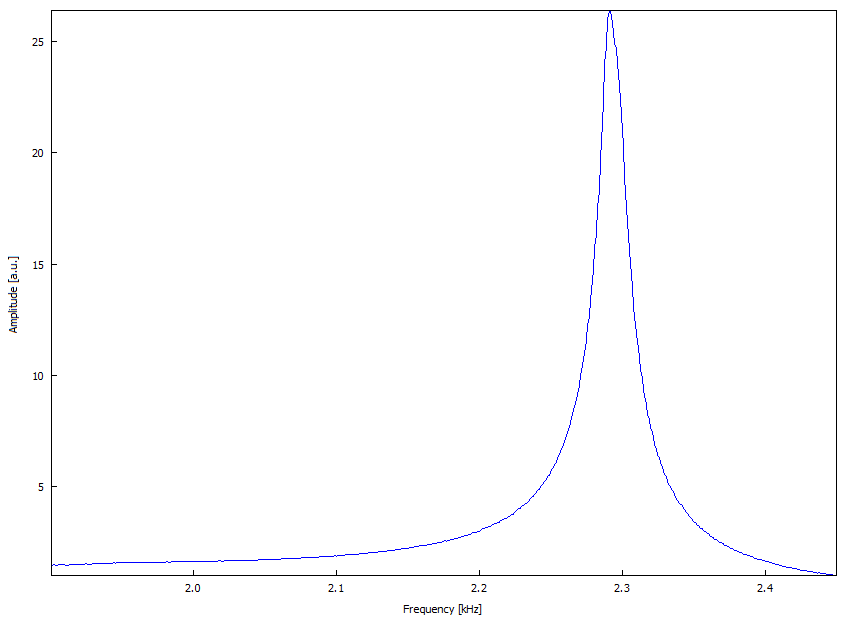
\includegraphics[width=0.4\textwidth]{Day4/L1ResonanceSpectrum.png}\label{degenResolutionSphere}}
		\qquad
		\subfloat[$\ell=1$ resnonance with $3$ mm spacing.]{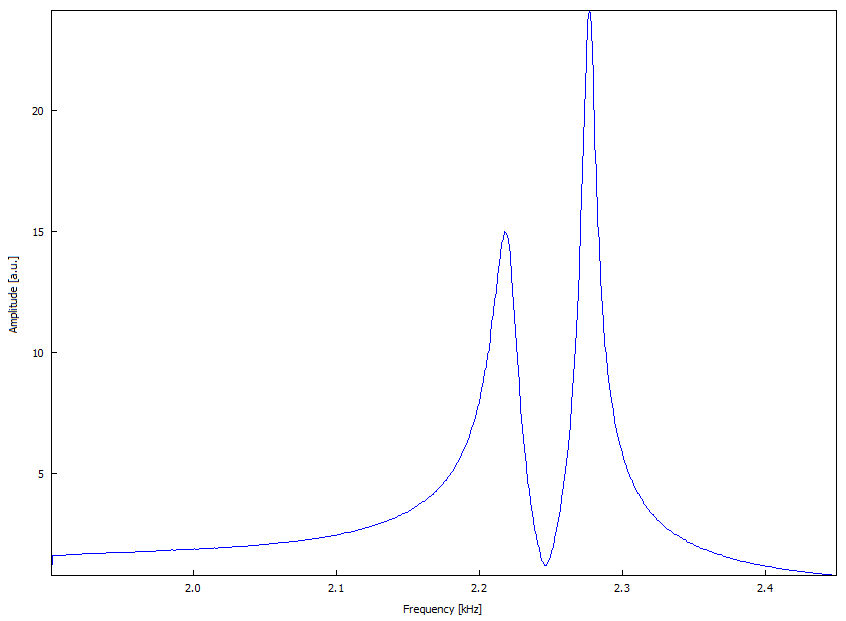
\includegraphics[width=0.4\textwidth]{Day4/L1ResonanceSpectrum3mm.png}\label{degenResolution3mm}}
		\\
		\subfloat[$\ell=1$ resnonance with $6$ mm spacing.]{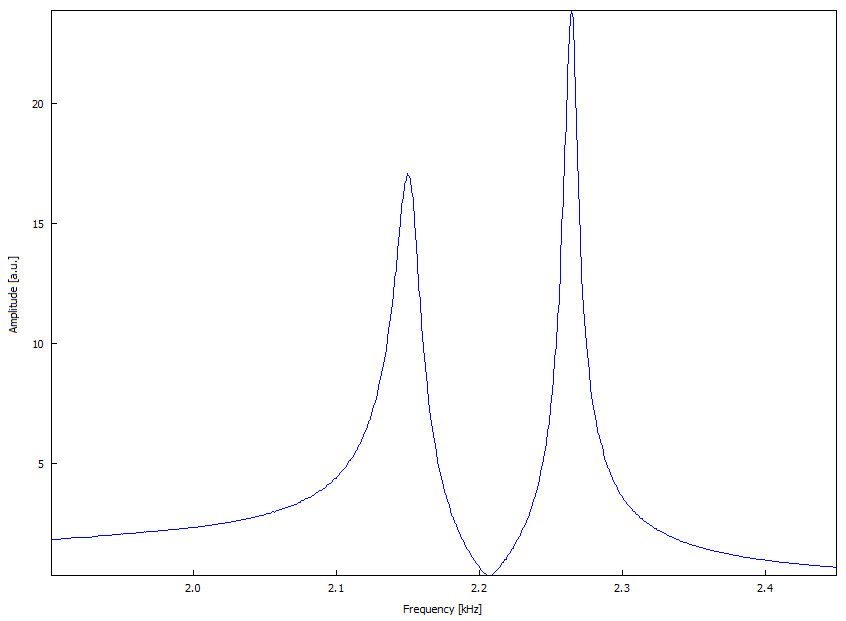
\includegraphics[width=0.4\textwidth]{Day4/L1ResonanceSpectrum6mm.png}\label{degenResolution6mm}}
		\qquad
		\subfloat[$\ell=1$ resnonance with $9$ mm spacing]{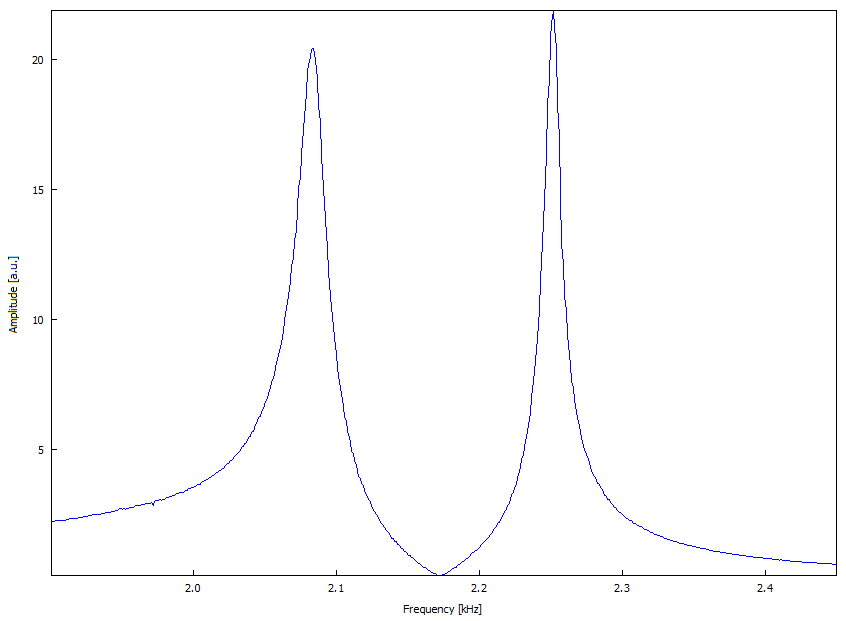
\includegraphics[width=0.4\textwidth]{Day4/L1ResonanceSpectrum9mm.png}\label{degenResolution9mm}}
		\caption{We can see as we break the spherical symmetry by introducing spacer rings to the cavity, the degeneracy in the $\ell=1$ resonance is lifted and we can resolve the $\ell = 0$ and $\ell = \pm1$ peaks.}
		\label{degenResolution}
	\end{figure}



	We may further investigate by examining polar plots of the amplitude to determine the magnetic quantum number $m$. \figref{9mmPolarliftedDegeneracy} shows the polar graphs of acoustic pressure vs. azimuthal angle $\varphi$ for a cavity with the maximal separation of $9$ mm. Polar amplitude graphs for the $3$ mm and $6$ mm spacing rings can be seen in \figref{3mmliftedDegeneracy} and \figref{6mmliftedDegeneracy} in the appendix.
	
	\begin{figure}[H]
		\centering
		\subfloat[$\ell=1$, $m=0$ orbital with 9mm spacing.]{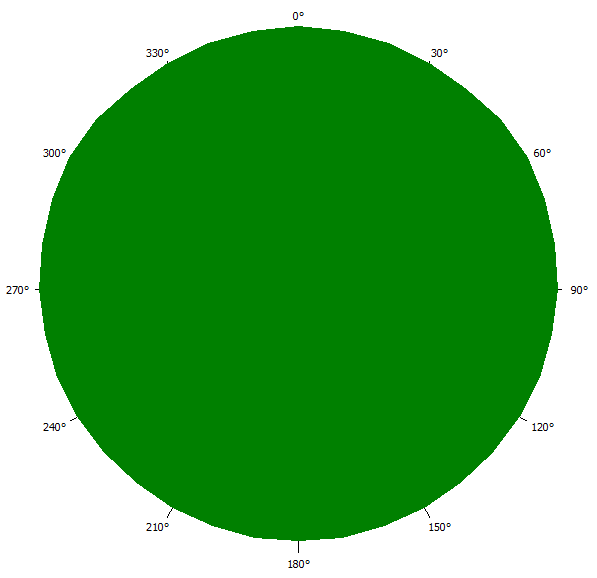
\includegraphics[width=0.3\textwidth]{Day4/L19mmPolar2084_806.png}\label{liftedDegeneracyL1M0}}
		\qquad
		\subfloat[$\ell=1$, $m=\pm1$ orbital with 9mm spacing.]{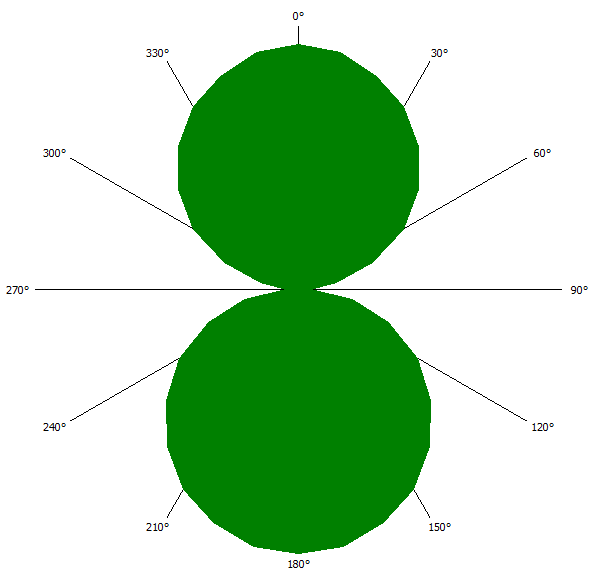
\includegraphics[width=0.3\textwidth]{Day4/L19mmPolar2251_140.png}\label{liftedDegeneracyL1M1}}			
%		\caption{Acoustic amplitude vs azimuthal angle $(\varphi)$ for polar angle $(\theta=0)$ cavity with broken symmetry. We can see that the degeneracy for the $\ell=1$ resonance is partially lifted. The $m=\pm1$ states are still degenerate since they are symmetric with respect to the azimuthal angle phi.}
		\caption{Projections of acoustic amplitude vs azimuthal angle $(\varphi)$ onto the $\theta=0$ plane. Angle markings indicate the azimuthal angle $\varphi$.}
		\label{9mmPolarliftedDegeneracy}		
	\end{figure}

	We can resolve the $\ell=1$ state into $m=0$ and $m=\pm1$. The $m=\pm1$ states are still degenerate because they are symmetric under rotations in the azimuthal angle $\varphi$. This can be seen in the $\varphi=0$ projections of the spherical harmonics in \figref{L1M1Comparison}. The $\varphi=0$ projection of $\Ylm{1}{0}$, as seen in \figref{sphHarml1m0}, is exactly the shape of the orbital we measured in \figref{liftedDegeneracyL1M0}. Similarly, the shape of the $\varphi=0$ projection of $\Ylm{1}{1}$ in \figref{sphHarml1m1} is symmetric in $\varphi$ and matches the $\theta=0$ projection of \figref{liftedDegeneracyL1M1}.

	\begin{figure}[H]
		\centering
		\subfloat[Projection of $\Ylm{1}{0}$ onto the $\varphi = 0$ plane.]{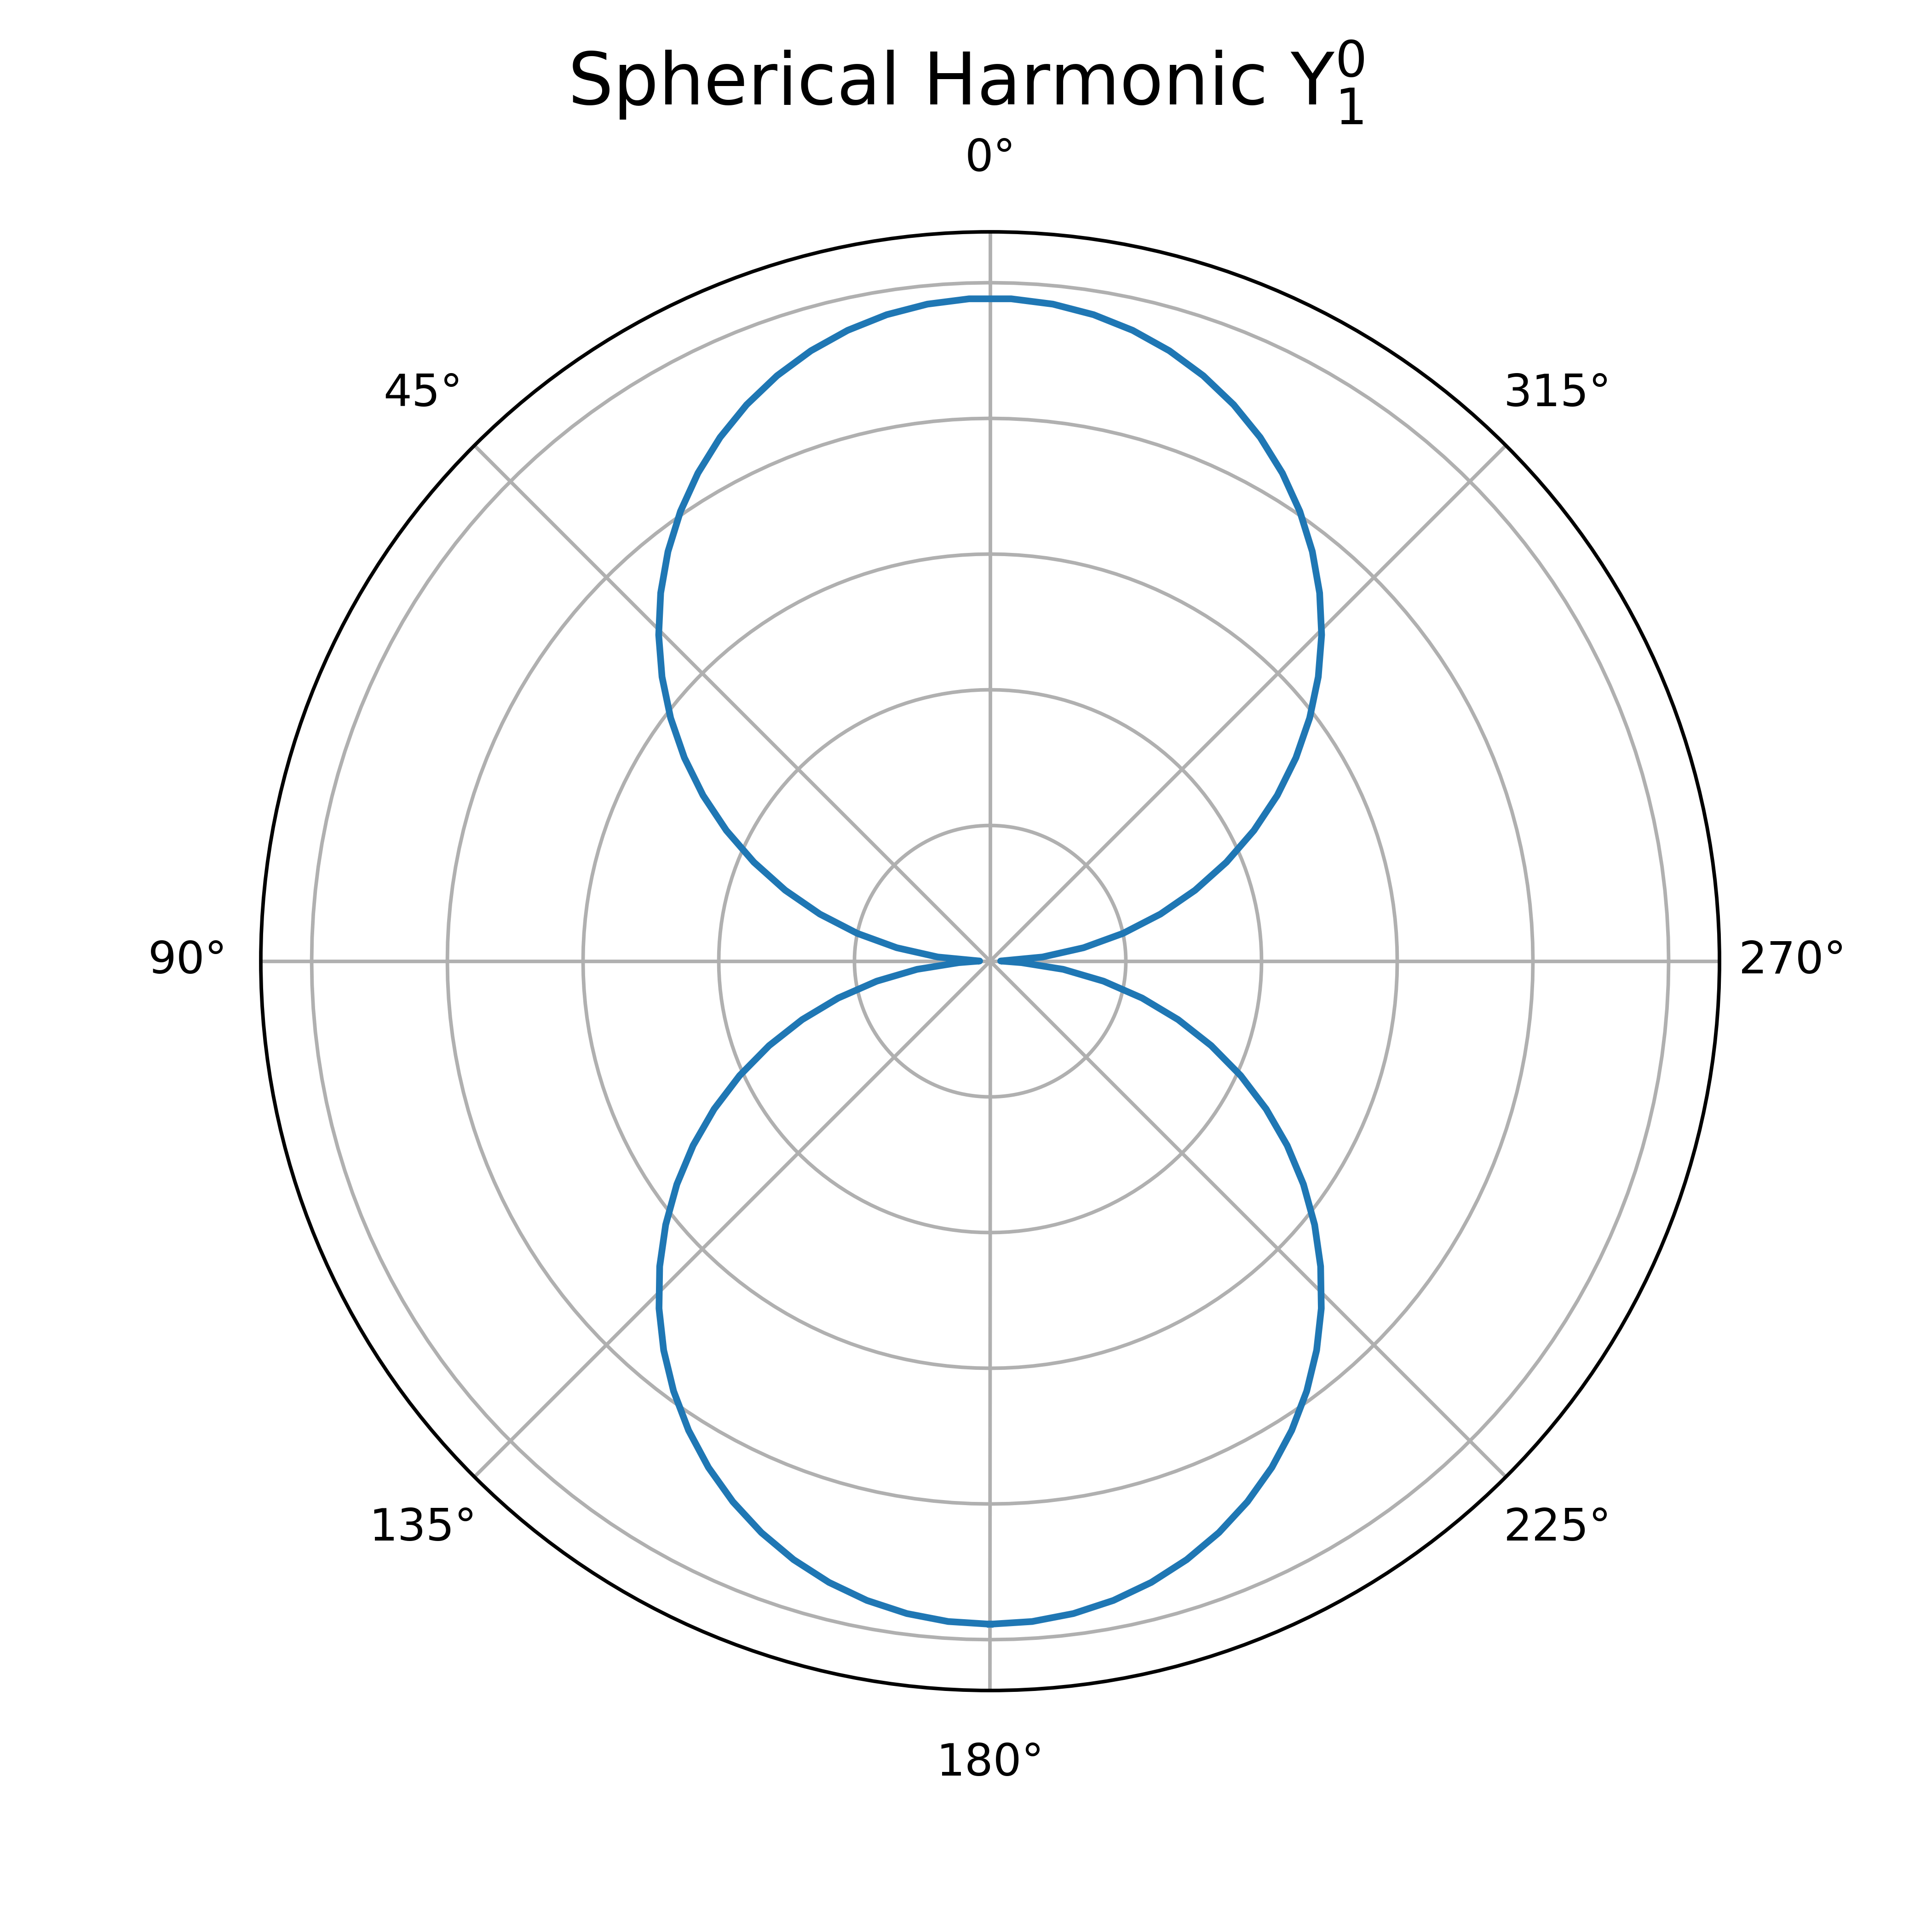
\includegraphics[width=0.3\textwidth]{SphHarm/SphHarmL1M0.png}\label{sphHarml1m0}}
		\qquad
		\subfloat[Projection of $\Ylm{1}{1}$ onto the $\varphi = 0$ plane.]{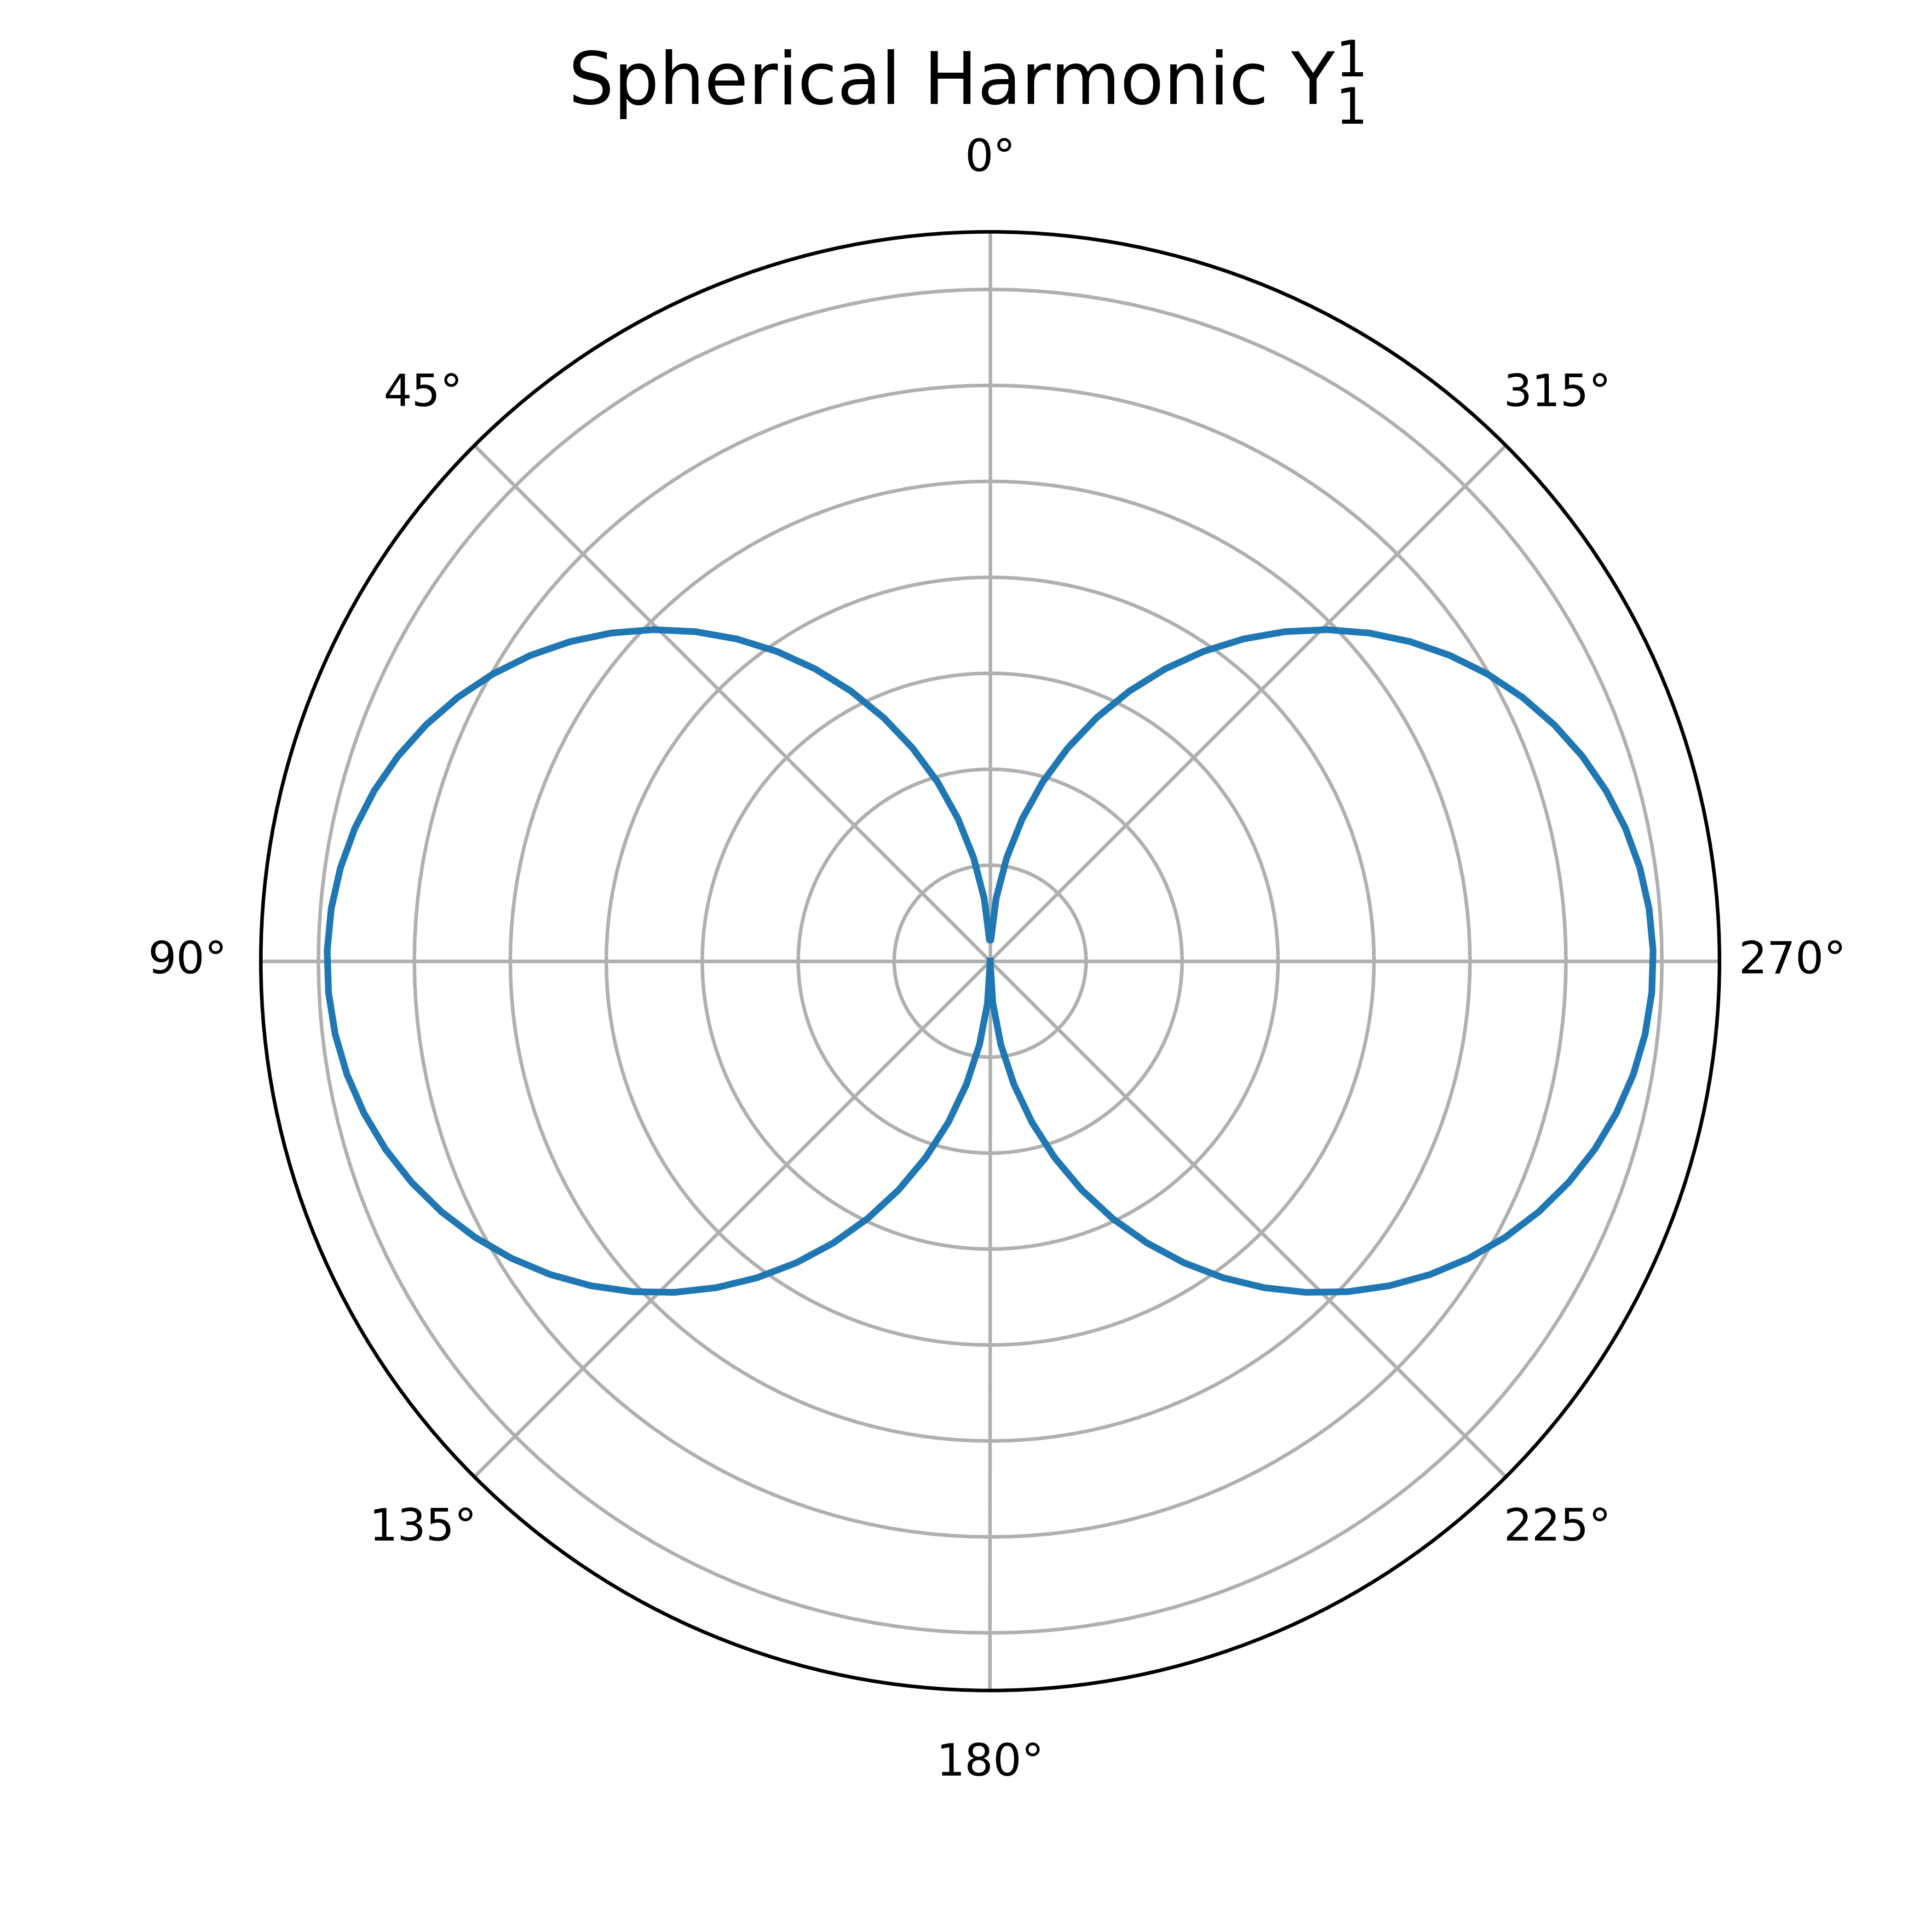
\includegraphics[width=0.3\textwidth]{SphHarm/SphHarmL1M1.png}\label{sphHarml1m1}}
		\caption{Projections of the spherical harmonics onto the $\varphi=0$ plane. Angle markings indicate polar angle $\theta$.}
		\label{L1M1Comparison}
	\end{figure}


\redline

\subsection{Phase Measurements}
\red{TO DO}


\begin{figure}[H]
	\captionsetup{justification = centering}
	\centering
	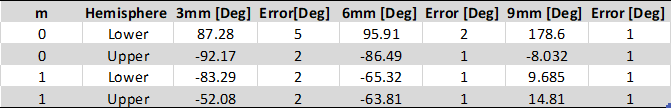
\includegraphics[width=0.8\textwidth]{Tables/PhaseMeasurements.png}
	\caption{Table of measured phases for top and bottom hemispheres for all spacer rings}
	\label{phaseTable}
\end{figure}





\section{Conclusion}

	\subsection{Achievements}
	In this experiment, we successfully captured the angular dependence of the Hydrogen wavefunction with a standing pressure wave inside a spherical cavity. We generated spherical harmonics for various angular momenta values. Further, we simulated the Zeeaman effect and achieved partial energy level splitting in the $\ell=1$ state. 

	\subsection{Future Improvements}
	Throughout this experiment, the microphone was extremely sensitive to any noise and even vibrations in the room, chairs moving, the lab bench being bumped, doors closing, etc... One improvement to this experiment is to perform it in an isolated room on a sand table which dampens vibrations from the environment.
	
%%Appendix A


\section{Appendix}
\label{AppendixA}

All numerical calculations were written and performed in Python.

\subsection{Cavity Angle and Polar Angle Relation}

\begin{figure}[H]
	\centering
	\captionsetup{justification = raggedright}
	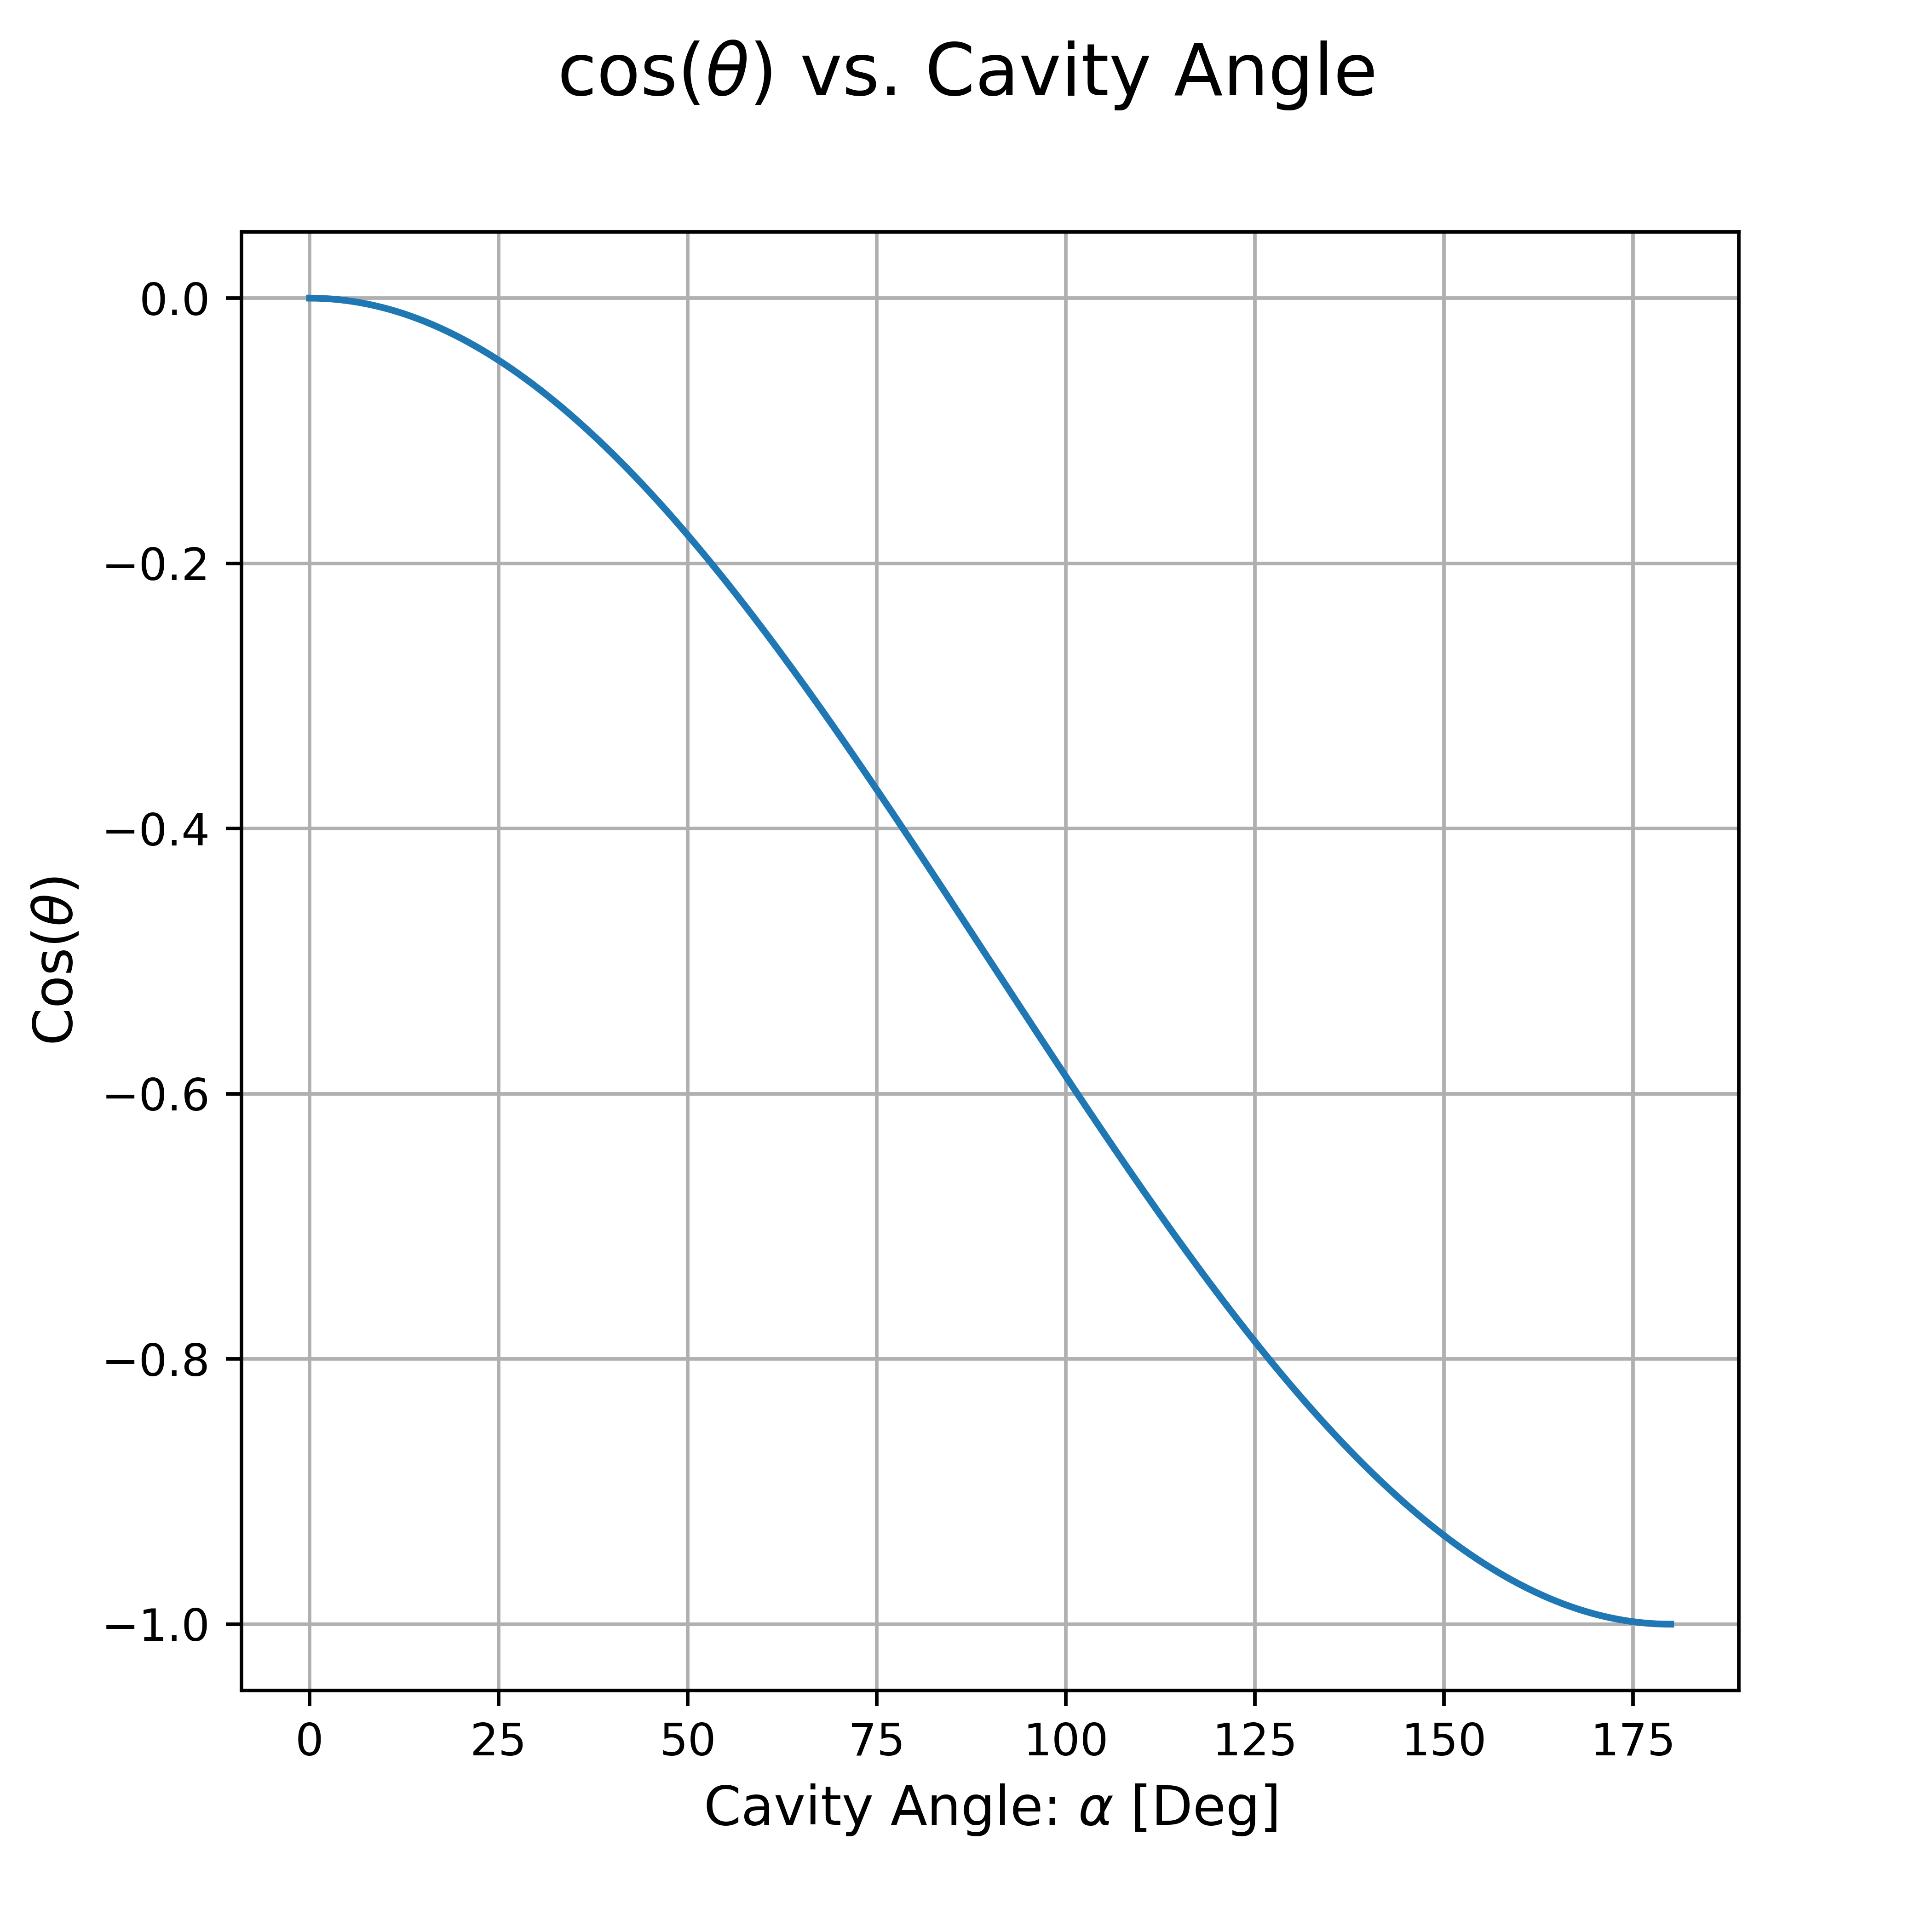
\includegraphics[width=0.4\textwidth]{Graphs/ThetaAlpha.png}
	\caption{Relation between $\cos(\theta)$ and cavity angle $\alpha$ when spherical symmetry is present}
	\label{ThetaAlpha}
\end{figure}


\subsection{Amplitude and Polar Angle Measurement Tables}
For clarity, instead of plotting $\cos(\theta)$ we plot $|\cos(\theta)|$ since cosine is symmetric about $\theta = 0$.

\begin{multicols}{2}
	\begin{table}[H]
		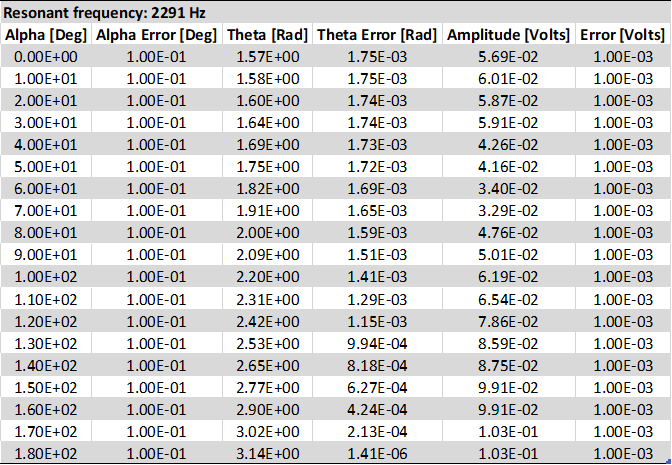
\includegraphics[width=0.45\textwidth]{Tables/2291Table.png}
		\caption{Data table for resonant frequency $2291$ Hz.}
		\label{2291Table}		
	\end{table} 
	\columnbreak
	\begin{figure}[H]
		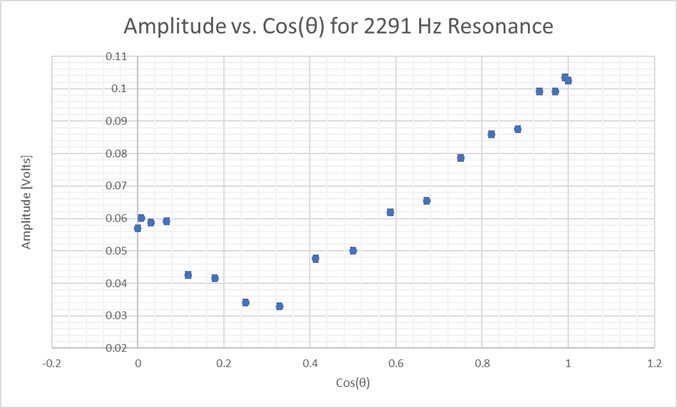
\includegraphics[width=0.45\textwidth]{Graphs/2291Graph.png}
		\caption{Graph of \cref{2291Table}. We can clearly see a single node at $\theta = 1.91$ radians.}
		\label{2291Graph}
	\end{figure}
\end{multicols}

\pagebreak

\begin{multicols}{2}
	\begin{table}[H]
		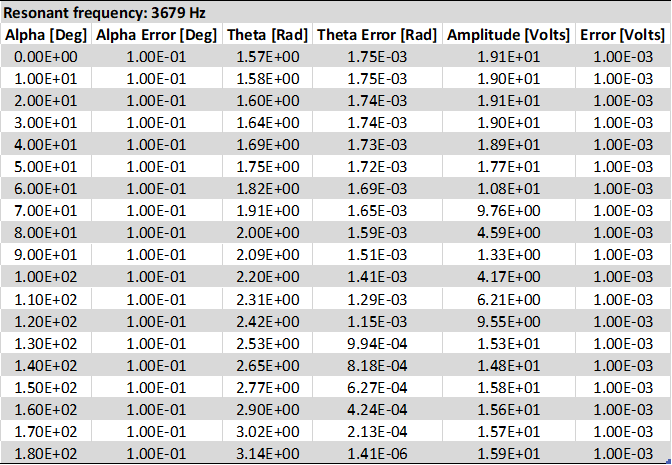
\includegraphics[width=0.45\textwidth]{Tables/3679Table.png}
		\caption{Table showing amplitude vs polar angle for 3679 Hz resonance.}
		\label{3679Table}		
	\end{table} 
	\columnbreak
	\begin{figure}[H]
		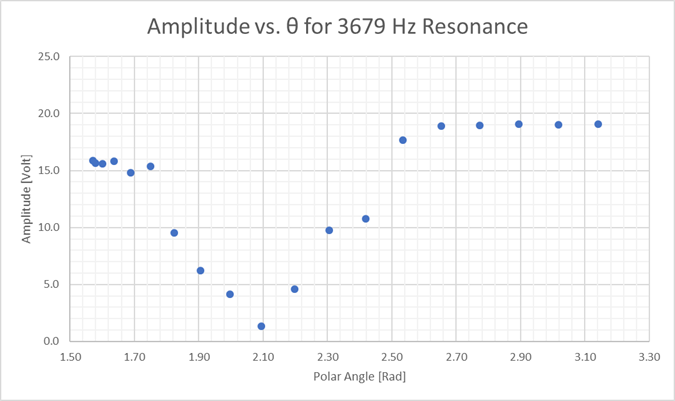
\includegraphics[width=0.45\textwidth]{Graphs/3679Graph.png}
		\caption{Graph of \cref{3679Table}. We can clearly see a single node at $\theta = 2.09$ radians.}
		\label{3679Graph}
	\end{figure}
\end{multicols}



\begin{multicols}{2}	
	\begin{table}[H]
		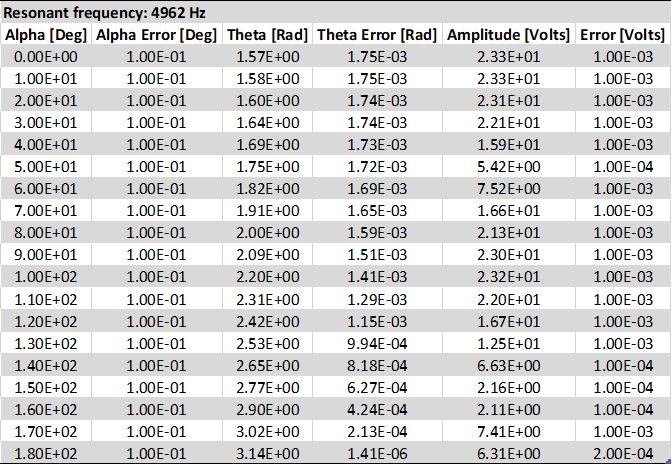
\includegraphics[width=0.45\textwidth]{Tables/4962Table.png}
		\caption{Table showing amplitude vs polar angle for 4926 Hz resonance.}
		\label{4962Table}		
	\end{table}
	\columnbreak
	\begin{figure}[H]
		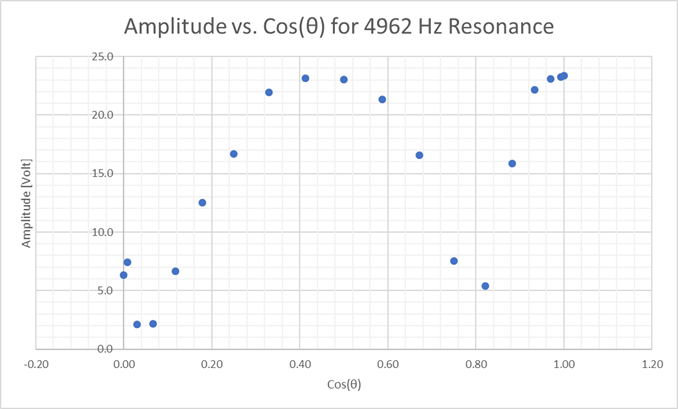
\includegraphics[width=0.45\textwidth]{Graphs/4962Graph.png}
		\caption{Graph of \cref{4962Table}. We can clearly see a single node at $\theta = $ radians.}
		\label{4962Graph}
	\end{figure}
\end{multicols}


\begin{multicols}{2}	
	\begin{table}[H]
		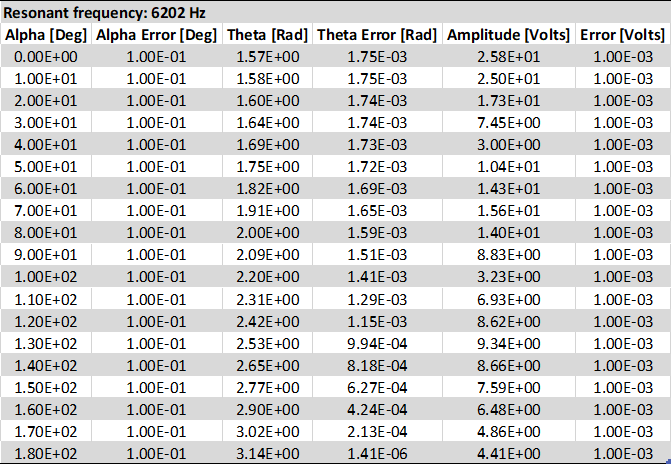
\includegraphics[width=0.45\textwidth]{Tables/6202Table.png}
		\caption{Table showing amplitude vs polar angle for 6202 Hz resonance.}
		\label{6202Table}		
	\end{table}
	\columnbreak
	\begin{figure}[H]
		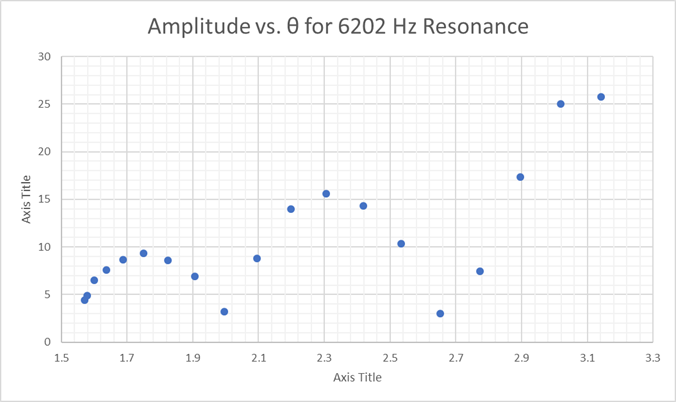
\includegraphics[width=0.45\textwidth]{Graphs/6202Graph.png}
		\caption{Graph of \cref{6202Table}. We can clearly see a single node at $\theta = $ radians.}
		\label{6202Graph}
	\end{figure}
\end{multicols}

\pagebreak

\begin{multicols}{2}	
	\begin{table}[H]
		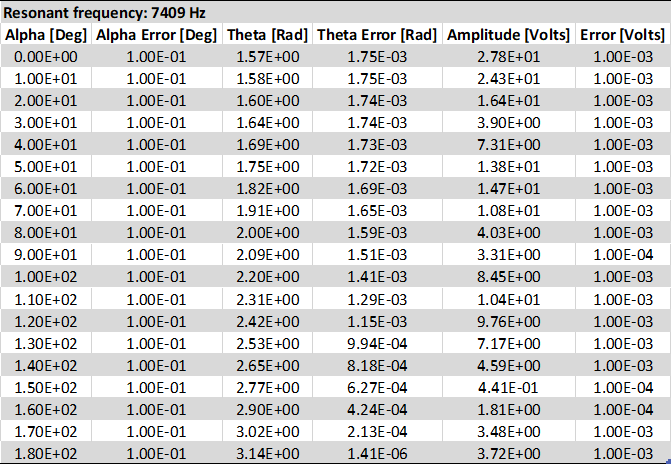
\includegraphics[width=0.45\textwidth]{Tables/7409Table.png}
		\caption{Table showing amplitude vs polar angle for 7409 Hz resonance.}
		\label{7409Table}		
	\end{table}
	\columnbreak
	\begin{figure}[H]
		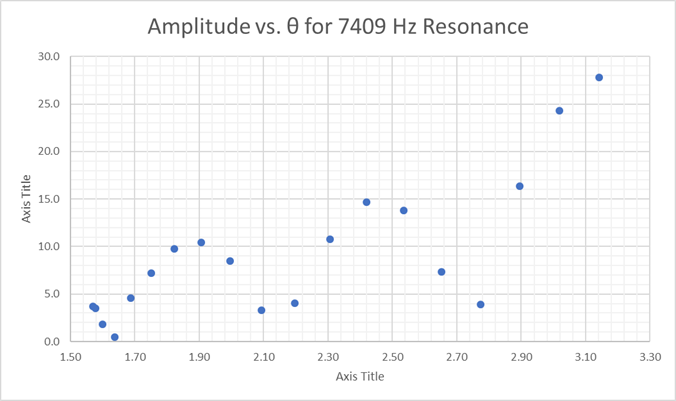
\includegraphics[width=0.45\textwidth]{Graphs/7409Graph.png}
		\caption{Graph of \cref{7409Table}. We can clearly see a single node at $\theta = $ radians.}
		\label{7409Graph}
	\end{figure}
\end{multicols}


\subsection{Legender Polynomial Comparisons}
\begin{figure}[H]
	\centering
	\subfloat[Measured acoustic amplitude plotted against $\cos(\theta)$ for the 2291 Hz resonance]{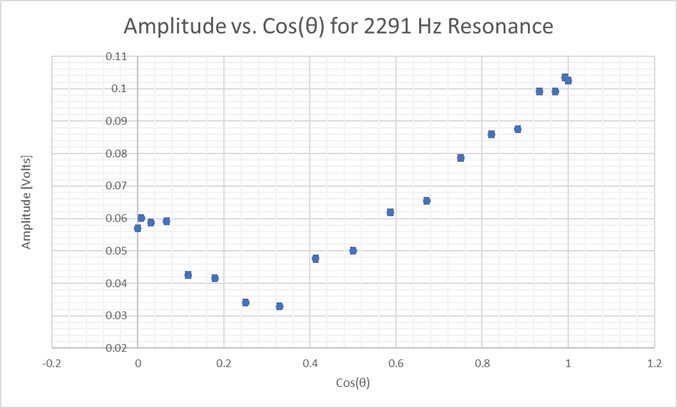
\includegraphics[height=6cm]{Graphs/2291Graph.png}}
	\qquad
	\subfloat[Legendre polynomial $|\mathrm{P}_1|^2$]{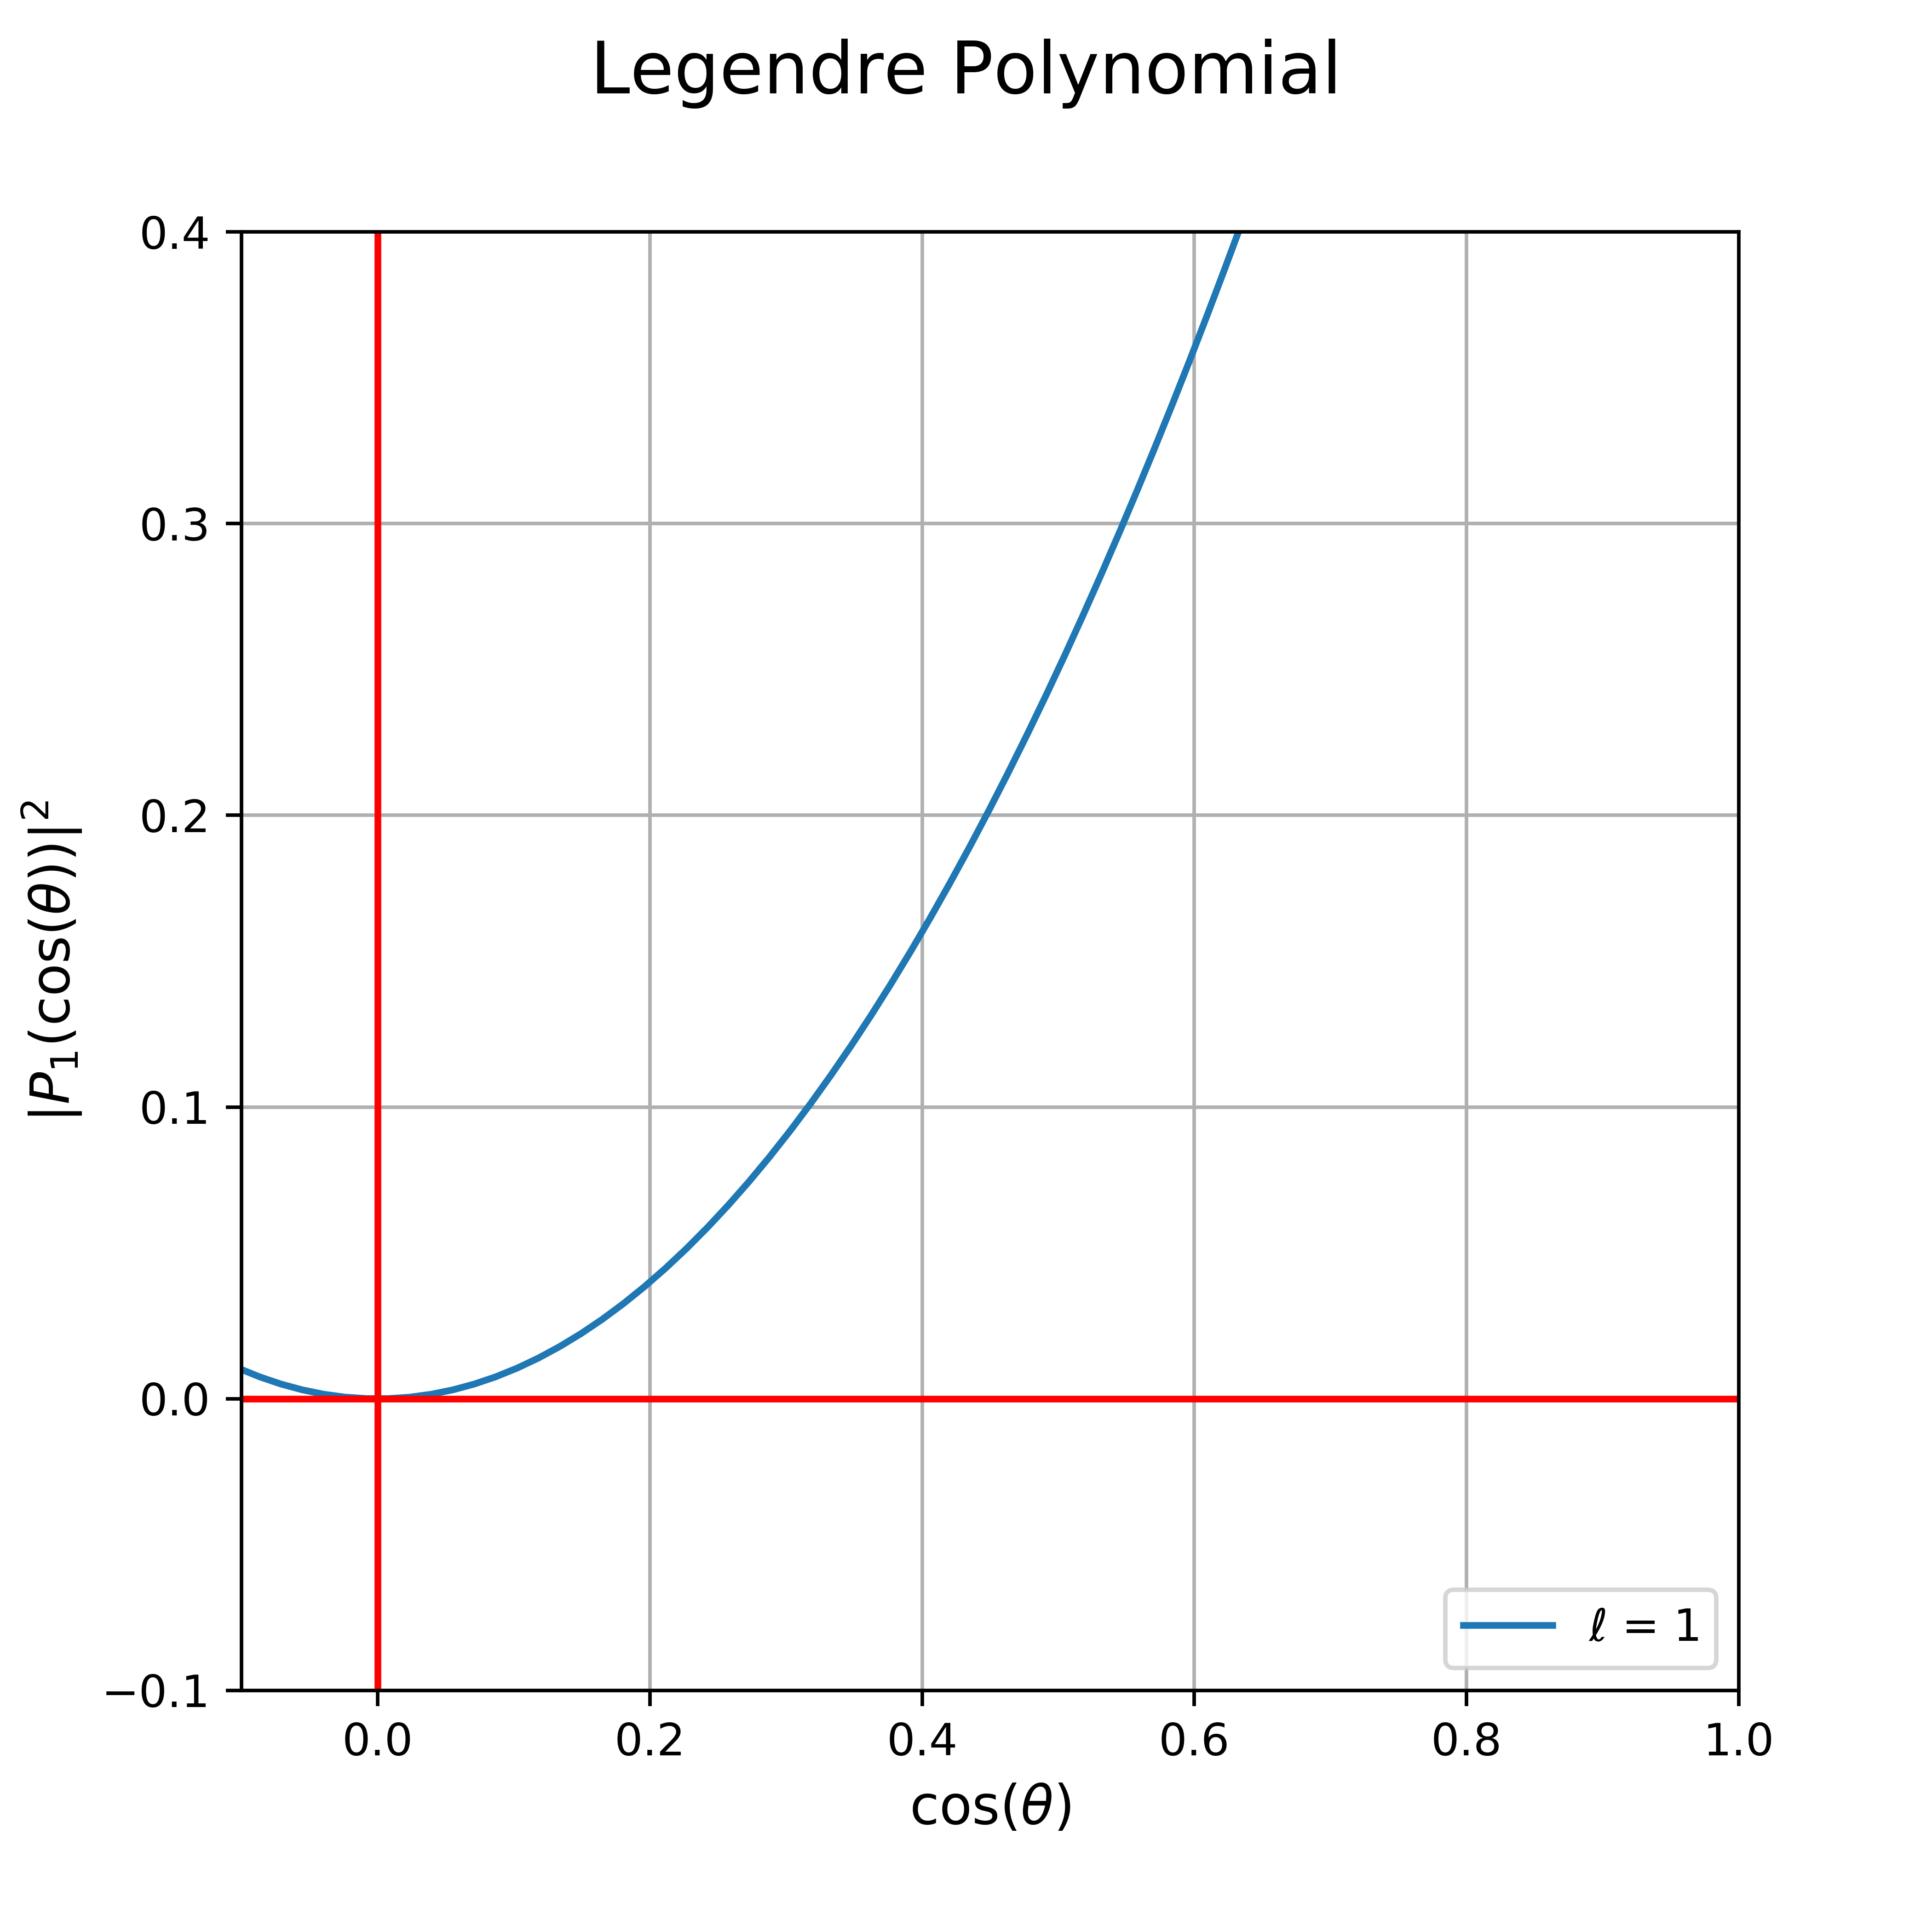
\includegraphics[height=6cm]{Legendre/legendreL1.png}\label{L1}}
	\caption{Comparison of the measured data and the $\ell=1$ Legendre polynomial for the $2291$ Hz resonance.}
	\label{legendre1}
\end{figure}

\begin{figure}[H]
	\centering
	\subfloat[Measured acoustic amplitude plotted against $\cos(\theta)$ for the 3679 Hz resonance]{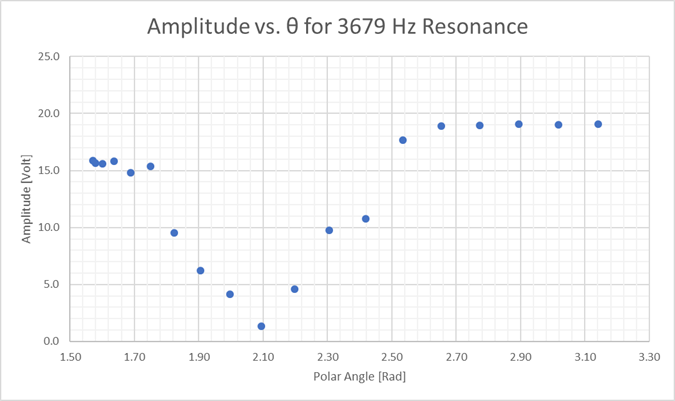
\includegraphics[height=6cm]{Graphs/3679Graph.png}}
	\qquad
	\subfloat[Legendre polynomial $|\mathrm{P}_2|^2$]{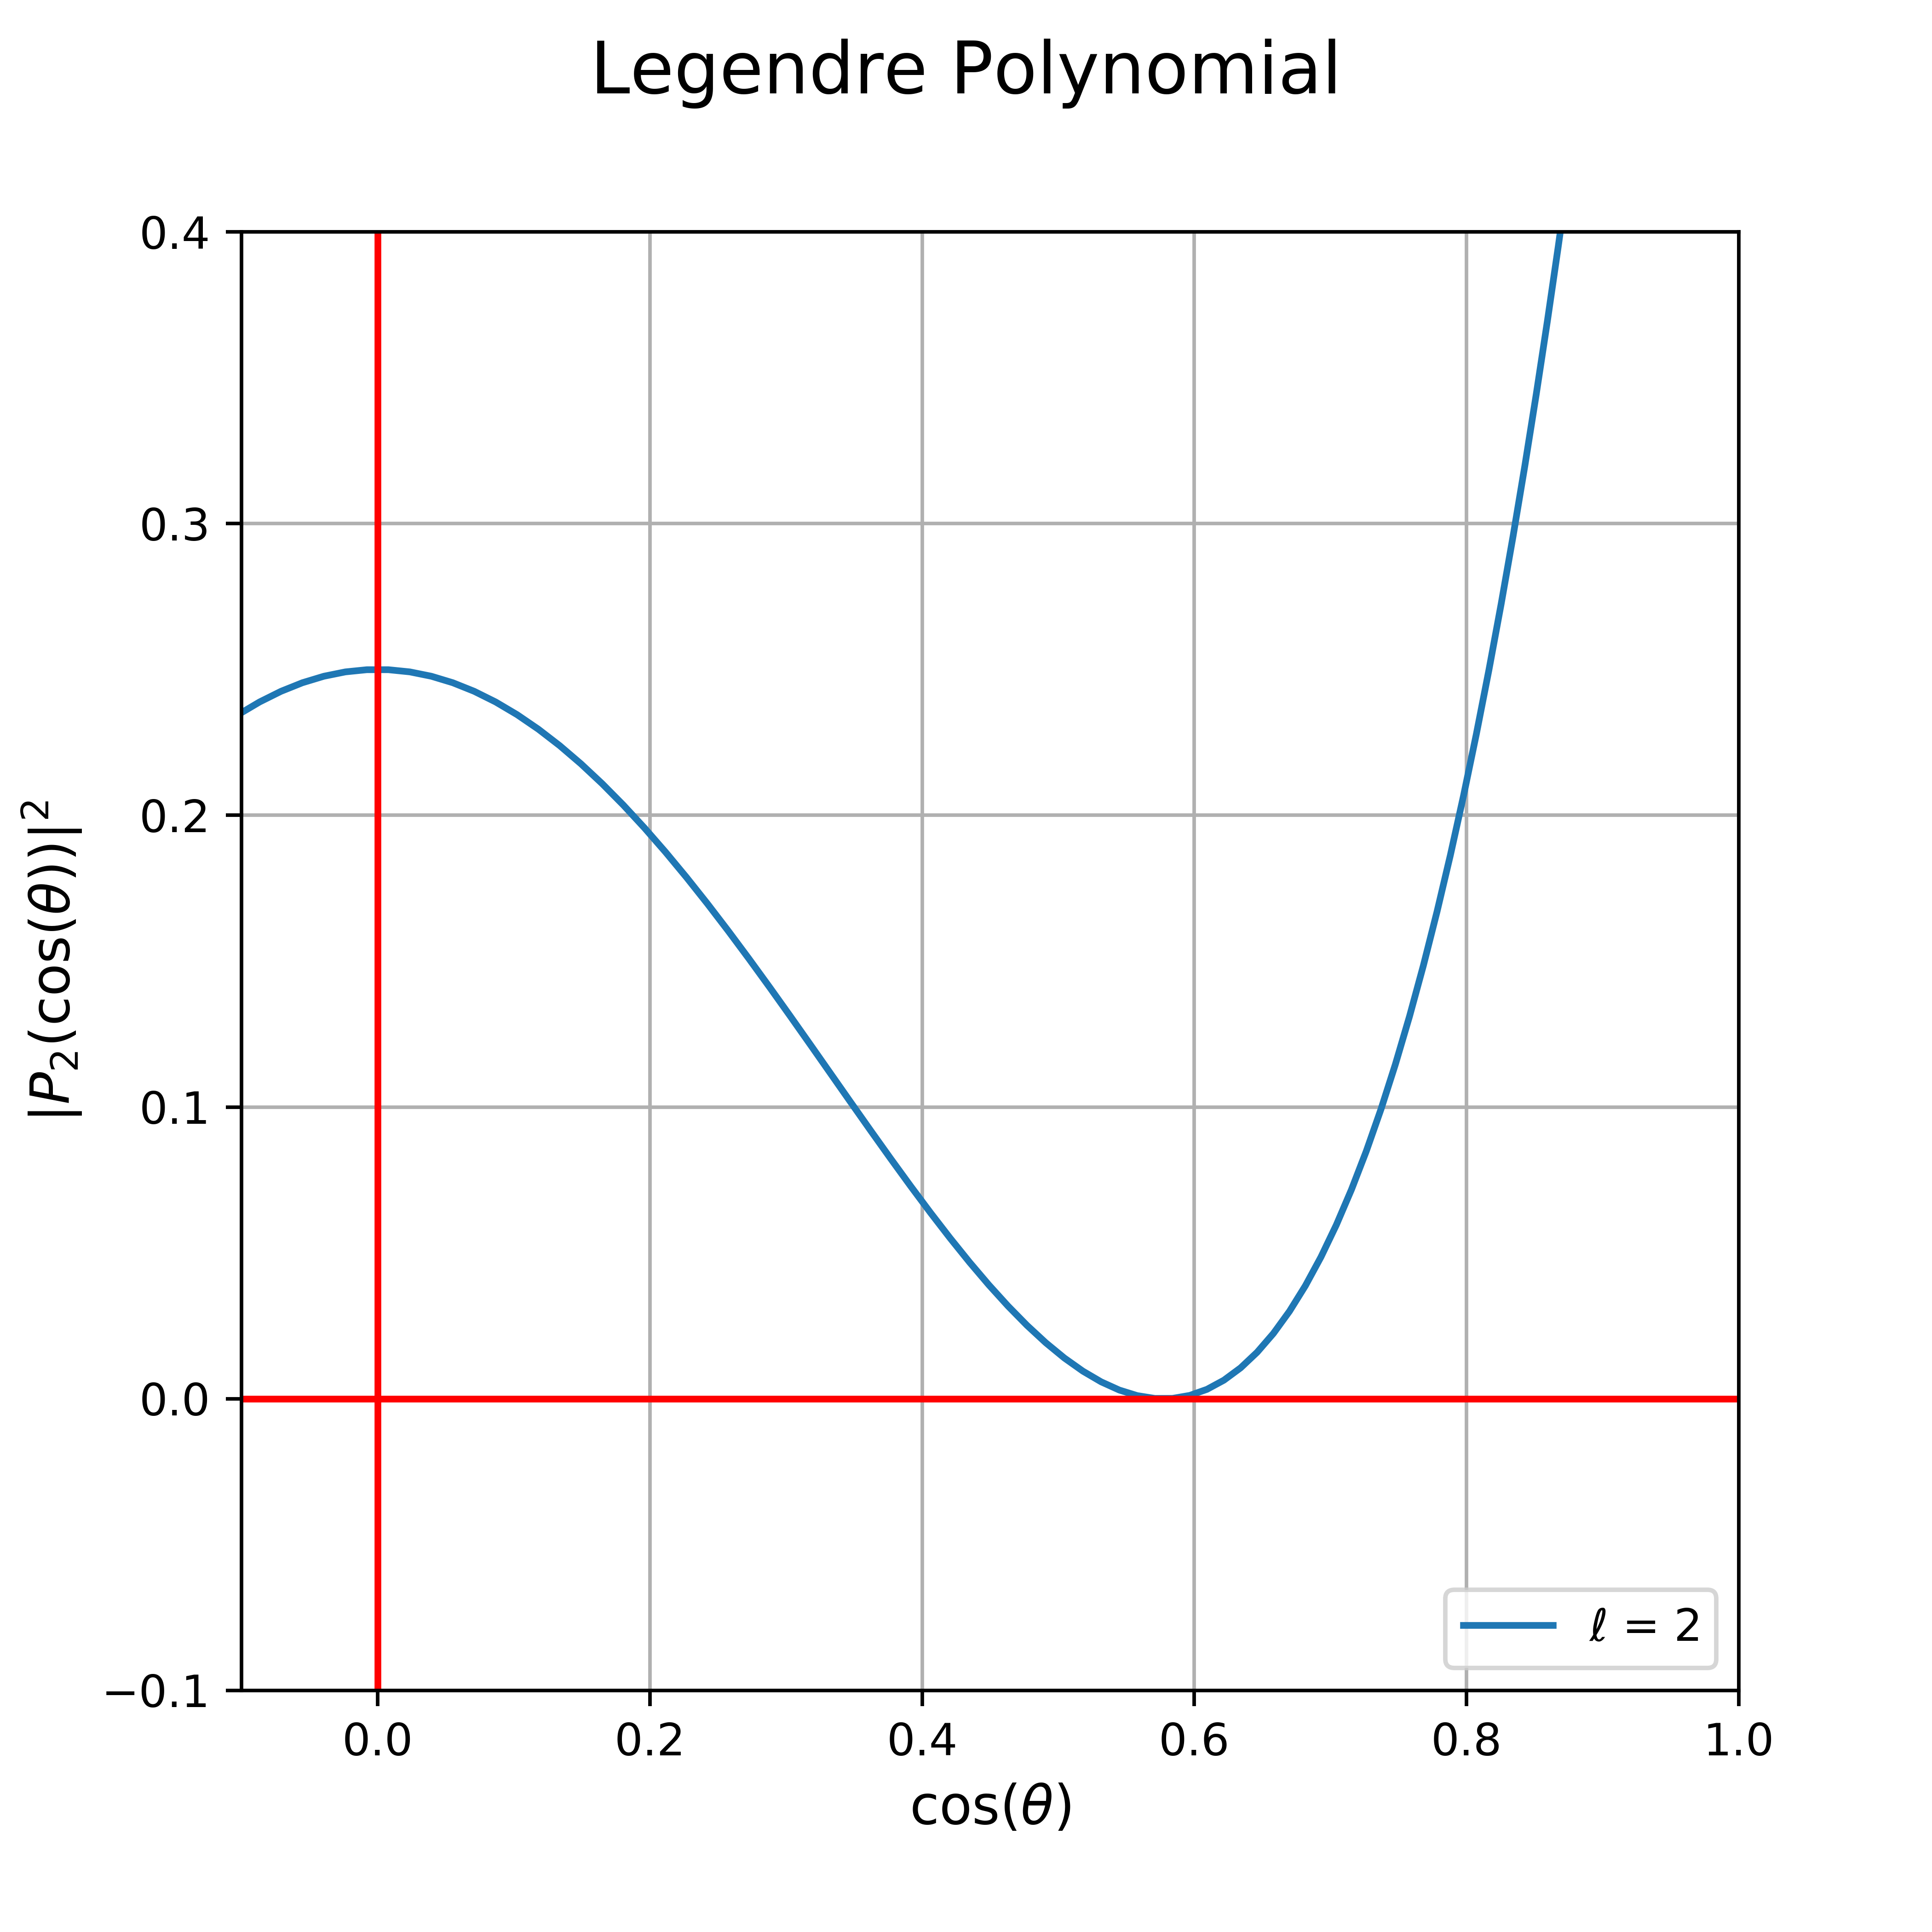
\includegraphics[height=6cm]{Legendre/legendreL2.png}\label{L2}}
	\caption{Comparison of the measured data and the $\ell=2$ Legendre polynomial for the $3679$ Hz resonance.}
	\label{legendre2}
\end{figure}

\begin{figure}[H]
	\centering
	\subfloat[Measured acoustic amplitude plotted against $\cos(\theta)$ for the 4962 Hz resonance]{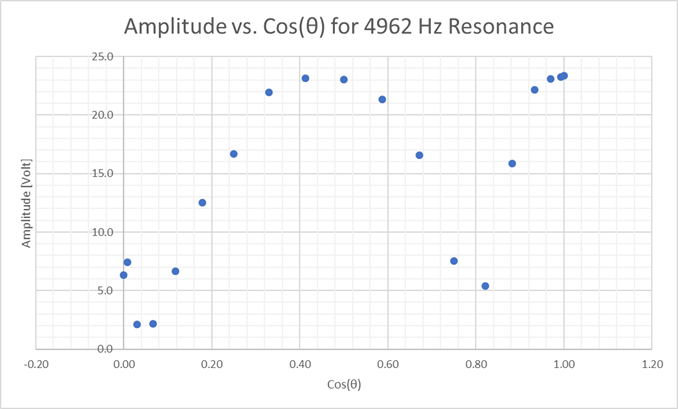
\includegraphics[height=6cm]{Graphs/4962Graph.png}}
	\qquad
	\subfloat[Legendre polynomial $|\mathrm{P}_3|^2$]{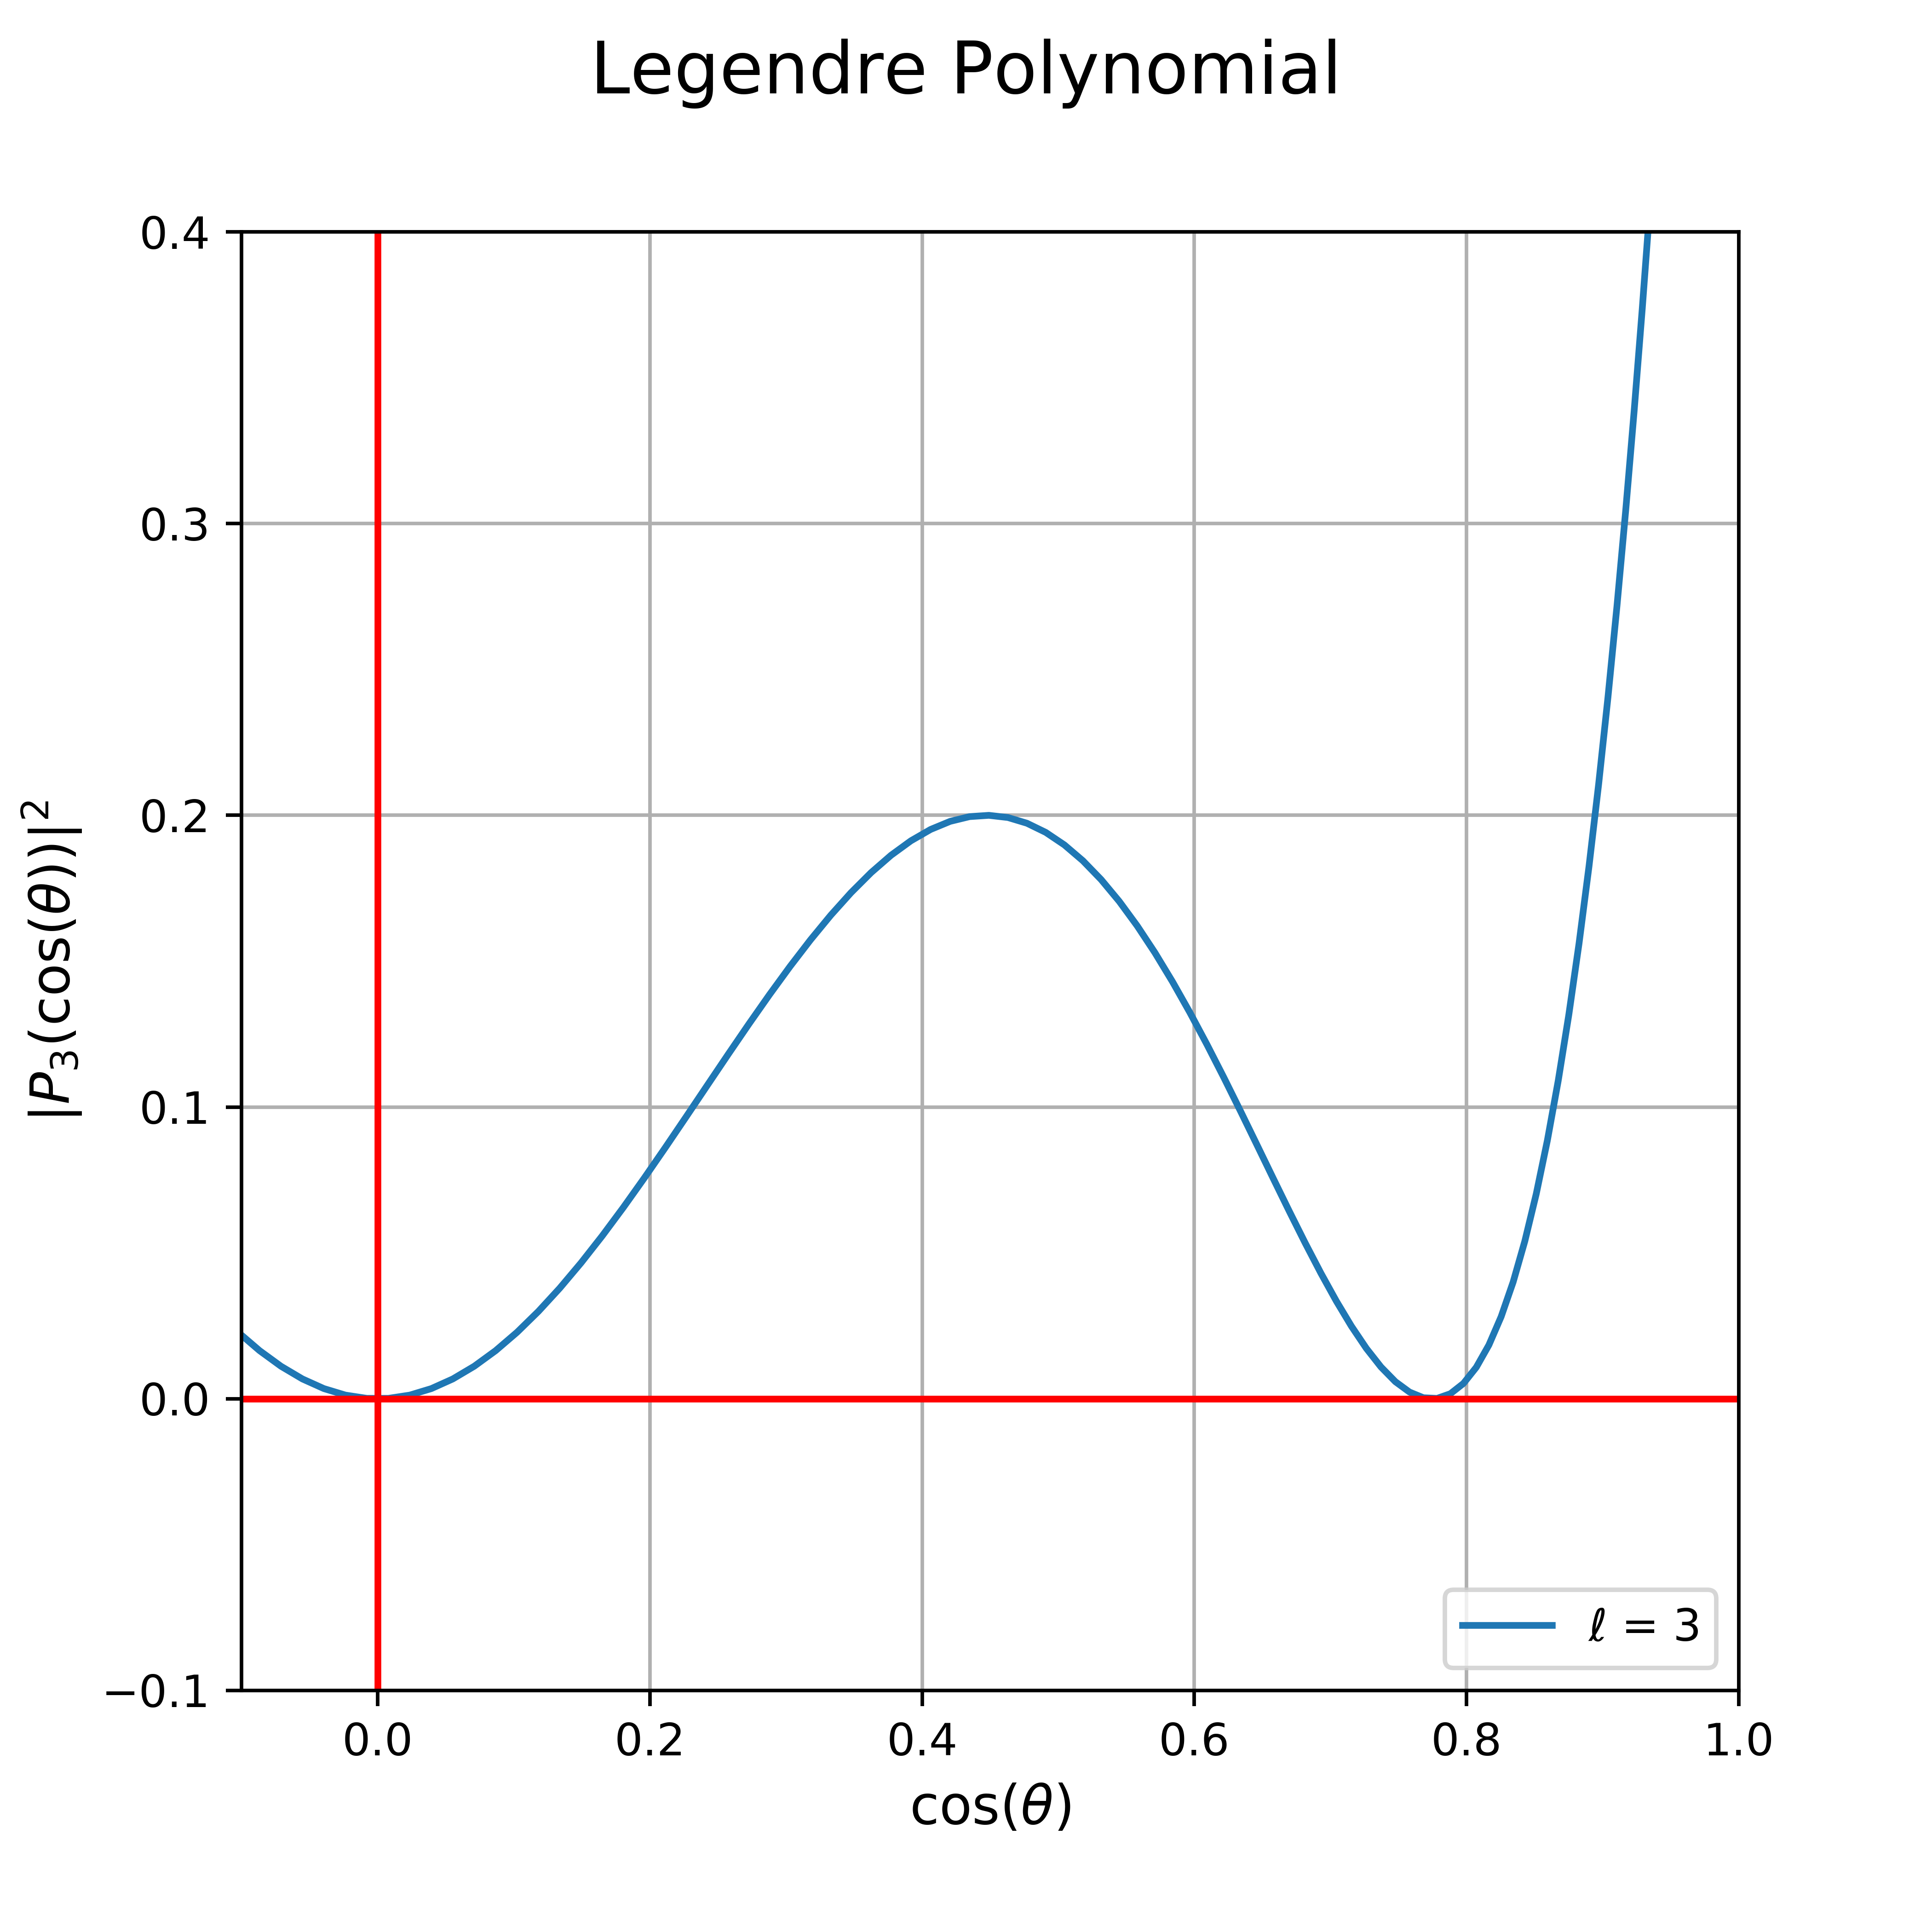
\includegraphics[height=6cm]{Legendre/legendreL3.png}\label{L3}}
	\caption{Comparison of the measured data and the $\ell=3$ Legendre polynomial for the $4962$ Hz resonance.}
	\label{legendre3}
\end{figure}

\begin{figure}[H]
	\centering
	\subfloat[Measured acoustic amplitude plotted against $\cos(\theta)$ for the 6202 Hz resonance]{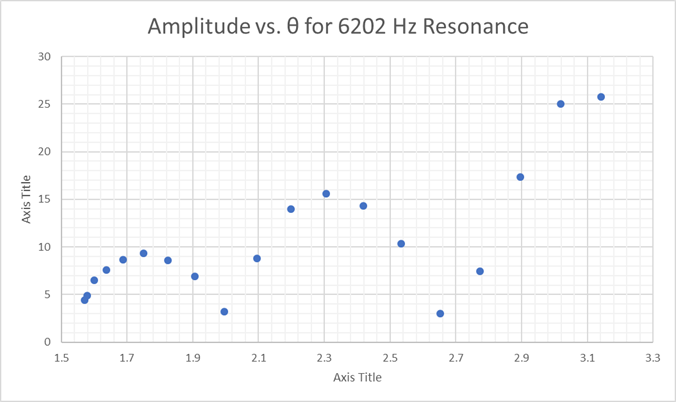
\includegraphics[height=6cm]{Graphs/6202Graph.png}}
	\qquad
	\subfloat[Legendre polynomial $|\mathrm{P}_4|^2$]{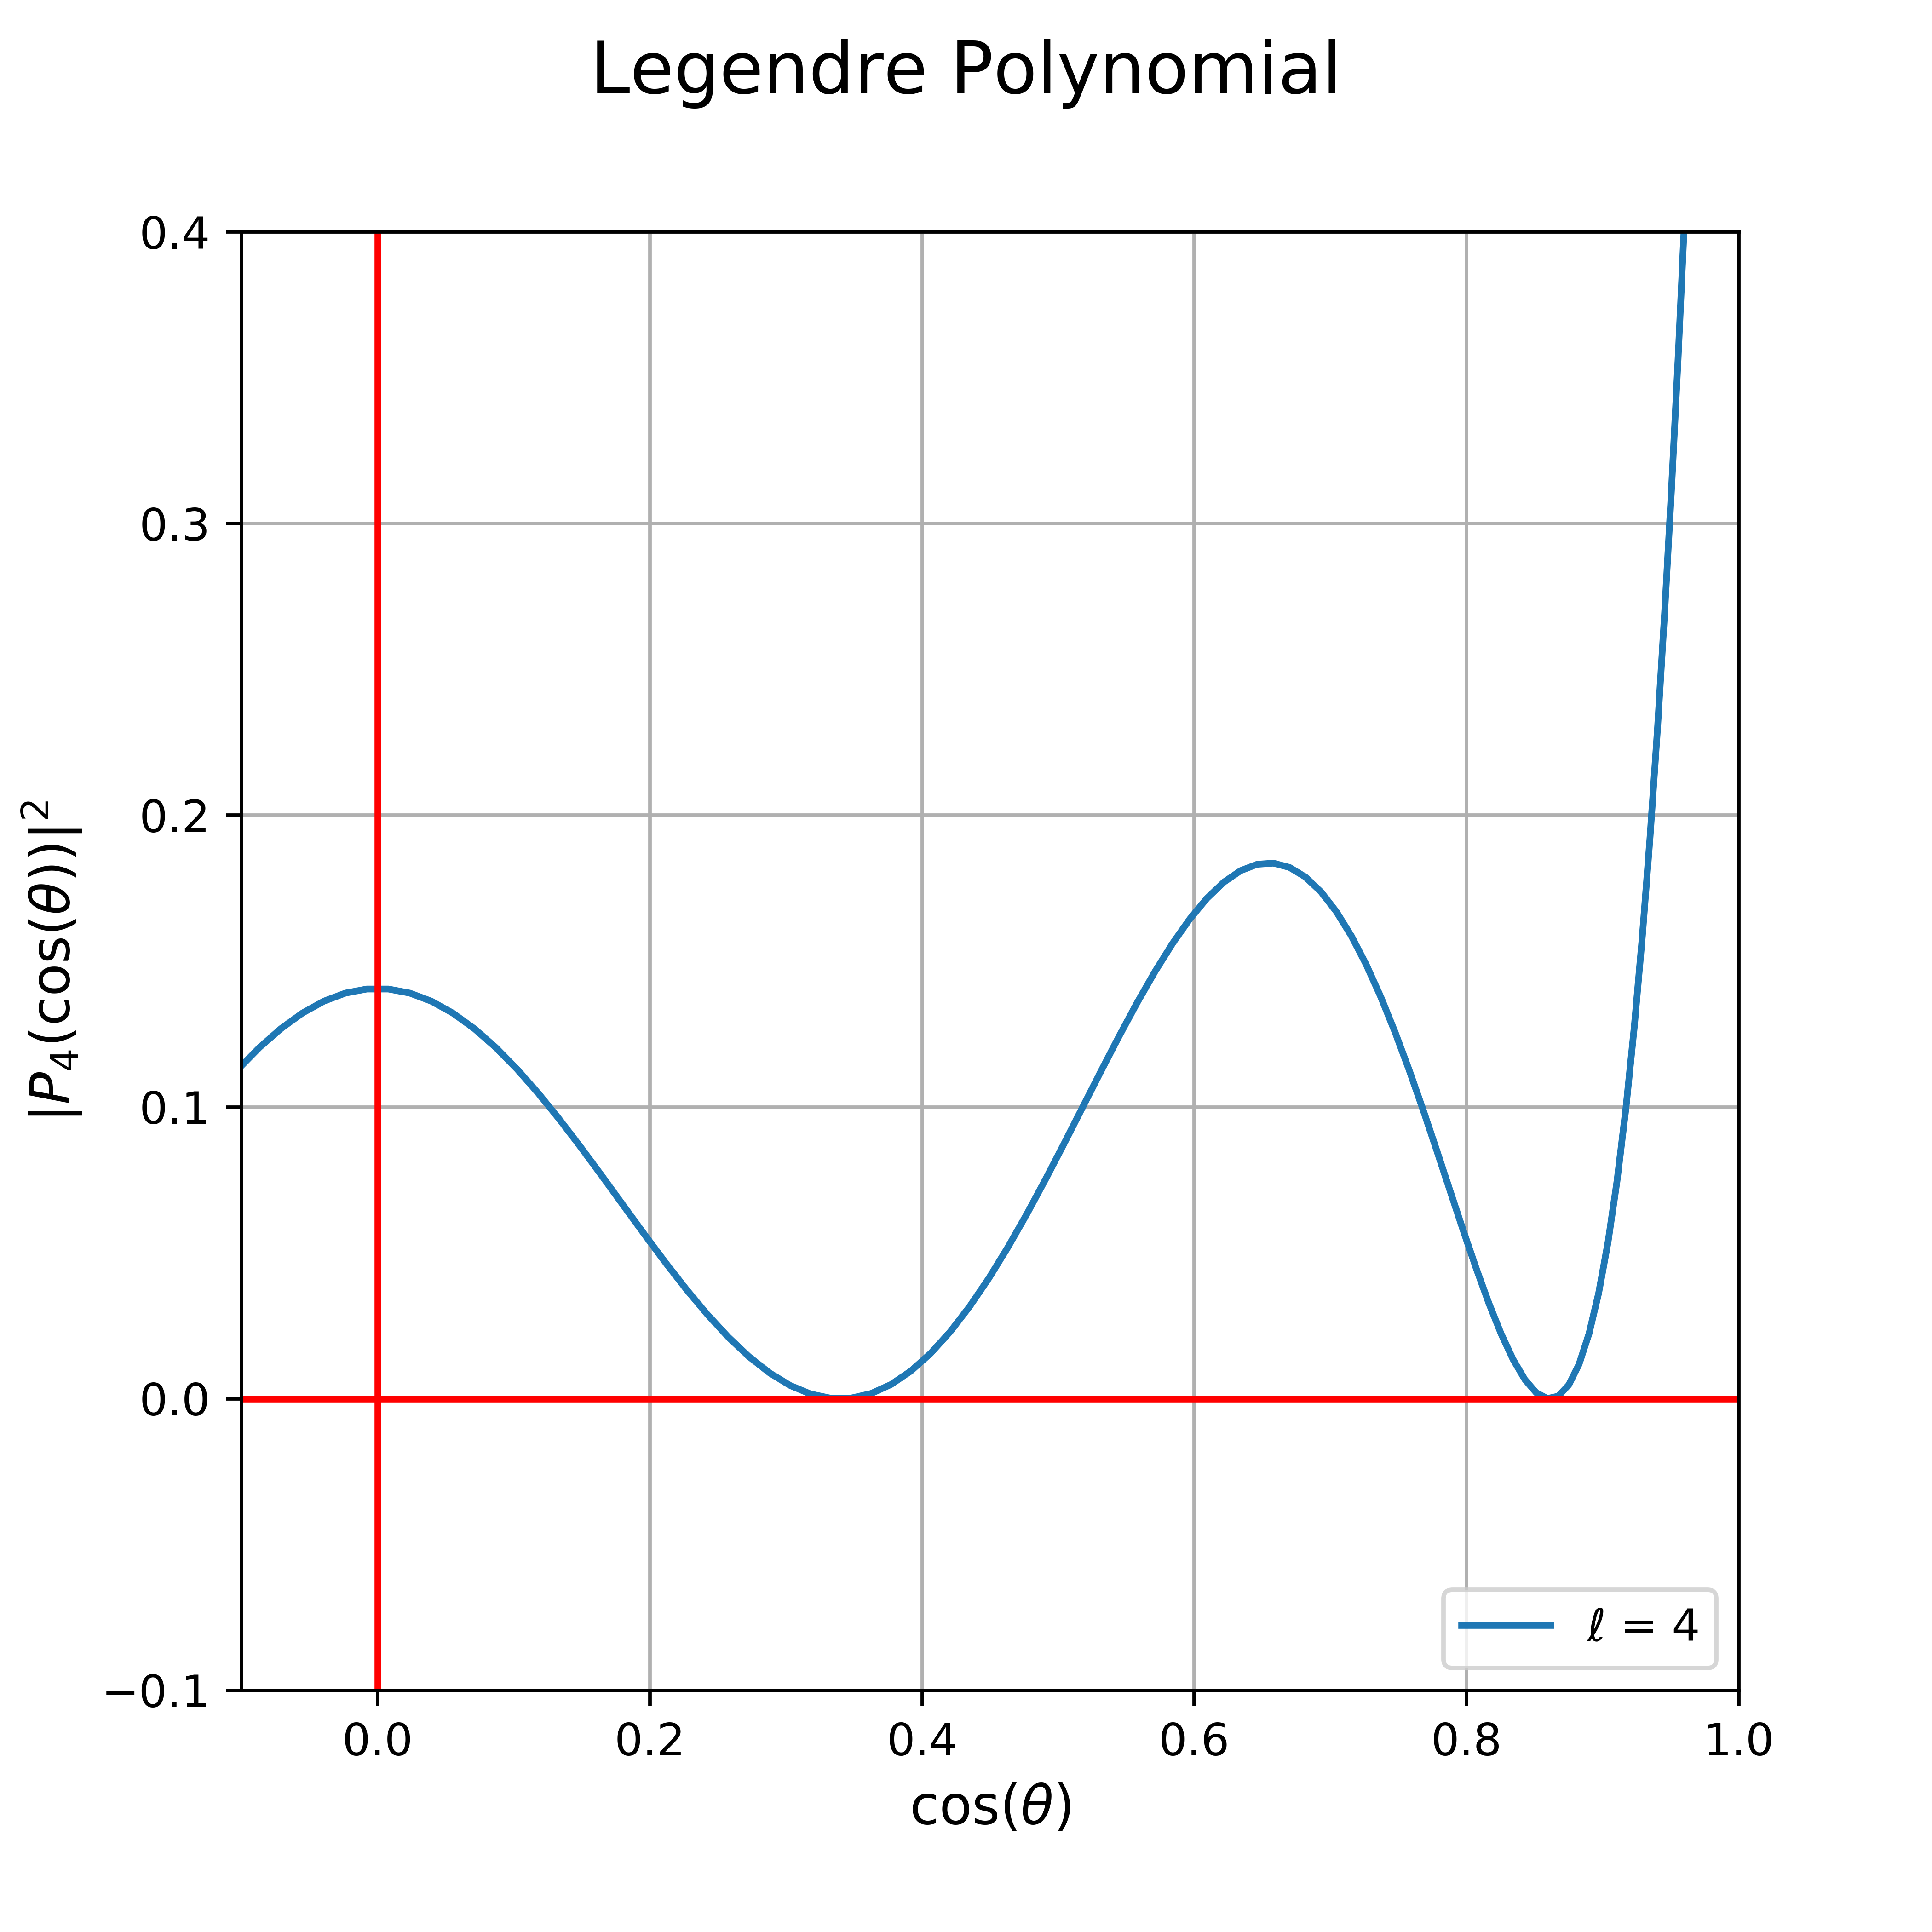
\includegraphics[height=6cm]{Legendre/legendreL4.png}\label{L4}}
	\caption{Comparison of the measured data and the $\ell=4$ Legendre polynomial for the $6202$ Hz resonance.}
	\label{legendre4}
\end{figure}

\begin{figure}[H]
	\centering
	\subfloat[Measured acoustic amplitude plotted against $\cos(\theta)$ for the 7409 Hz resonance]{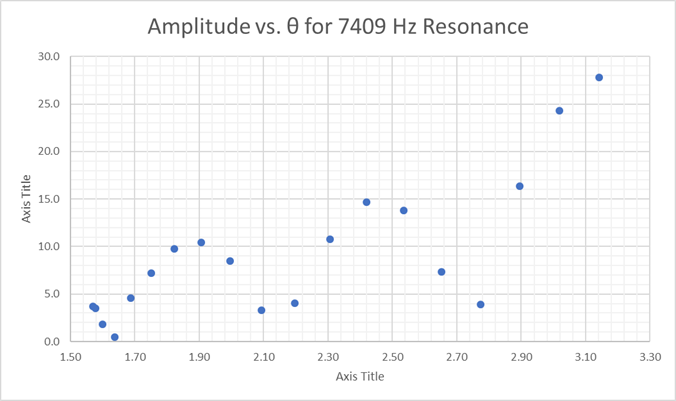
\includegraphics[height=6cm]{Graphs/7409Graph.png}}
	\qquad
	\subfloat[Legendre polynomial $|\mathrm{P}_5|^2$]{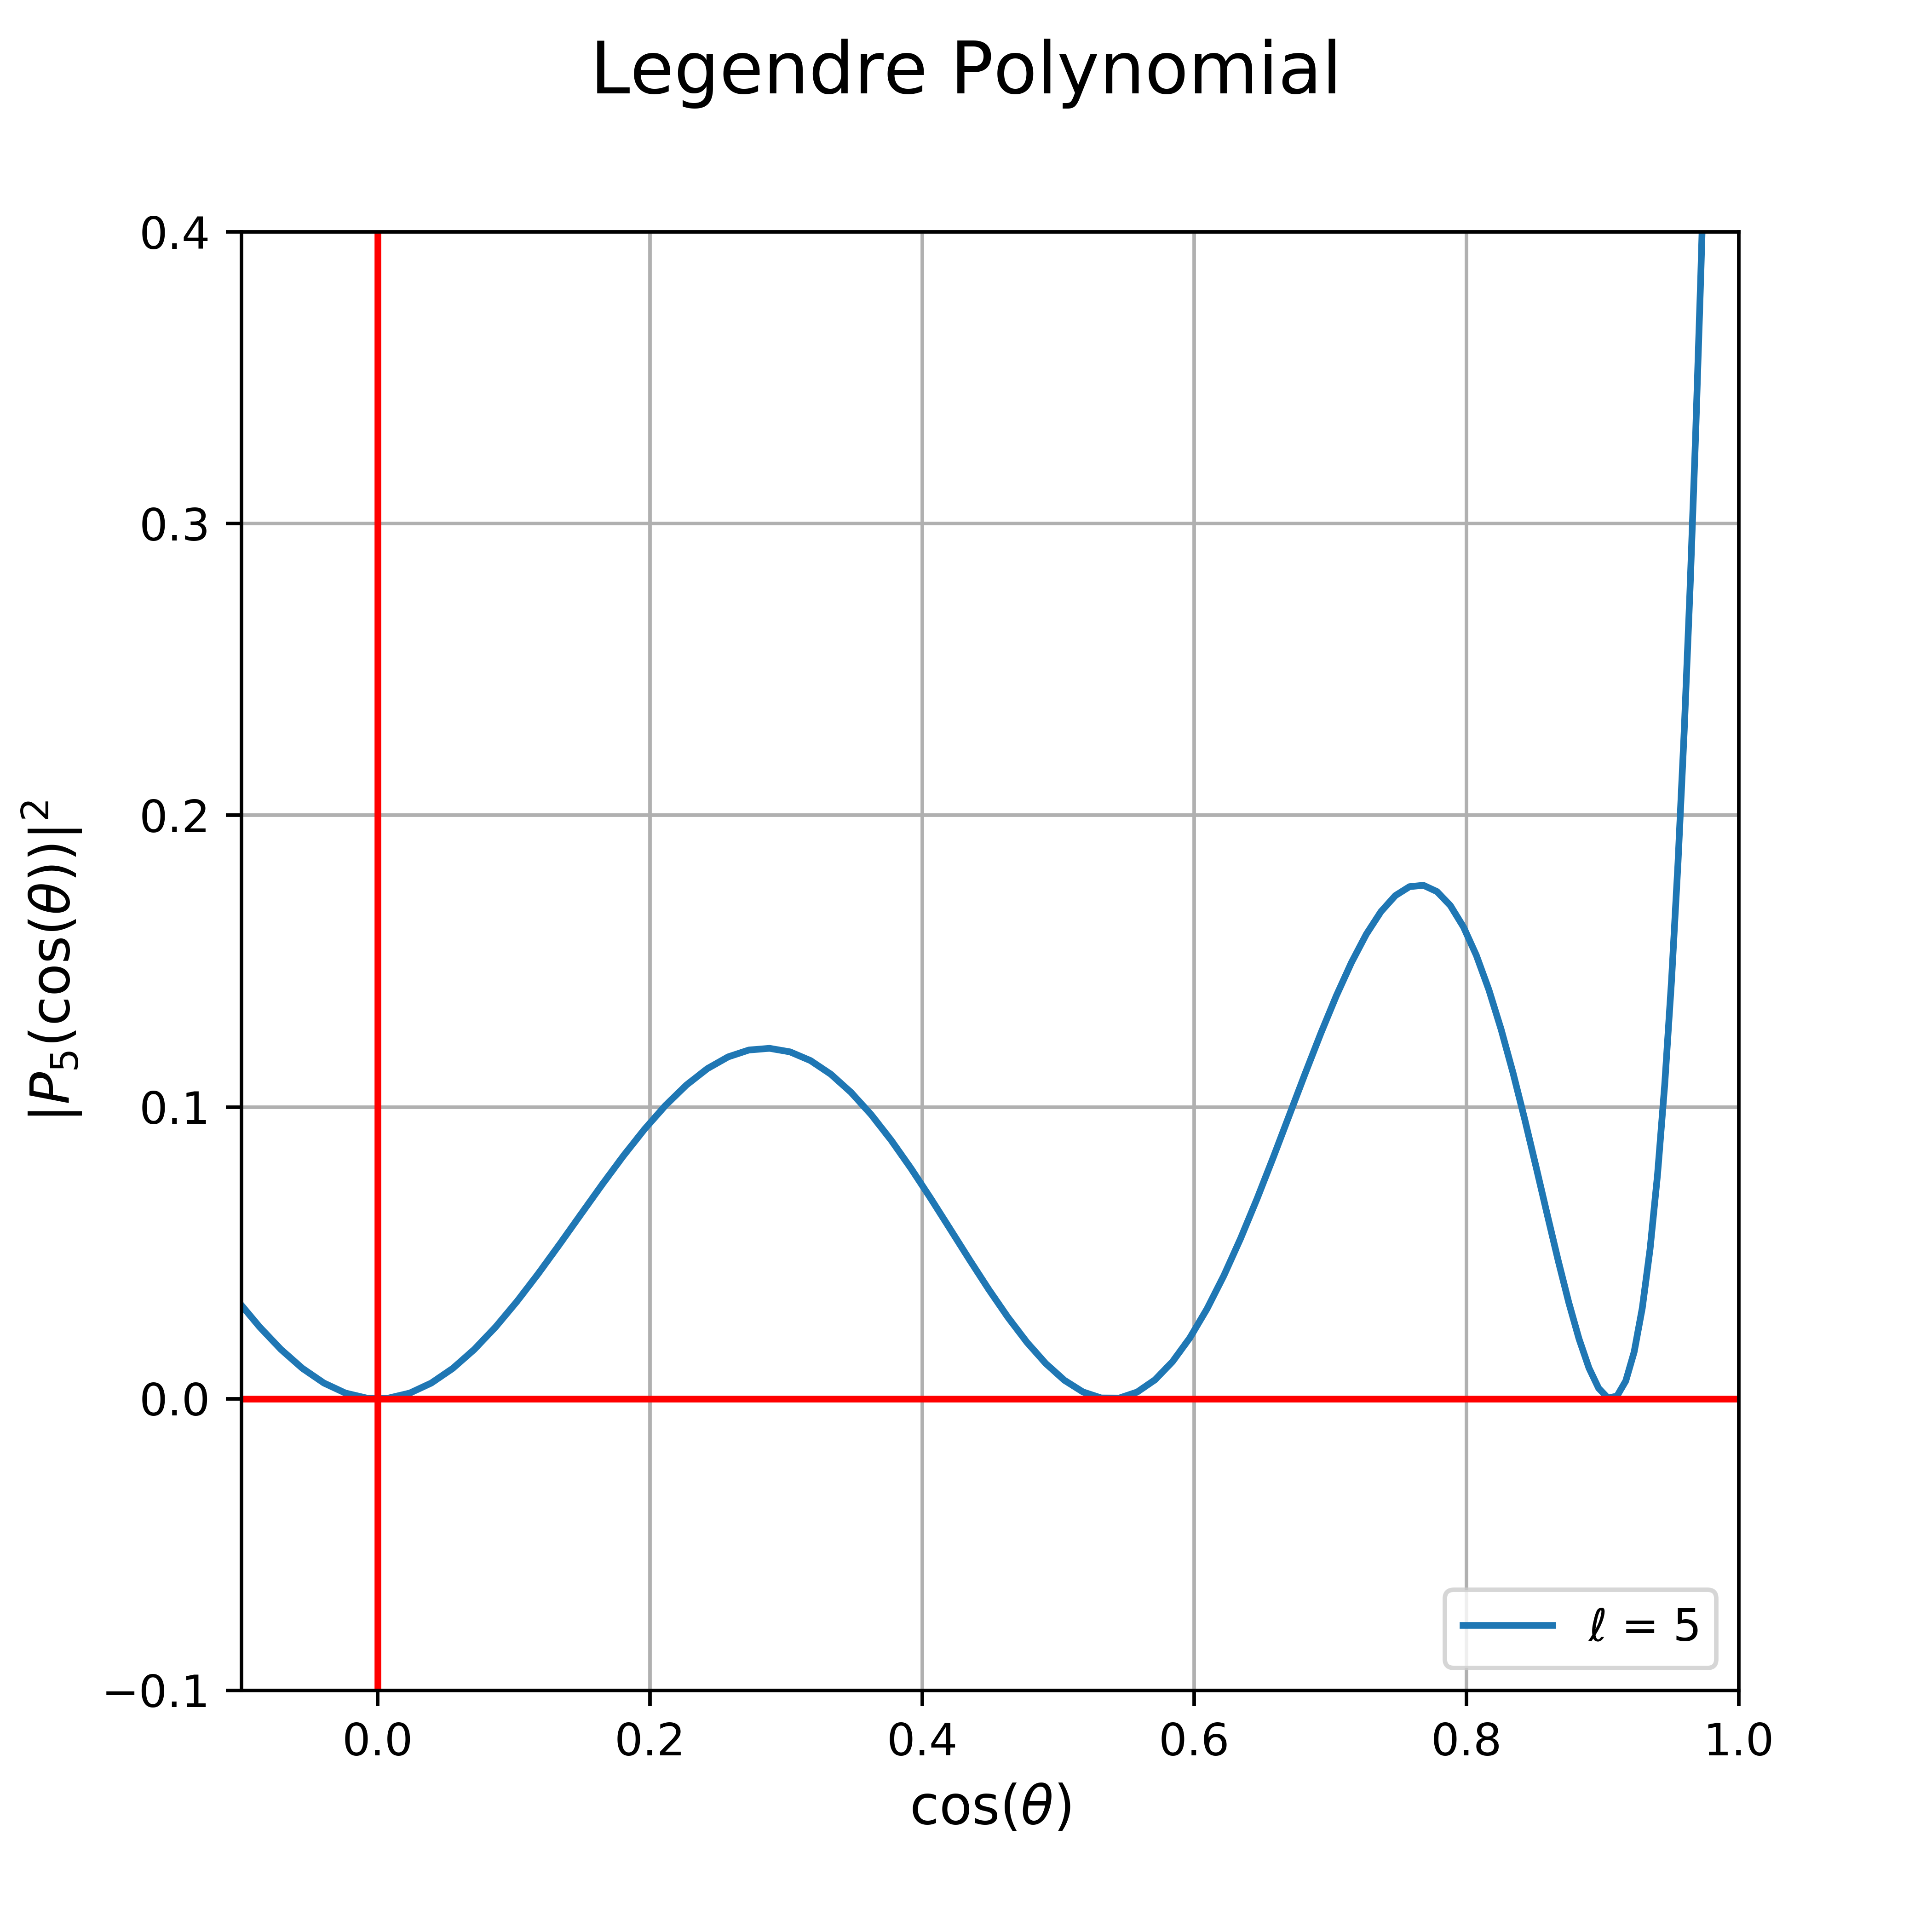
\includegraphics[height=6cm]{Legendre/legendreL5.png}\label{L5}}
	\caption{Comparison of the measured data and the $\ell=5$ Legendre polynomial for the $7409$ Hz resonance.}
	\label{legendre5}
\end{figure}

\subsection{Spherical Harmonics}


\begin{figure}[H]
	\centering
	\subfloat[$\ell=1$, $m=0$ polar plot for 2291 Hz resonance]{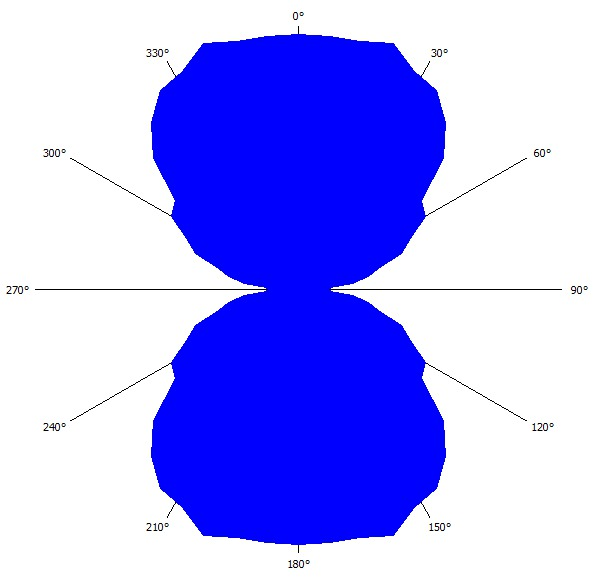
\includegraphics[width=0.35\textwidth]{2.3.2/F2291.jpg}\label{Polar2291}}
	\qquad \qquad
	\subfloat[$\ell=2$, $m=0$  plot for 3679 Hz resonance ]{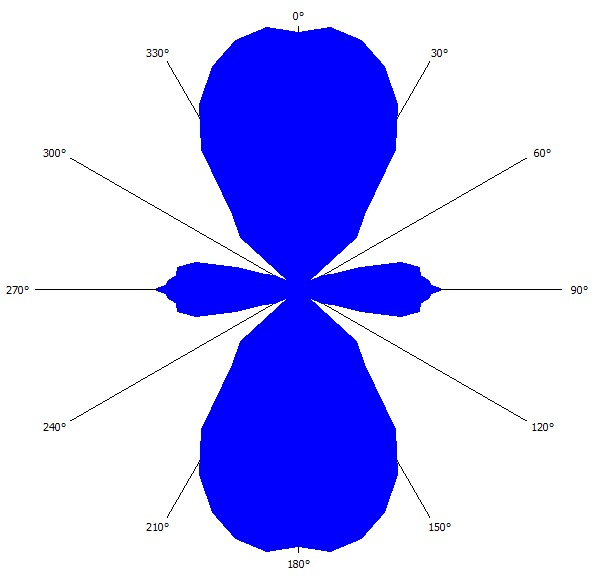
\includegraphics[width=0.35\textwidth]{2.3.2/F3679.jpg}\label{Polar3679}}
	\\
	\subfloat[$\ell=3$, $m=0$  plot for 4962 Hz resonance]{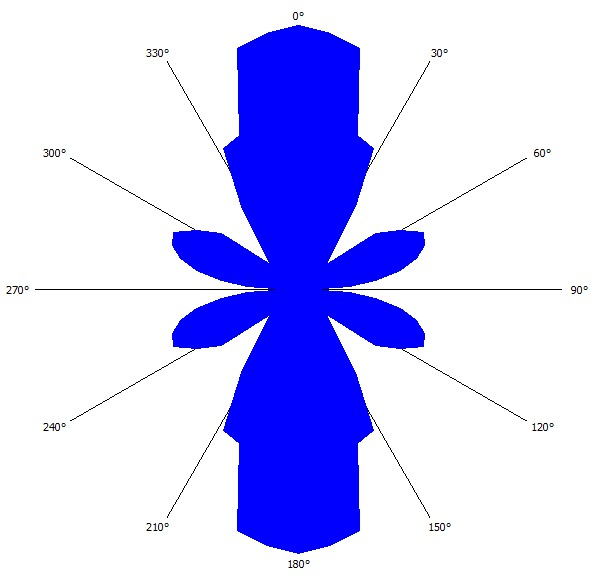
\includegraphics[width=0.35\textwidth]{2.3.2/F4962.jpg}\label{Polar4962}}
	\qquad \qquad
	\subfloat[$\ell=5$, $m=0$  plot for 7409 Hz resonance]{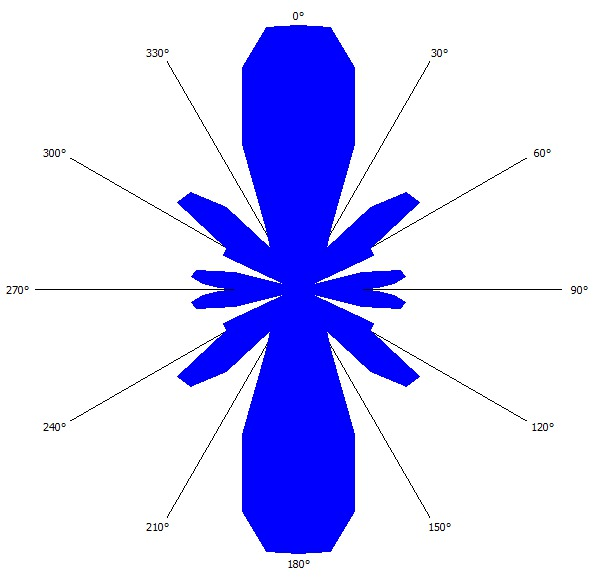
\includegraphics[width=0.35\textwidth]{2.3.2/F7409.jpg}\label{Polar6202}}
	\caption{Acoustic amplitude vs polar angle ($\theta$) with azimuthal angle $\varphi = 0$ for 4 resonant frequencies. Comparing these to the spherical harmonics in \cref{sphereHarm}, it is possible to determine the angular momentum quantum number $\ell$ for each resonance.}
	\label{polarGraphs}
\end{figure}

\begin{figure}[H]
	\centering
	\subfloat[Spherical harmonic for $\ell = 1$, $m= 0$]{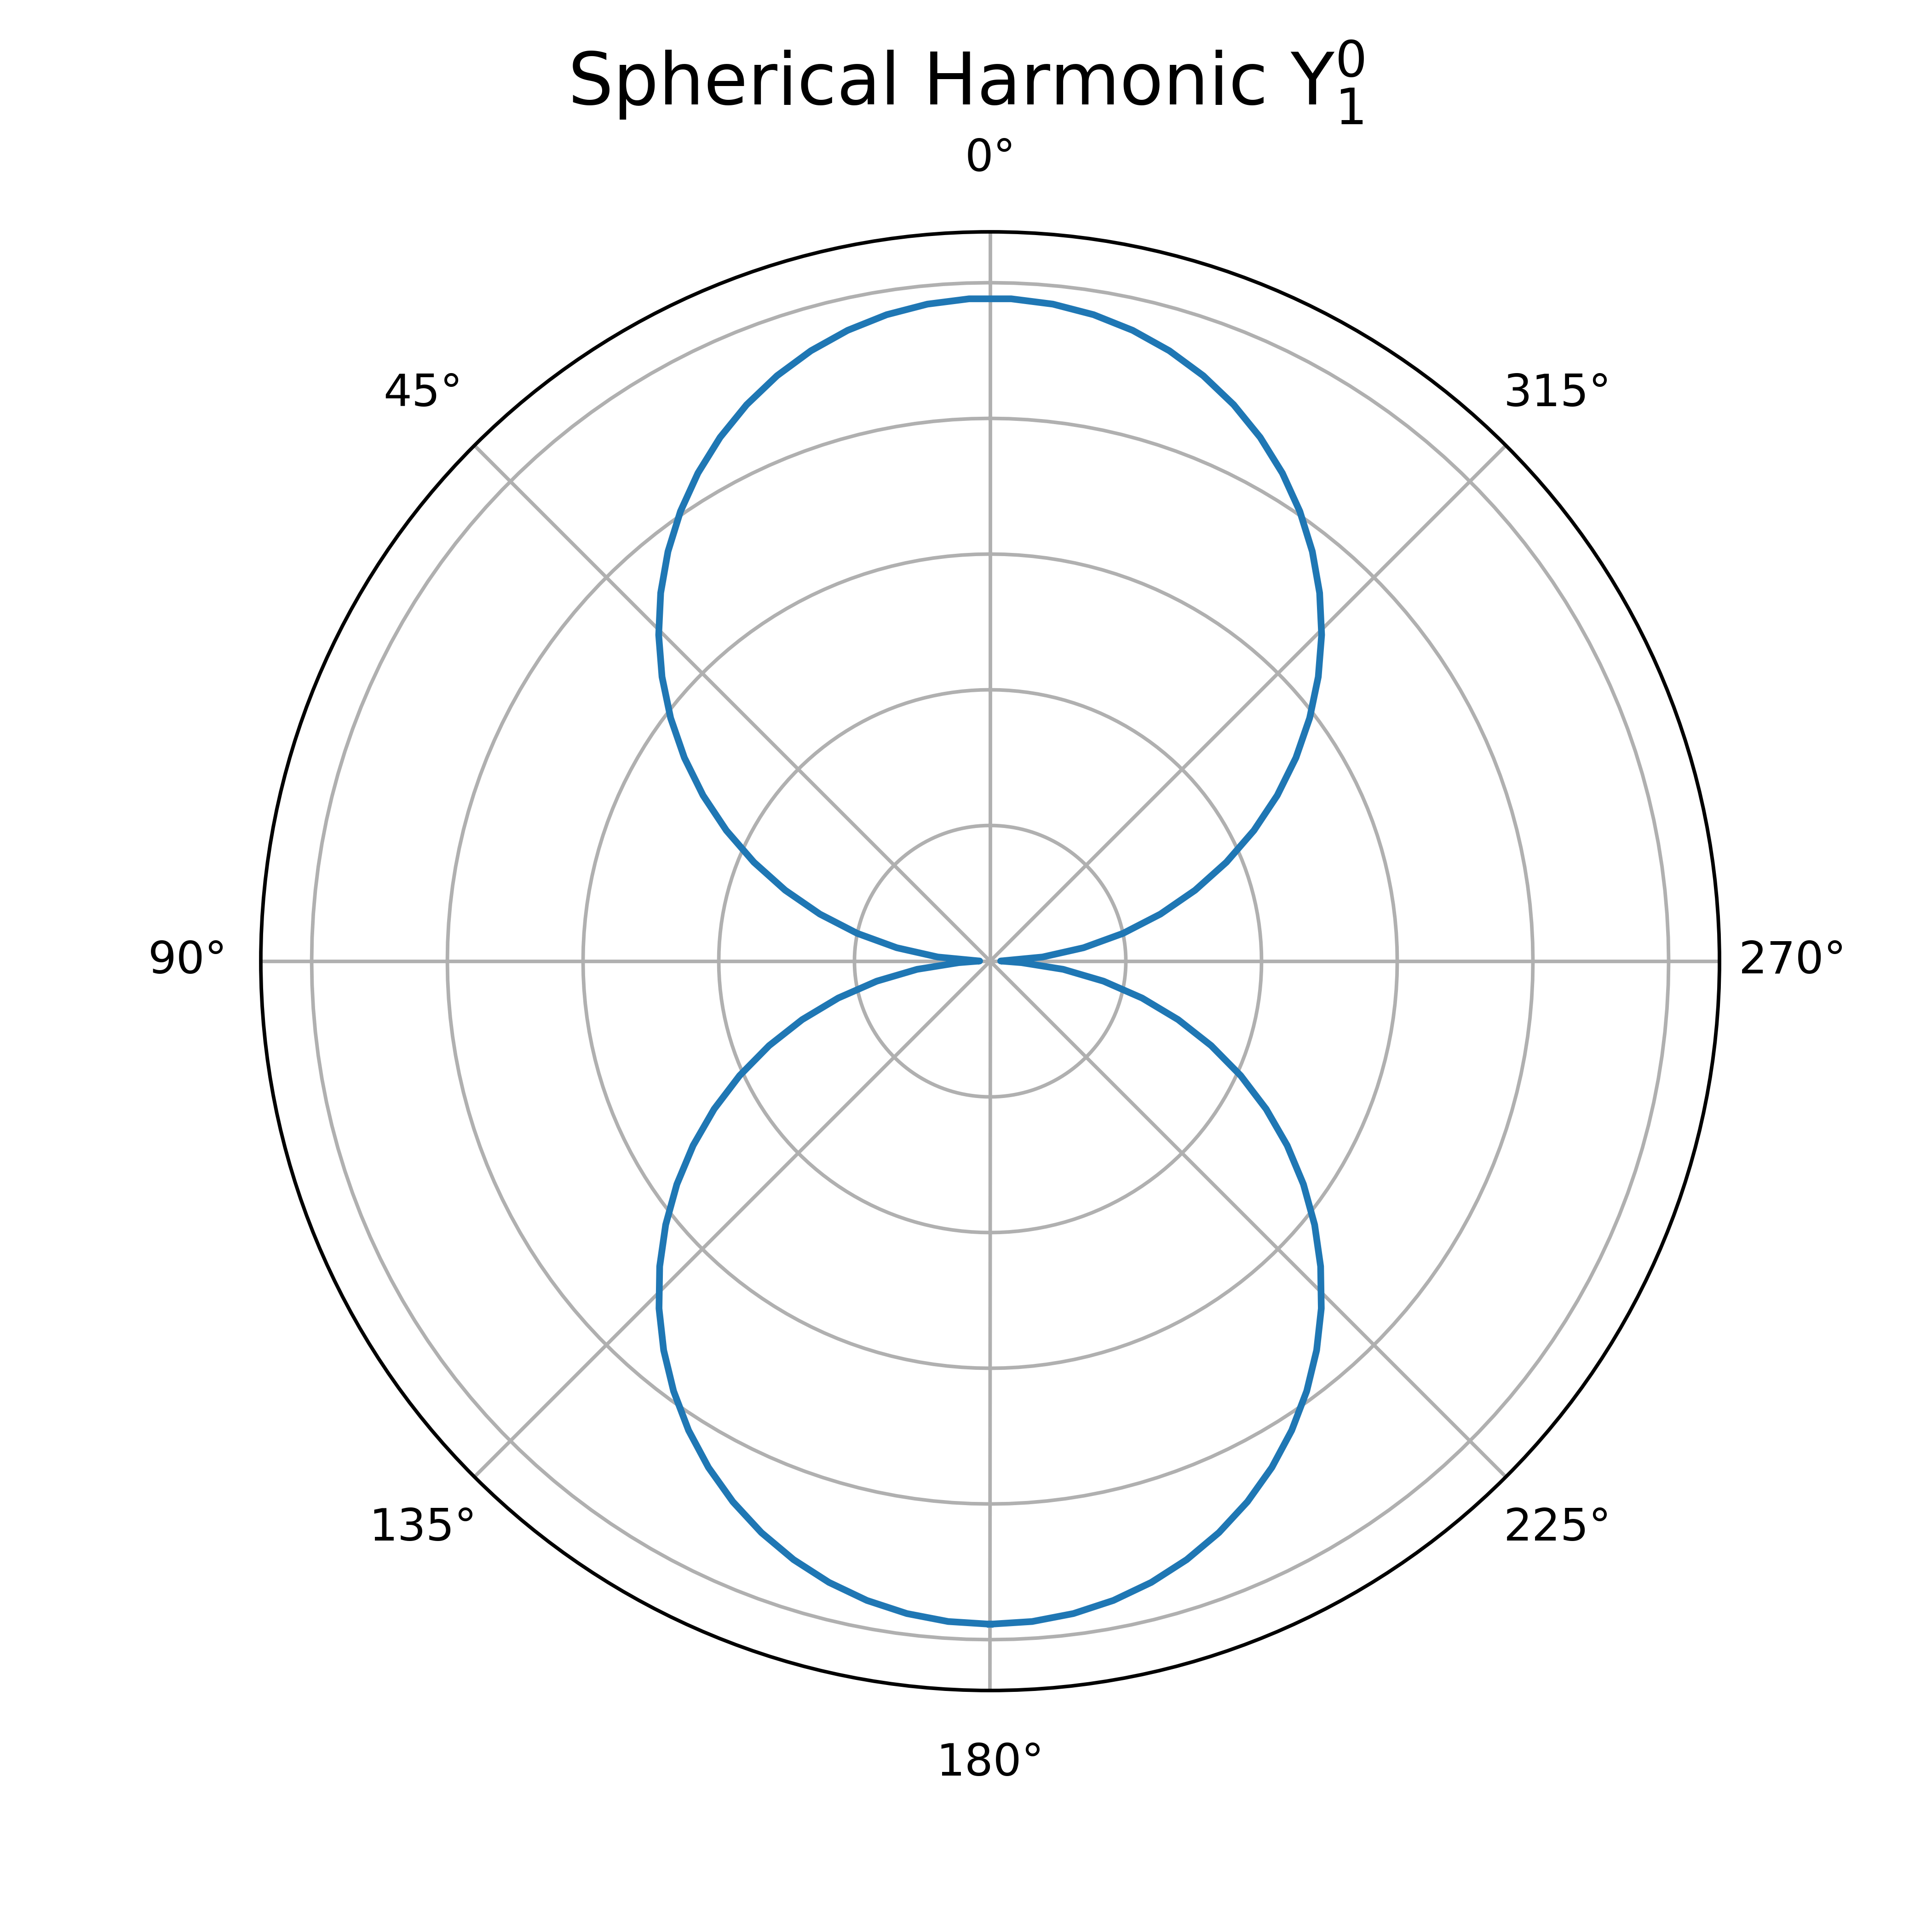
\includegraphics[width=0.4\textwidth]{SphHarm/SphHarmL1M0.png}\label{sphHarmL1M0}}
	\qquad \quad
	\subfloat[Spherical harmonic for $\ell = 2$, $m=0$]{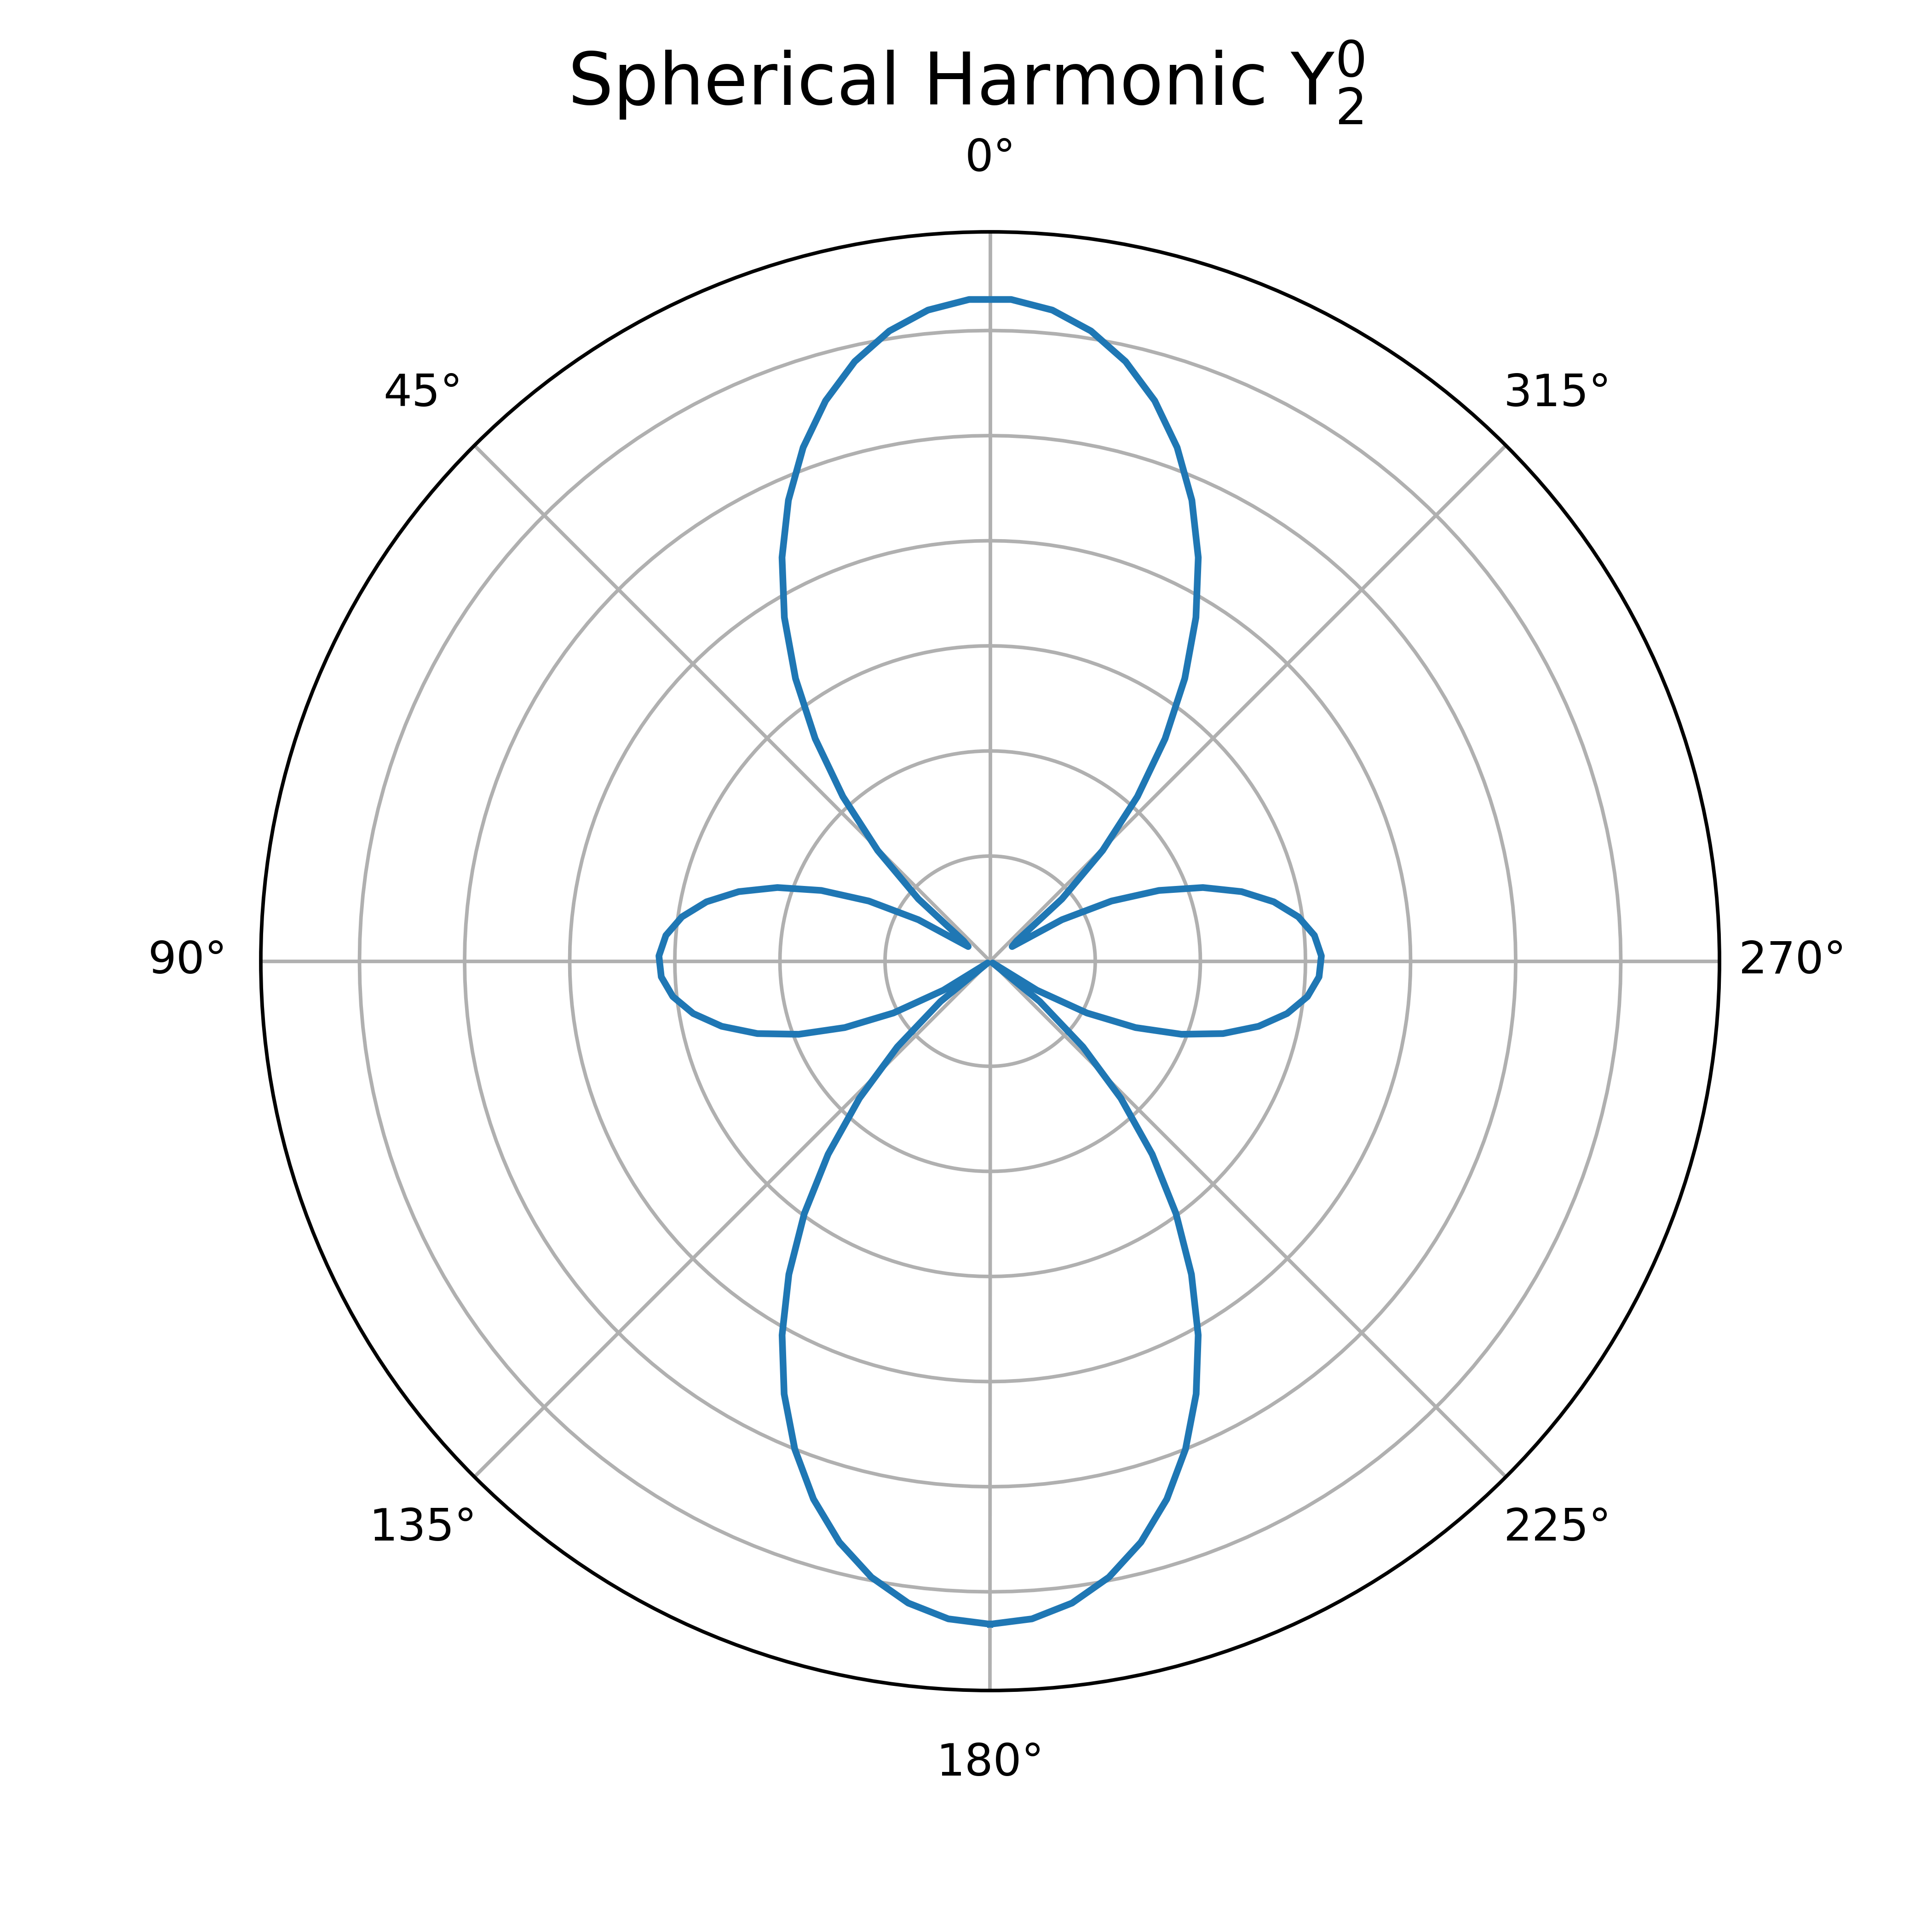
\includegraphics[width=0.4\textwidth]{SphHarm/SphHarmL2M0.png}\label{sphHarmL2M0}}
	\\
	\subfloat[Spherical harmonic for $\ell = 3$, $m = 0$]{\includegraphics[width=0.4\textwidth]{SphHarm/SphHarmL3M0.png}\label{sphHarmL3M0}}
	\qquad \quad
	\subfloat[Spherical harmonic for $\ell = 5$, $m = 1$]{\includegraphics[width=0.4\textwidth]{SphHarm/SphHarmL5M0.png}\label{sphHarmL5M0}}
	\caption{Projections of the spherical harmonics $\mathrm{Y}^\ell_m$ onto the $\varphi = 0$ plane. Angle markings indicate polar angle $\theta$.}
	\label{sphereHarm}
\end{figure}

\subsection{Polar Graphs with Broken Cavity Symmetry}


\begin{figure}[H]
	\captionsetup{justification = centering}
	\centering
	\subfloat[$\ell=1$, $m=0$]{\includegraphics[width=0.35\textwidth]{Day4/L13mmPolar2084_806.png}}
	\qquad \quad
	\subfloat[$\ell=1$, $m=\pm1$]{\includegraphics[width=0.35\textwidth]{Day4/L13mmPolar2251_140.png}}
	\caption{Amplitude versus polar angle $\theta$ for the $\ell=1$ resonance with 3mm Spacing}
	\label{3mmliftedDegeneracy}
\end{figure}


\begin{figure}[H]
	\captionsetup{justification = centering}
	\centering
	\subfloat[[$\ell=1$, $m=0$]{\includegraphics[width=0.35\textwidth]{Day4/L16mmPolar2084_806.png}}
	\qquad \quad
	\subfloat[[$\ell=1$, $m=\pm1$]{\includegraphics[width=0.35\textwidth]{Day4/L16mmPolar2251_140.png}}
	\caption{Amplitude versus polar angle $\theta$ for the $\ell=1$ resonance with 6mm Spacing}
	\label{6mmliftedDegeneracy}
\end{figure}

We can see that as the cavity separation is increased, simulating a stronger magnetic field, the shapes of the orbitals becomes more symmetric.


%	\begin{figure}[H]
%		\centering
%		\subfloat[$\ell=2$, $m=-1$ resonance]{\includegraphics[width=0.3\textwidth]{2.3.3/3mmPolar/323_Polar_L1M-1Amp_freq3591_549.png} \label{3-0mmDegeneracy}}
%		\quad
%		\subfloat[$\ell=2$, $m=0$ resonance]{\includegraphics[width=0.3\textwidth]{2.3.3/3mmPolar/323_Polar_L1M1Amp_freq3647_513.png} \label{3-1mmDegeneracy}}
%		\caption{Polar plots of lifted degeneracies for 3mm spacing}
%		\label{3mmliftedDegeneracy}
%	\end{figure}
%	It is important to note that not all the degeneracies were lifted at $3$ mm spacing.


%
%	\begin{figure}[H]
%		\centering
%		\subfloat[$\ell=1$, $m=-1$ resonance]{\includegraphics[width=0.3\textwidth]{2.3.3/6mmPolar/323_Polar_L1M-1Amp_freq3519_864.png} \label{6-m1mmDegeneracy}}
%		\quad
%		\subfloat[$\ell=1$, $m=0$ resonance]{\includegraphics[width=0.3\textwidth]{2.3.3/6mmPolar/323_Polar_L1M0Amp_freq3534_956.png} \label{6-0mmDegeneracy}}
%		\quad
%		\subfloat[$\ell=1$, $m=1$ resonance]{\includegraphics[width=0.3\textwidth]{2.3.3/6mmPolar/323_Polar_L1M1Amp_freq3632_422.png} \label{6-1mmDegeneracy}}
%		\caption{Polar plots of lifted degeneracies for 6mm spacing.}
%		\label{6mmliftedDegeneracy}
%	\end{figure}
%	
%	
%		Further, we focus on the \red{$\ell=2$} resonance and apply the spacing rings again to see how the peak splits.
%	
%	\begin{figure}[H]
%		\centering
%		\subfloat[Lifted degeneracy spectrum for $\ell=2$ 3mm spacing]{\includegraphics[width=0.3\textwidth]{2.3.3/323a180L13mmHires.png} \label{3mmDegeneracySpectrum}}
%		\quad
%		\subfloat[Lifted degeneracy spectrum for $\ell=2$ 6mm spacing]{\includegraphics[width=0.3\textwidth]{2.3.3/323a180L16mmHires.png} \label{6mmDegeneracySpectrum}}
%		\quad
%		\subfloat[Lifted degeneracy spectrum for $\ell=2$ 9mm spacing]{\includegraphics[width=0.3\textwidth]{2.3.3/323a180L19mmHires.png} \label{9mmDegeneracySpectrum}}
%		\caption{Progression of lifted degeneracies for the \red{$\ell=2$} state.}
%		\label{liftedDegeneracySpectrum}
%	\end{figure}

\newpage
\bibliographystyle{utphys}
\nocite{*} % Cite all things in the bibliography
\bibliography{references}


\end{document}